%\texttt{•}\documentclass[12pt]{ociamthesis}  % default square logo 
\documentclass[12pt]{ociamthesis}  % default square logo 
%\documentclass[12pt,beltcrest]{ociamthesis} % use old belt crest logo
%\documentclass[12pt,shieldcrest]{ociamthesis} % use older shield crest logo

%load any additional packages
\usepackage{color}
\usepackage{url}
\usepackage{amssymb}
\usepackage{fullpage}
\usepackage[colorlinks]{hyperref}
\usepackage{chngcntr}
\usepackage{caption}
\usepackage{subcaption}
\usepackage{upgreek}
\usepackage{amsmath}
\usepackage{commath}
\usepackage{verbatim}
\usepackage[section]{placeins}
\usepackage{booktabs}

\usepackage[style=numeric, backend=bibtex, sorting=none]{biblatex}
\renewbibmacro{in:}{}
\addbibresource{refs.bib}

\counterwithout{figure}{chapter}

%input macros (i.e. write your own macros file called mymacros.tex 
%and uncomment the next line)
%\include{mymacros}
\newcommand\textlcsc[1]{\textsc{\MakeLowercase{#1}}}
\title{Suppression of the Fake Lepton Background in Same-Sign W-boson Scattering with the ATLAS Experiment}   %note \\[1ex] is a line break in the title
%\author{Lucas Henry McConnell \\ [0.225cm]{\small Advisors:  Dr A. Hamilton and Dr S. Yacoob}} %your name
\author{Lucas Henry McConnell\\ \small Supervisors: Dr A. Hamilton and Dr S. Yacoob} %your name
\college{University of Cape Town} %your college

%\renewcommand{\submittedtext}{change the default text here if needed}
\degree{Master of Science (Physics)}     %the degree
\degreedate{2017}         %the degree date

%end the preamble and start the document
\begin{document}
%this baselineskip gives sufficient line spacing for an examiner to easily
%markup the thesis with comments
\baselineskip=18pt plus1pt
 %set the number of sectioning levels that get number and appear in the contents
\setcounter{secnumdepth}{3}
\setcounter{tocdepth}{3}

\maketitle                  % create a title page from the preamble info
\section*{Dedication}
For Harry        % include a dedication.tex file
\section*{Acknowledgments}
I would like to thank my supervisors, Doctor Andrew Hamilton and Doctor Sahal Yacoob, for all their guidance and training during my time as a masters student. I'd also like to thank my brother Dylan Jon McConnell, who used his skills as an effects wizard to help in drawing some of the diagrams that weren't possible using \LaTeX, and Lesedi Hermans, who acted as my language editor.   % include an acknowledgements.tex file
\begin{abstract}
Same-sign W-boson scattering is a rare Standard Model process that is useful for probing the nature of electroweak symmetry breaking and the Higgs mechanism. Analysis is currently underway to measure the cross-section to a significance of $5 \sigma$ or higher using $\sqrt{s} = 13$ TeV data from the ATLAS detector's Run 2. The two scattered W-bosons decay leptonically leaving a distinctive experimental signature of two same-sign leptons, two forward jets, and missing transverse energy carried away by two neutrinos. Non-prompt leptons are defined as leptons coming from the decay of hadrons. Such leptons, together with jets misreconstructed as leptons, contribute to the background processes in same-sign W-boson scattering; making up the so-called \emph{fake lepton background}. In this thesis the fake lepton background is suppressed using two strategies: 1) implementing an optimised veto on events found to contain a b-jet; and 2) optimising the isolation requirements set on signal lepton candidates using the cumulative significance quantity. The approach using the cumulative significance is then extended to optimise additional analysis cuts on the lepton invariant mass $m_{\ell \ell}$, jet invariant mass $m_{jj}$, and the jet separation rapidity $\Delta y_{jj}$.
\end{abstract}          % include the abstract

\begin{romanpages}          % start roman page numbering
\tableofcontents            % generate and include a table of contents
\listoffigures              % generate and include a list of figures
\end{romanpages}            % end roman page numbering

%now include the files of latex for each of the chapters etc
\chapter{Theoretical Overview}
The primary resources used in the writing of the chapter were \cite{mann,griffiths,sood}. These should be consulted for further reading.
\section{The Standard Model of Particle Physics}
The Standard Model \cite{SM1,SM2,SM3,SM4} of particle physics was developed in the latter half of the twentieth century. It describes how matter is comprised of point-like, basic building blocks, called fundamental particles, which interact via three fundamental forces. The Standard Model has been tested successfully many times and is widely regarded as the most accurate and stable \cite{SM_fit} model of particle physics. It classifies the fundamental particles that make up matter into either leptons or quarks. Both leptons and quarks come in three so-called generations, with the members of the later generations being heavier and less stable than their previous generation counterparts.\footnote{An important caveat to this are the neutrinos, which do not decay, and whose tiny non-zero mass is not known to be related to their generation.} In ascending order of generation, the leptons are: the electron and electron neutrino, the muon and muon neutrino, and the tau and tau neutrino. Quarks are also classified into three generations, with each generation having two flavours of quarks. In ascending order of generation, the quarks are: the up and down, the charm and strange, and the top and bottom. Quarks are never observed in isolation due to colour confinement and instead are only observable in bound states called hadrons. Bound states consisting of a quark-antiquark pair are called mesons, while bound states of three quarks are called baryons. Both leptons and quarks have half-integer spin.\footnote{In this thesis, spin will always be implicitly measured in units of Planck's reduced constant $\hbar$.} Particles possessing half-integer spin are known collectively as \emph{fermions}. Fermions as a collective are constrained by the Pauli exclusion principle, meaning that no two fermions may occupy the same quantum state.

The Standard Model describes three of the four fundamental interactions in nature. In increasing order of strength, these are: the weak, electromagnetic, and strong forces. According to the Standard Model: the strong, weak, and electromagnetic forces result from the exchange of force-carrier particles. These force carriers possess integer-spins  and are collectively called \emph{bosons}. Specific bosons are said to mediate a particular force. The strong force is mediated by the gluon, the electromagnetic by the photon, and the weak by the W and Z bosons. The masses of the elementary particles arise from their coupling to the Higgs field, which is mediated by the Higgs boson.

The process via which fundamental particles couple to the Higgs field and hence become massive is called the \emph{Higgs mechanism}. The Higgs boson was experimentally observed by the ATLAS and CMS collaborations in 2012 \cite{ATLAS_higgs,CMS_higgs}. At extremely hot temperatures\footnote{When the equilibrium thermal energy of the system is on the order of 100 GeV.} the W and Z bosons are effectively massless and the electromagnetic and weak forces become practically indistinguishable. They are, in fact, different aspects of the same unified electroweak force or \emph{electroweak interaction}. Below the aforementioned sufficiently high temperature, this symmetry is spontaneously broken, resulting in the W and Z bosons having mass via the Higgs mechanism and making the electromagnetic and weak forces appear distinct. This is discussed in more detail in the following section \ref{ewk uni}. Both the strong and electroweak interactions are described by their corresponding \emph{gauge theories}\footnote{The reader may find useful a brief review of gauge theories provided in appendix \ref{appendix1}.}, with \emph{Quantum ChromoDynamics} (QCD) describing the former and \emph{electroweak field theory} describing the latter.

A deficiency of the Standard Model is that it does not describe the gravitational interaction. Theories that seek to expand upon the Standard Model in order to, for example, incorporate gravity are said to be ``beyond'' the Standard Model.
\begin{figure}
\centering
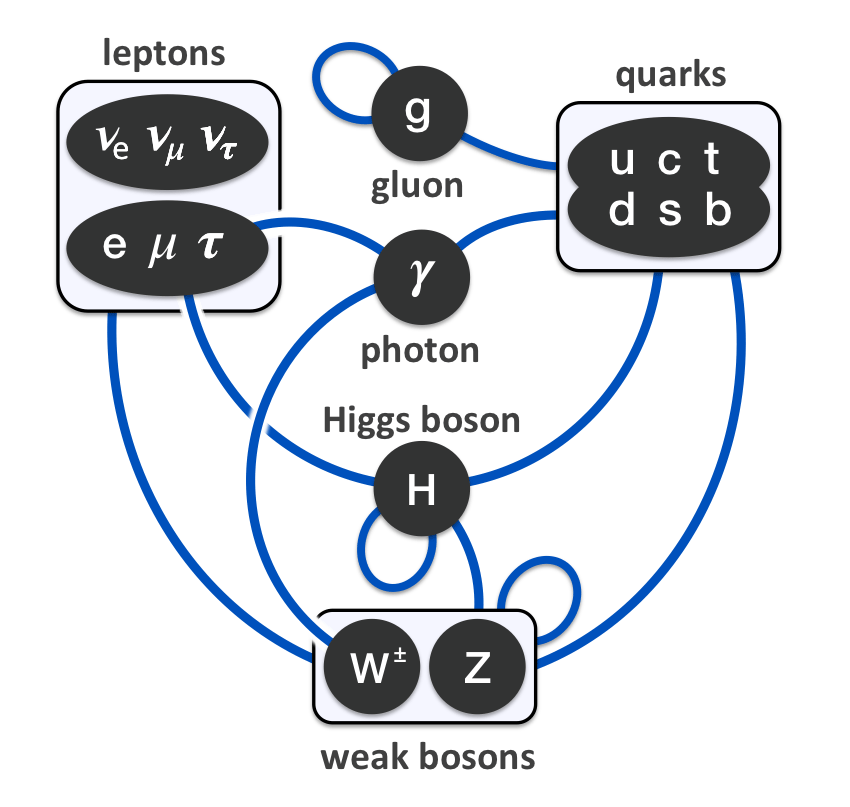
\includegraphics[width=0.55\textwidth]{images/fund_part_in_sm.png}
\label{sm_part_image}
\caption{Illustration of the fundamental particles described by the Standard Model, showing how they interact amongst each other and sometimes themselves. \cite{fund_part_image}}
\end{figure}
\section{Electroweak Unification}
\label{ewk uni}
As previously mentioned the electromagnetic and weak interactions are actually different manifestations of the same electroweak interaction. This is reflected in the \emph{electroweak unification} model; primarily developed by Glashow, Salam, and Weinberg in the 1960s. In 1971 't Hooft and Veltmann showed that the model is renormalisable\footnote{A renormalisable gauge theory is one in which any infinities introduced by the inclusion of higher-order diagrams can be absorbed by modification of a finite number of parameters. All the gauge theories of the Standard Model are renormalisable. In contrast General Relativity isn't renormalisable, leading to problems for theories attempting to include Quantum Gravity.} \cite{renorm1,renorm2,renorm3,renorm4} which has been confirmed by many subsequent particle physics experiments \cite{SM_fit}. The full electroweak theory has a non-abelian symmetry $\mathbf{SU}(2) \otimes \mathbf{U}(1)$; with three gauge bosons $ \left\{ W_{\mu}^{1},W_{\mu}^{2},W_{\mu}^{3} \right\} = \mathbf{W}_{\mu}$ being associated with $\mathbf{SU}(2)$ and one gauge boson $B_{\mu}$ being associated with $\mathbf{U}(1)$. The physical interpretation of the fact that the symmetry is non-abelian is that the $W_{\mu}$ and $B_{\mu}$ bosons interact amongst themselves and with each other.

However the symmetry is broken. The mixing of the wavefunctions for the $W_{\mu}^{3}$ and $B_{\mu}$  results in the neutral Z-boson and the photon; while the remaining $W_{\mu}^{1}$ and $W_{\mu}^{2}$ result in the charged $W^{\pm}$ bosons. The reason why the wavefunctions mix to form the neutral bosons, and why the photons is massless while the W and Z bosons are not, is understood in the context of \emph{spontaneous symmetry breaking} and the Higgs mechanism.
\section{Electroweak Symmetry Breaking}
\label{Higgs_section}
In the SM, the electroweak symmetry is spontaneously broken resulting in masses for the weak bosons and fermions via the Higgs mechanism.

To demonstrate this consider a complex scalar field $\phi$, representing the Higgs field. It is taken to have hypercharge\footnote{Hypercharge $Y$ is a number related to electric charge Q via the Gell-Mann-Nishijima formula: $ Y = 2(Q - T_{3})$, where $T_{3}$ is the third component of weak isospin ($ \pm 1/2$ for left-handed fermion and $0$ for right-handed fermions).} $Y = +1$, weak isospin $1/2$, and transforms as a doublet\footnote{\emph{Multiplet} is a common name for a wavefunction with multiple components. So a doublet has two components, a triplet has three, etc.} under $\mathbf{SU}(2)$.

In analogy with classical mechanics, the Lagrangian is consider in kinetic and potential parts:
\begin{eqnarray}
T &=& \left( D_{\mu} \phi \right) ^{\dagger} D^{\mu} \phi \\
V &=& -\mu^{2} | \phi | ^{2} + \lambda | \phi | ^{4},
\end{eqnarray}
where $D_{\mu}$ is the covariant derivative defined as:
\begin{equation}
D_{\mu} \equiv \partial_{\mu} - ig \frac{\sigma ^{a}}{2} W_{\mu}^{a} - i \frac{g'}{2}B_{\mu},
\end{equation}
$\mu ^{2}$ and $\lambda$ are real constants, $\sigma^{a}$ are the Pauli spin matrices, $g$ is the weak coupling and $g'$ the hypercharge coupling (both dimensionless), and the latin indices run $a = (1,2,3)$.

Assuming $\mu^{2}$ and $\lambda$ are positive implies that the ground state of the system (it's vacuum) will have a non-zero \emph{vacuum expectation value} (VEV). The potential $V$ is solely a function of the magnitude of $\phi$ and takes the form of the (famous) Mexican hat potential (see figure \ref{mexican_hat}). This means that there is no inherent single vacuum (ground state). Defining:
\begin{equation}
v = \sqrt{\mu^{2}/\lambda},
\end{equation}
the VEV can be chosen to be:
\begin{eqnarray}
\left< \phi \right> = \frac{1}{\sqrt{2}}
	\begin{pmatrix}
	0 \\
	v
	\end{pmatrix}.
\end{eqnarray}
The choice of vacuum breaks the electroweak symmetry. It is called \emph{spontaneous} because it occurs without any external interference. Left to its own devices, the system will tend to an inherently asymmetrical vacuum. Note that while the $\mathbf{SU}(2)$ symmetry is broken, the $\mathbf{U}(1)$ symmetry of the electromagnetic interaction remains intact.
\begin{figure}
\centering
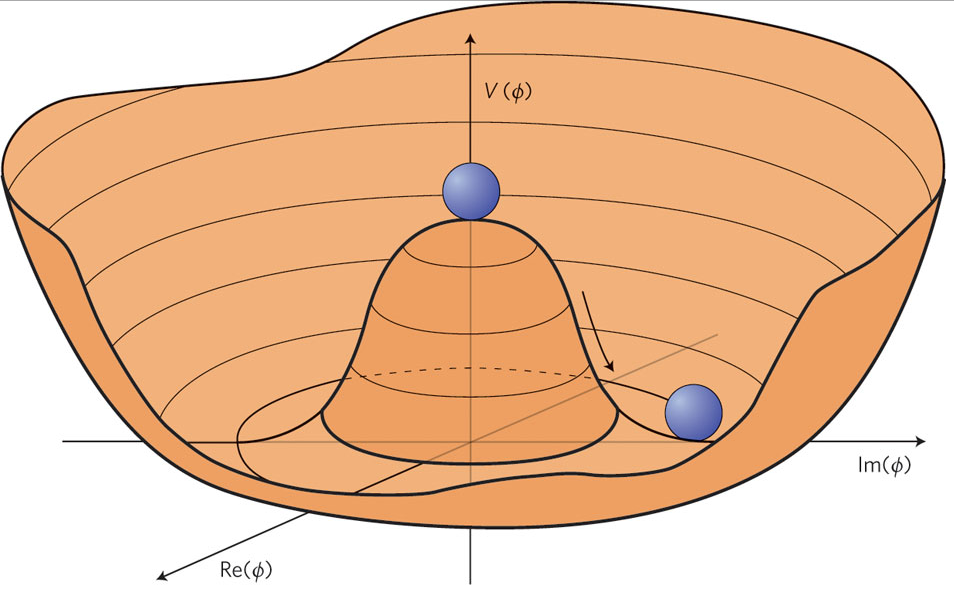
\includegraphics[width=0.65\textwidth]{images/higgs_potential.png}
\caption{Illustration of the Higgs potential. Note that it has a local maximum at the origin and a continuous ring of minima. \cite{mexican_hat}}
\label{mexican_hat}
\end{figure}
This VEV can be inserted into the kinetic term of the Lagrangian. In order to identify the mass terms, compare with the Klein-Gordon Lagrangian:
\begin{equation}
\mathcal{L} = \frac{1}{2} \left( \partial_{\mu} \phi \right) \left( \partial^{\mu} \phi \right) - \frac{1}{2}m^{2}\phi^{2}.
\end{equation}
$m^{2}$ can thus be identified as the coefficient of the quadratic field variable term. The mass terms from the kinetic Lagrangian are then:
\begin{eqnarray}
\Delta T &=& \left< \phi \right> \left( ig \frac{\sigma^{a}}{2}W_{\mu}^{a} + i \frac{g'}{2}B_{\mu} \right) \left(-ig\frac{\sigma^{b}}{2}W_{\mu}^{b} - i\frac{g'}{2}B_{\mu} \right) \left< \phi \right> \\
             &=& \frac{v^{2}}{2}\left( \frac{g^{2}}{4}W_{\mu}^{a}W^{\mu a} + \frac{{g'}^{2}}{4} B_{\mu}B^{\mu} + \frac{gg'}{2} W_{\mu}^{3}B^{\mu} \right).
             \label{mass terms}
\end{eqnarray}
Hence, a mass matrix can be constructed:
\begin{eqnarray}
m^{2} = \frac{v^{2}}{4}
	\begin{pmatrix}
	g^{2} & 0 & 0 & 0 \\
	0 & g^{2} & 0 & 0 \\
	0 & 0 & g^{2} & gg' \\
	0 & 0 & gg' & {g'}^{2}
	\end{pmatrix},
\end{eqnarray}
such that:
\begin{eqnarray}
m^{2} \times
	\begin{pmatrix}
	W_{\mu}^{1} \\
	W_{\mu}^{2} \\
	W_{\mu}^{3} \\
	B_{\mu}
	\end{pmatrix}
\end{eqnarray}
reproduces equation \ref{mass  terms}. The mass matrix can be diagonalised by a suitable choice of basis. Since any basis that diagonalises a matrix is the set of eigenvectors, the corresponding eigenvalues are strung across the (now diagonalised) matrix's diagonal. The canonical choice of eigenvectors and their corresponding eigenvalues are:
\begin{eqnarray}
W_{\mu}^{\pm} = \frac{1}{\sqrt{2}} \left( W_{\mu}^{1} \mp iW_{\mu}^{3} \right), \ m_{W} = \frac{g v}{2} \nonumber \\
Z_{\mu} = \frac{1}{\sqrt{g^{2} + {g'}^{2}}} \left( g'W_{\mu}^{3} - g' B_{\mu} \right), \ m_{Z} = \frac{v}{2}\sqrt{g^{2} + {g'}^{2}} \nonumber \\
A_{\mu} = \frac{1}{\sqrt{g^{2} + {g'}^{2}}} \left( g' W_{\mu}^{3} + g B_{\mu} \right), \ m_{A} = 0.
\end{eqnarray}
The mass eigenvectors are interpreted as the gauge fields for the charged weak, neutral weak, and electromagnetic interactions respectively; with the eigenvalues being the masses of their associated gauge bosons. Due to spontaneously broken $\mathbf{SU}(2)$ theorem symmetry, the W and Z bosons have acquired mass but, as the $\mathbf{U}(1)$ symmetry remains intact, the photon remains massless. This is the \emph{Higgs mechanism}; responsible for giving mass to the W and Z bosons.\footnote{The Higgs mechanism is also responsible for giving mass to fermions, though it is not shown here.}

The \emph{Feynman Calculus} is formulated in terms of deviations from the vacuum. With this in mind one can perturb the Higgs potential by four scalar fields: $w^{1}(x),w^{2}(x),w^{3}(x),$ and $h(x)$. These fields are fluctuations about the vacuum. The perturbed Higgs potential is:
\begin{eqnarray}
\phi =
	\begin{pmatrix}
	w^{1}(x) + iw^{2}(x) \\
	v + h(x) + iw^{3}(x)
	\end{pmatrix}.
\end{eqnarray}
Inserting the perturbed Higgs potential into the potential term of the Lagrangian yields:
\begin{eqnarray}
\Delta V_{perturbation} &=& \frac{-\mu^{2}}{2} \left[ \left( v + h \right)^{2} + w^{a}w^{a} \right] + \frac{\lambda}{4} \left[ \left( v + h \right)^{2} + w^{a}w^{a} \right]^{2} \nonumber \\
&=& \left( \lambda v^{3} - \mu^{2} v \right)h + \frac{1}{2} \left( 3 \lambda v^{2} - \mu^{2} \right)h^{2} + \frac{1}{2} \left( \lambda v^{2} - \mu^{2} \right) w^{a} w^{a} \nonumber \\
&+& \lambda v \left( h^{3} + hw^{a}w^{a} \right) + \frac{\lambda}{4} \left( h^{4} +2h^{2} w^{a} w^{a} \right) \nonumber \\
&=& \frac{1}{2} \left( 2 \lambda v^{2} \right) h^{2} + \lambda v \left( h^{3} + hw^{a}w^{a} \right) + \frac{\lambda}{4} \left( h^{4} + 2 h^{2}w^{a}w^{a} \right).
\end{eqnarray}
Note that the $h$ field has a mass $m_{h} = \sqrt{2 \lambda v^{2}}$ but that the $w^{a}$ fields are all massless. The $w^{a}$ fields are actually \emph{Goldstone Bosons}\footnote{Goldstone's theorem states that any continuous global symmetry that is spontaneously broken must result in one or more massless scalar (spin-0) particles. These are referred to as Goldstone bosons.}. To see how their presence manifests physically, count the total number of degrees of freedom of the system before and after the Higgs mechanism. Prior to the Higgs mechanism, each of the four massless gauge fields has two degrees of freedom (transverse polarisations), for a total of eight, and we have four scalar fields, each with one degree of freedom, for a grand total of 12. After the Higgs mechanism, the Goldstone bosons are ``eaten'' by the now massive gauge fields which subsequently gain an extra degree of freedom (longitudinal polarisation\footnote{For a massless gauge boson, it is always possible to choose a gauge in which the longitudinal polarisation vector is zero. Due to the gauge freedom associated with a massless gauge field, the longitudinal polarisation vector has no physical significance in any gauge. However, in the case of a massive gauge boson, the freedom to choose an arbitrary gauge is lost and the longitudinal polarisation vector does not vanish and now has undeniable physical significance. See \cite{schwartz} for details.}). That's then three degrees of freedoms for each of the three massive gauge fields, plus the two from the massless photon, and one more from the Higgs field for a grand total of 12---matching the system total prior to the Higgs mechanism.
\section{Introduction to Same-Sign W-boson Scattering}
\label{ssWW_intro}
As mentioned in section \ref{ewk uni}, the fact that the electroweak symmetry is non-abelian indicates that the gauge bosons interact amongst themselves. The theory predicts the existence of both \emph{triple gauge couplings} (TGCs) and \emph{quartic gauge couplings} (QGCs) (see figure \ref{tgcs and qgcs}).

\begin{figure}
\centering
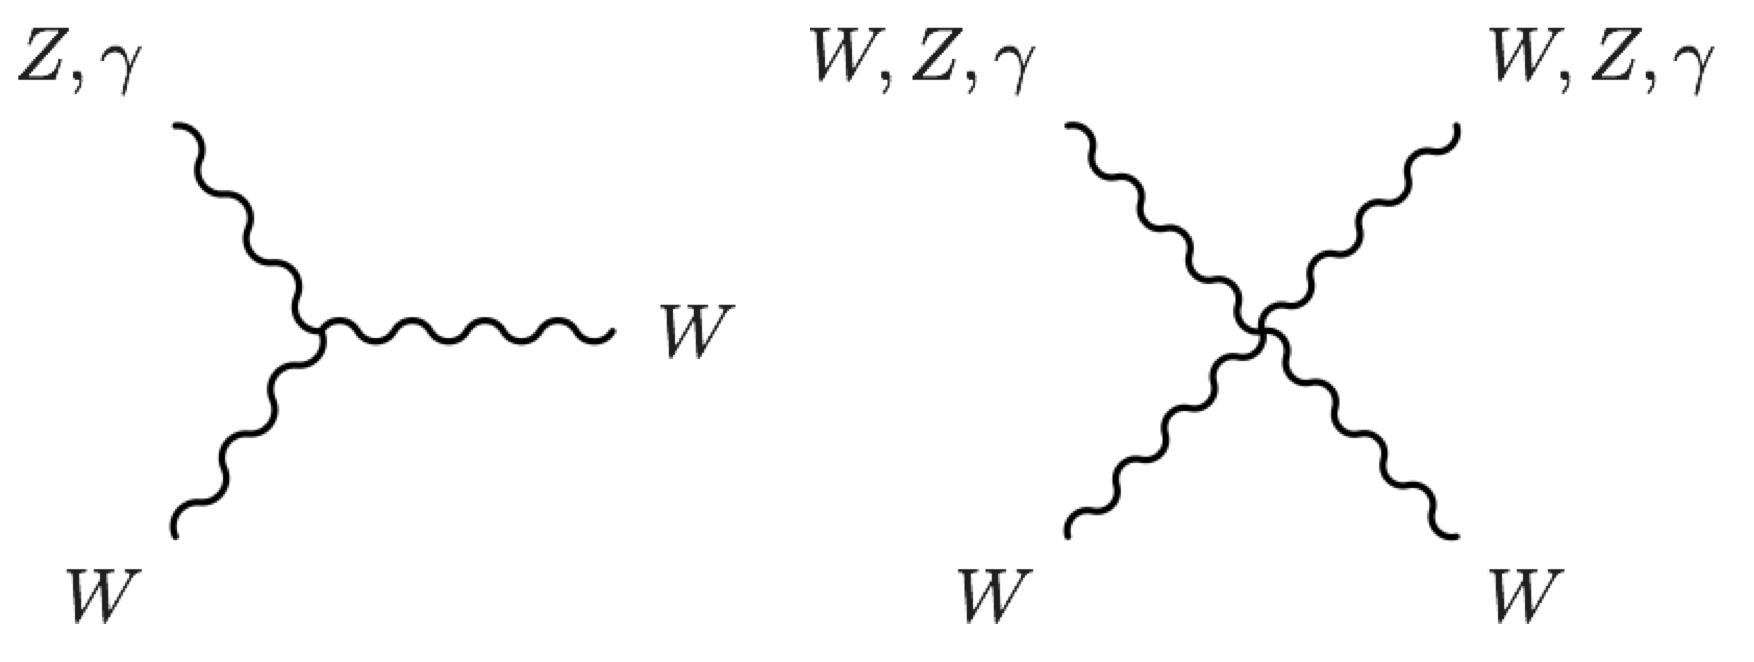
\includegraphics[width=0.65\textwidth]{images/ssWW/vb_self_int.png}
\caption{Feynman diagrams for triple and quartic gauge couplings amongst electroweak gauge bosons. The non-abelian nature of the electroweak force predicts that the gauge bosons can have self-interactions. There are, however, no neutral self-interactions.}
\label{tgcs and qgcs}
\end{figure}

TGCs were extensively studied at the Large Electron-Positron collider \cite{LEP_tgc1,LEP_tgc2,LEP_tgc3,LEP_tgc/qgc2} and the Tevatron \cite{Tevatron_tgc1,Tevatron_tgc2,Tevatron_tgc3} but no evidence was found for QGCs \cite{LEP_tgc/qgc2,LEP_qgc2,LEP_qgc1,Tevatron_qgc2}. The higher energies available at the Large Hadron Collider (LHC) allowed the previously elusive QGCs to be observed \cite{qgc_lhc1,qgc_lhc2,qgc_lhc3}. There are three possible means to investigate QGCs: \textit{tri-boson production}, \textit{exclusive VV production}, and \textit{vector boson scattering} (VBS); see figure \ref{vv_prod}. However tri-boson production has a low cross-section \cite{triboson1,triboson2} and studies of exclusive $VV$ production are complicated by pile-up at hadron colliders \cite{exclusive1,exclusive2}. In contrast VBS has a higher cross-section and distinctive final state VVjj. During the LHC's Run I, the same-sign W-boson scattering cross-section was measured by the ATLAS and CMS collaborations to a significance of 3.6 \cite{ssWW} and 2.0 \cite{ssWW_CMS} standard deviations respectively. More recently, the CMS collaboration published a result using data from the LHC's Run 2, where the cross-section was measured to a significance of 5.5 standard deviations \cite{ssWW_CMS_Run2}.

\begin{figure}
\centering
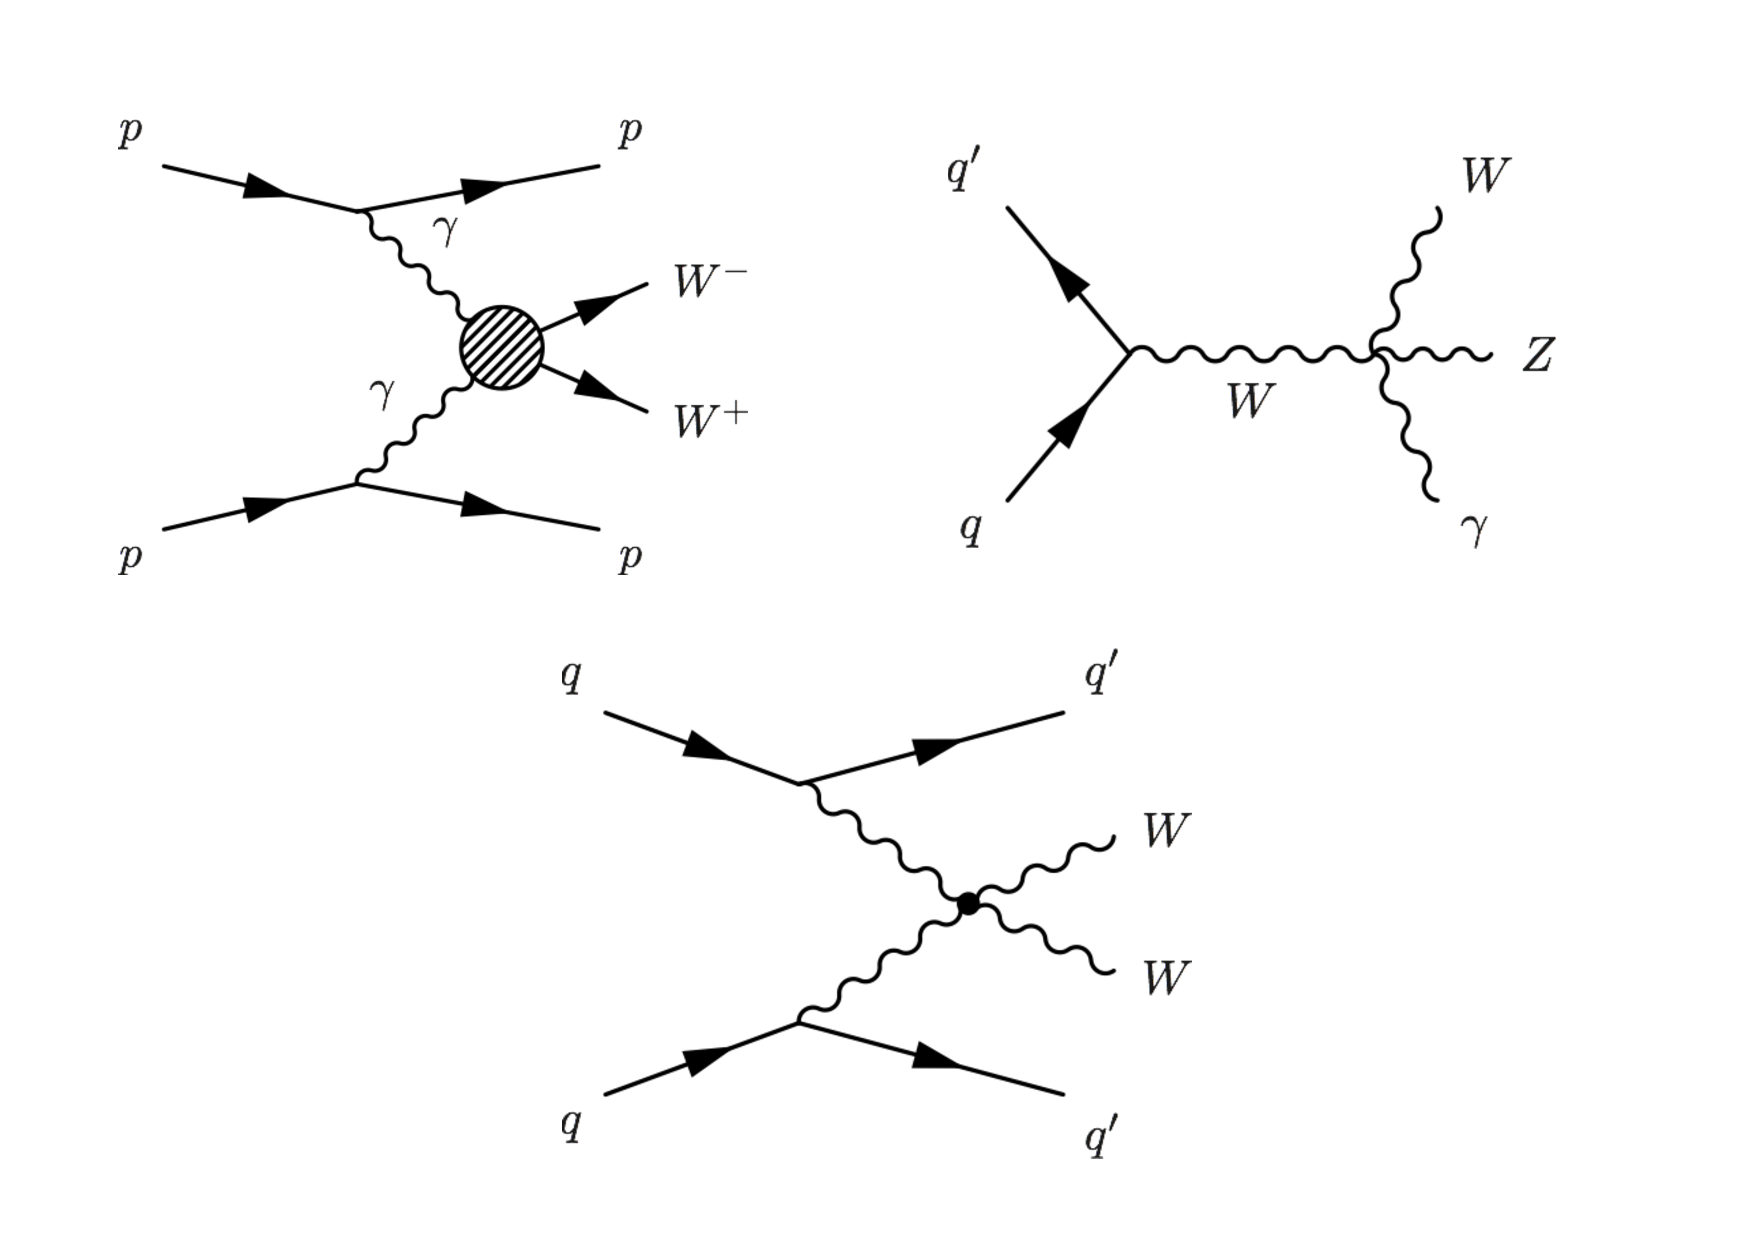
\includegraphics[width=0.85\textwidth]{images/ssWW/VV_prod.pdf}
\caption{Three possible processes for investigating QGCs: at the top on the left, tri-boson production; on the top right, exclusive VV production; and at the bottom, vector boson scattering.}
\label{vv_prod}
\end{figure}

As was discussed in section \ref{Higgs_section}, through the Higgs mechanism, the W and Z-bosons acquire mass which can be interpreted as the longitudinal polarisation component. Without a light SM Higgs-boson, the cross-section for longitudinally polarised VV scattering increases linearly with centre-of-mass energy and violates unitarity at approximately 1 TeV \cite{ssWW} (see figure \ref{x-section_lon_pol_scatt_no_higgs}).

\begin{figure}
\centering
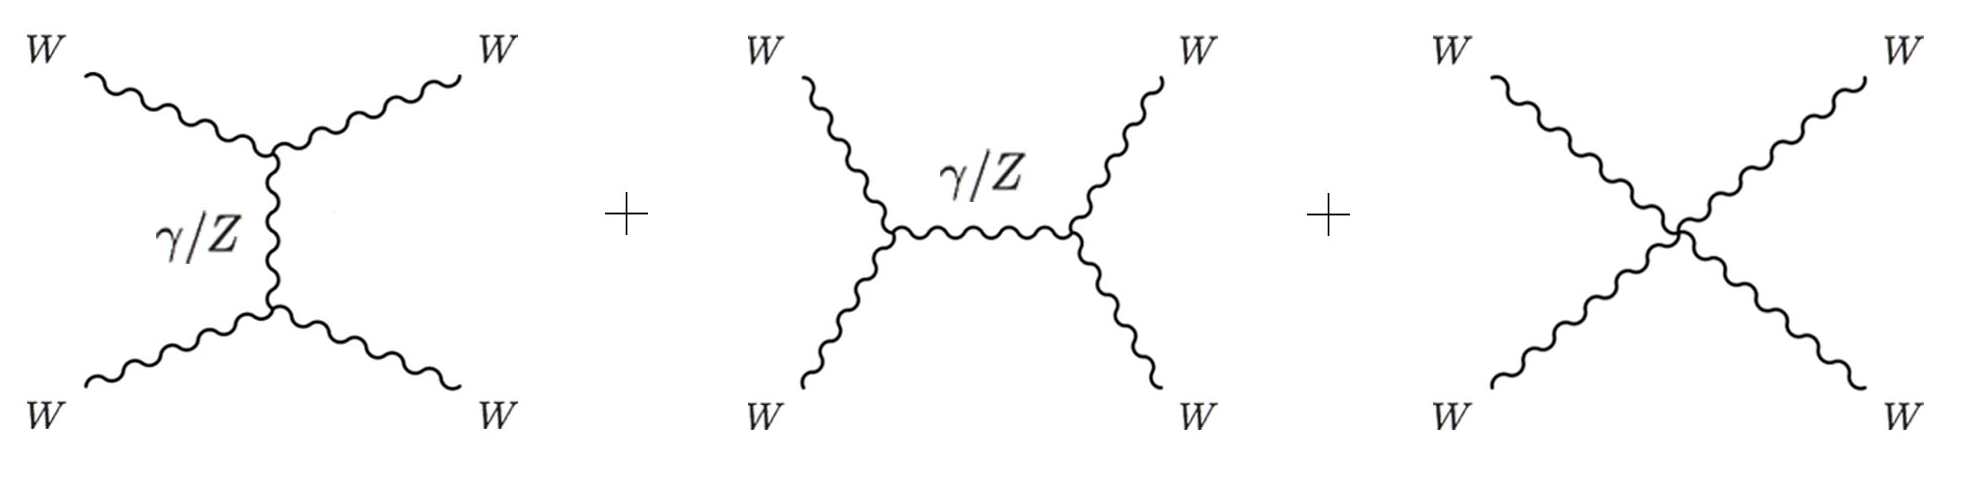
\includegraphics[width=1.\textwidth]{images/ssWW/ww_scatt_diags.png}
\caption{Leading-order Feynman diagrams for $WW \longrightarrow WW$ in the absence of a light SM Higgs-boson.}
\label{ww_scatt_diags}
\end{figure}
\begin{figure}
\centering
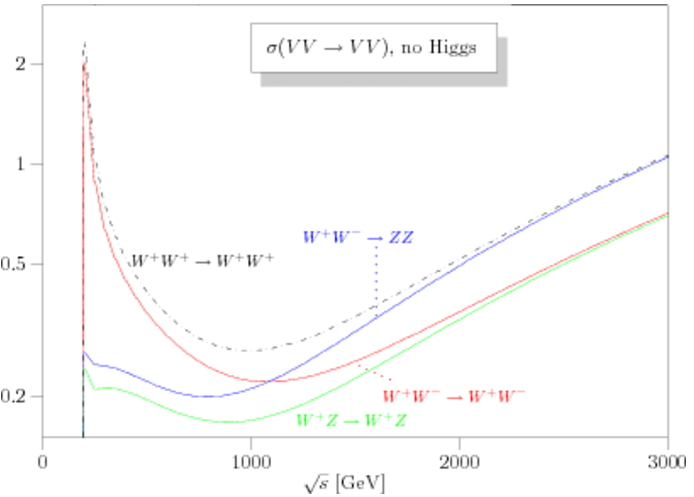
\includegraphics[width=.65\textwidth]{images/ssWW/x-section_lon_pol_scatt_no_higgs.png}
\caption{Longitudinally polarised $VV \longrightarrow VV$ cross-section (in nanobarns) behaviour with $\sqrt{s}$ for four different vector boson scattering processes in the absence of a Higgs-boson. Note that unitarity is violated at approximately 1 TeV. \cite{Alboteanu}}
\label{x-section_lon_pol_scatt_no_higgs}
\end{figure}

However the existence of a light SM Higgs-boson introduces additional diagrams (see figure \ref{new_ww_scatt_diags}), the cross-section becomes regularised \cite{ssWW} (see figure \ref{x-section_lon_pol_scatt_with_higgs}) through the introduction of additional diagrams (compare figures \ref{x-section_lon_pol_scatt_no_higgs} and \ref{x-section_lon_pol_scatt_with_higgs}). This is dealt with in more detail in section \ref{ssWW x-section}.

\begin{figure}
\centering
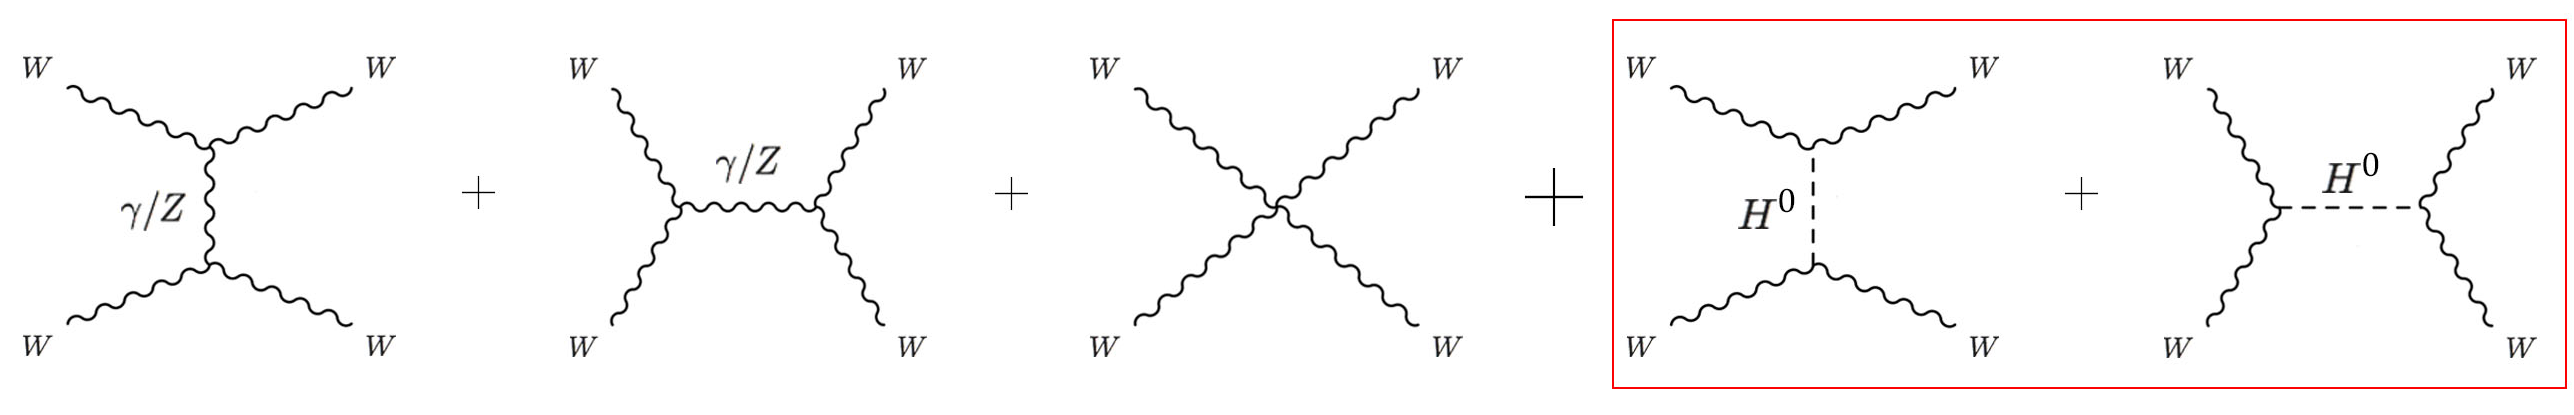
\includegraphics[width=1.\textwidth]{images/ssWW/new_ww_scatt_diags.png}
\caption{Leading-order Feynman diagrams for $WW \longrightarrow WW$ with a light SM Higgs-boson.}
\label{new_ww_scatt_diags}
\end{figure}
\begin{figure}
\centering
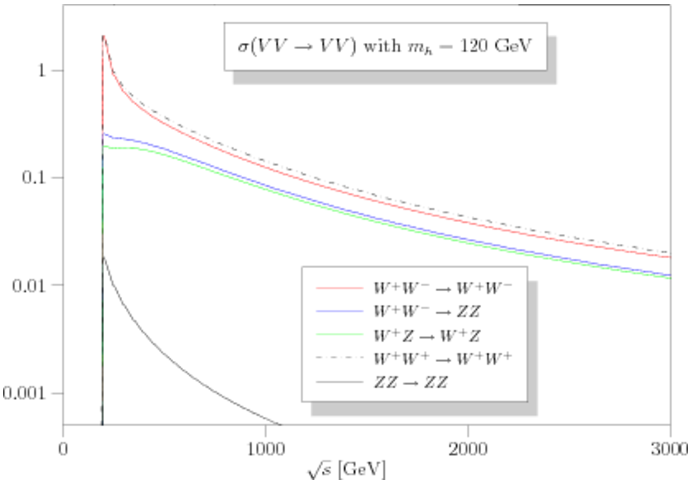
\includegraphics[width=0.65\textwidth]{images/ssWW/x-section_lon_pol_scatt_with_higgs.png}
\caption{Longitudinally polarised $VV \longrightarrow VV$ cross-section behaviour with $\sqrt{s}$ for four different vector boson scattering processes assuming a SM-like Higgs-boson of $120$ GeV mass. The inclusion of the Higgs-boson restores reasonable behaviour of the cross-sections. \cite{Alboteanu}}
\label{x-section_lon_pol_scatt_with_higgs}
\end{figure}

This was a motivation for the existence of a light Higgs-boson prior to its discovery in 2012. At the time of writing this thesis, it is not yet certain whether the 125 GeV Higgs-boson behaves in exactly the way predicted by the SM. VBS could increase understanding of the mechanism of electroweak symmetry breaking. If the vector boson couplings differ from their SM predictions these so-called \emph{anomalous quartic gauge couplings} (aQGCs) may require new physics in order to preserve unitarity, providing additional motivation for studying VBS.

VBS Feynman diagrams are not independently gauge invariant and as a result various non-VBS processes, with the same $VVjj$ final state, must be included in the analysis. These additional non-VBS contributions are classified into electroweak non-VBS production (see figure \ref{ewk_bkg}) and QCD production (see \ref{qcd_bkg}). Certain processes of the non-VBS electroweak production such as VVV or VH production can be gauge invariantly separated and can be suppressed by kinematic cuts. Processes in the QCD production category can be suppressed using topological cuts \cite{ssWW}.

\begin{figure}
\centering
  \centering
  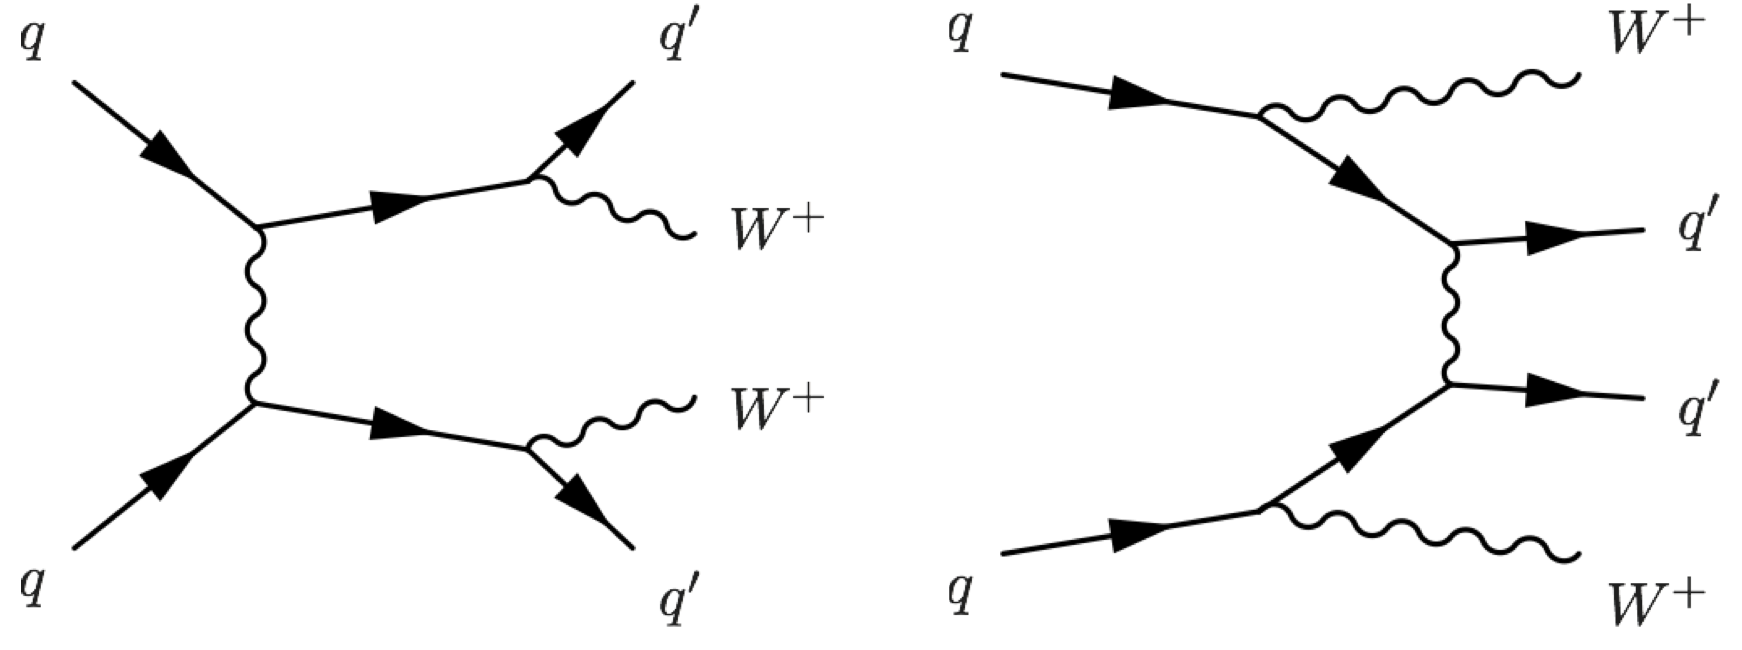
\includegraphics[width=.75\textwidth]{images/ssWW/ewk_bkg.png}
  \caption{Examples of non-VBS electroweak processes with WWjj final state.}
  \label{ewk_bkg}
\end{figure}
\begin{figure}
  \centering
  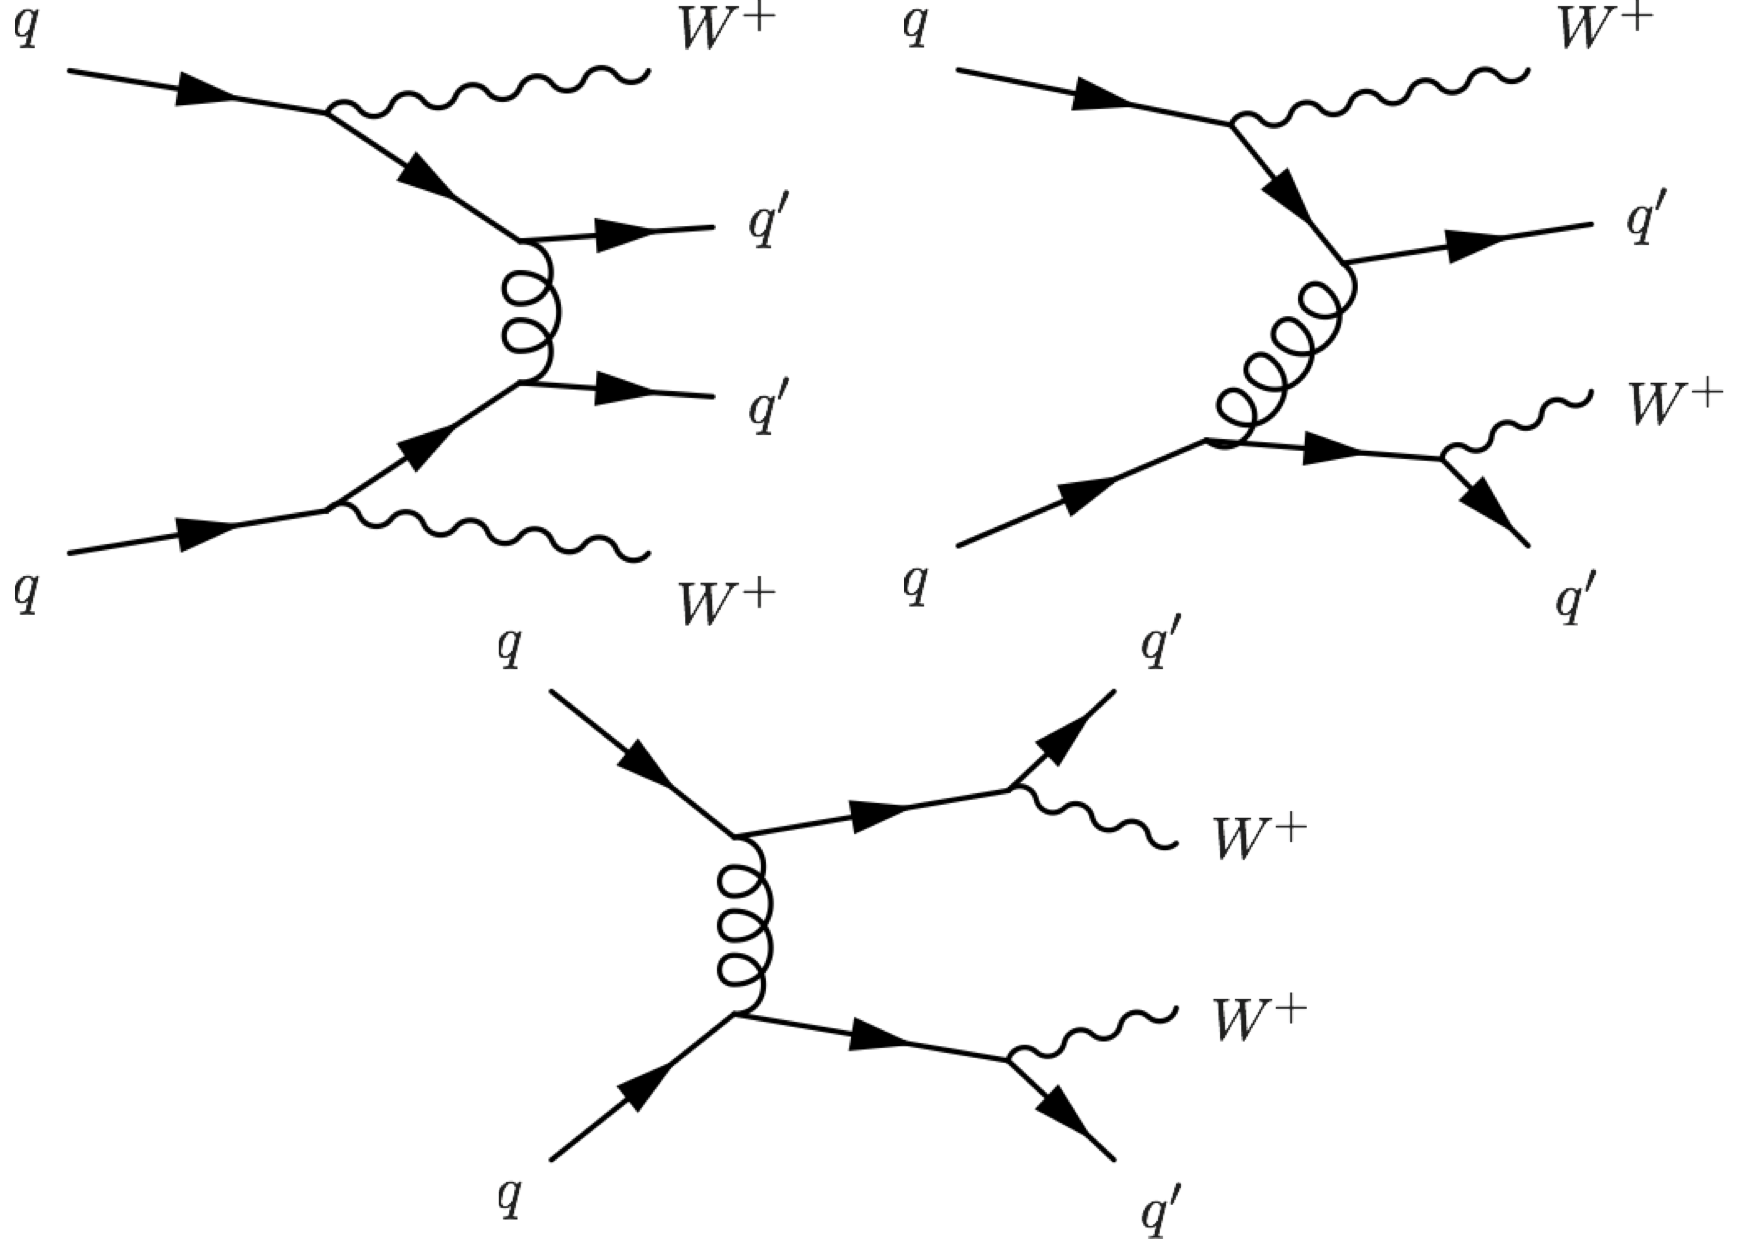
\includegraphics[width=.75\textwidth]{images/ssWW/qcd_bkg.png}
  \caption{Examples of QCD processes with $WWjj$ final state. Can be suppressed by topological cuts.}
  \label{qcd_bkg}
\end{figure}

Vector boson scattering can occur in either the same-sign $W^{\pm}W^{\pm}$ or opposite-sign $W^{\pm}W^{\mp}$ cases. However, the same-sign is preferable for study due to the fact that there is no leading-order gluon-gluon initial state in the same-sign case, in contrast to the opposite-sign case where it does occur (see figure \ref{LO_gluon-gluon}). As a result the $W^{\pm}W^{\pm}jj$ QCD contributions are small when compared to the opposite-sign case (see table \ref{ss_vs_os}). Same-sign W-boson scattering is studied experimentally in the di-lepton channels, considering only electrons ($e$'s) and muons ($\mu$'s), i.e. in the channels $e^{\pm}e^{\pm},e^{\pm}\mu^{\pm},\mu^{\pm}\mu^{\pm}$.\footnote{$\uptau$-leptons are not considered as they are experimentally harder to detect.}

\begin{figure}
\centering
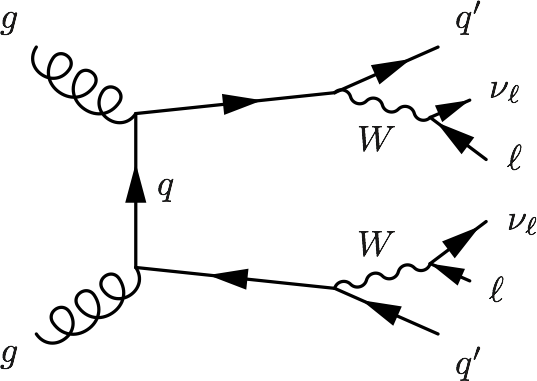
\includegraphics[width=0.4\textwidth]{images/ssWW/LO_gluon-gluon.png}
\caption{Leading-order gluon-gluon $WW$ production. Only possible in the opposite-sign case.}
\label{LO_gluon-gluon}
\end{figure}

\begin{table}
\centering
\begin{tabular}{c c c c}
\hline \hline
Final State & Process & $VVjj$-EW & $VVjj$-QCD \\ \hline 
$\ell^{\pm}\nu\ell^{'\pm}\nu^{'}jj$ (same sign, arbitrary flavour) & $W^{\pm}W^{\pm}$ & $19.5$ fb  & $18.8$ fb \\
$\ell^{\pm}\nu\ell^{'\mp}\nu^{'}jj$ (opposite sign, arbitrary flavour) & $W^{\pm}W^{\mp}$ & $91.3$ fb & $3030$ fb \\
\hline \hline
\end{tabular}
\caption{Comparison of the cross-sections for electroweak and QCD production for both the same-sign and opposite-sign final states at $\sqrt{s}=13$. Note that for the same-sign case the electroweak and QCD cross-sections are the same order of magnitude while this is not true for the opposite sign case. \cite{ssWW}}
\label{ss_vs_os}
\end{table}

Thus same-sign W-boson scattering represents the most promising approach to observe VBS, since the electroweak and QCD contributions are of the same order of magnitude. The distinctive experimental signature is two same-sign leptons, two forward jets, and $E_{T}^{miss}$ carried away by the neutrinos (see figure \ref{ssWW_topology}). Selecting specifically for forward jets helps suppress the QCD background from processes such as quark-quark, or gluon-gluon scattering plus VV radiation, or electroweak VV production plus radiation of gluons resulting in jets. The tagging jets are defined to be the two jets with the highest $p_{T}$ in an event. The tagged jets in $W^{\pm}W^{\pm}jj$ electroweak events tend have a greater difference in rapidity and invariant mass than those in $W^{\pm}W^{\pm}jj$ QCD events. They also tend tend have a larger individual rapidities than their QCD counterparts.

\begin{figure}
\centering
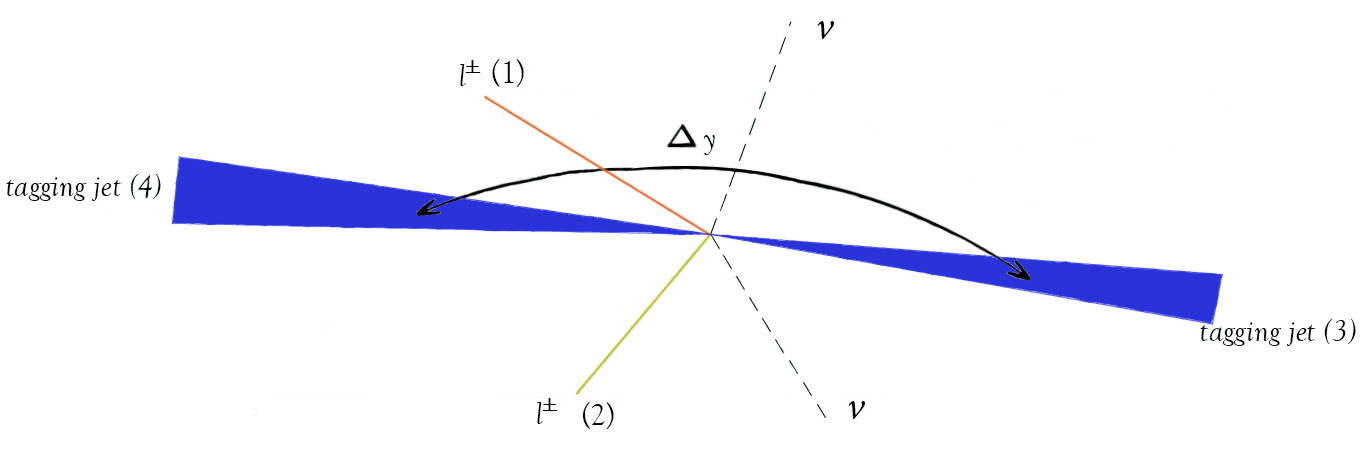
\includegraphics[width=1.0\textwidth]{images/ssWW/ssWW_topology.jpg}
\caption{An illustration of the VBS event topology. Note the charged leptons from the W decay (1,2) and the forward tagging jets (3,4). The invisible neutrinos escape, detectable only through their missing transverse energy. Modified from an image in \cite{ssWW_int_note}.}
\label{ssWW_topology}
\end{figure}

\section{$W^{\pm}W^{\pm}$ Scattering Cross-Section}
\label{ssWW x-section}
Defined initially, in the context of $2\longrightarrow 2$ scattering, are the Lorentz invariant Mandelstam variables:
\begin{eqnarray}
s &=& \left( p - k \right)^{2} = \left( p' + k' \right)^{2} \nonumber \\
t &=& \left(p' - p \right)^{2} = \left(k' - k \right)^{2} \nonumber \\
u &=& \left(k' - p \right)^{2} = \left( p' - k \right)^{2},
\end{eqnarray}
where $p$ and $k$ are the momenta of the initial state particles, and $p'$ and $k'$ are the momenta of the final state particles.

The fact that the electroweak interaction has a non-abelian gauge symmetry means that the gauge bosons are free to scatter off each other. The leading order diagrams for $W^{\pm}W^{\pm}$ scattering that do not involve a Higgs-boson shown in figure \ref{diagrams no higgs}
\begin{figure}
\centering
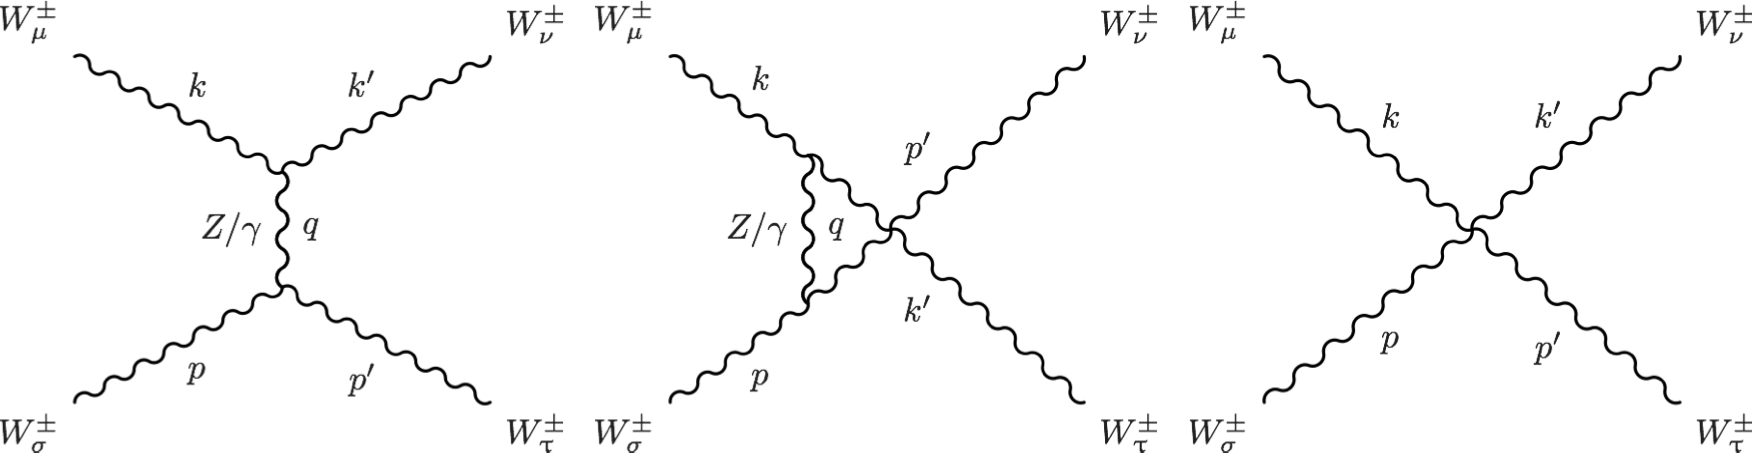
\includegraphics[width=1.0\textwidth]{images/ssWW/diagrams_no_higgs.png}
\caption{Leading-order Feynman diagrams for same-sign W-boson scattering that do not involve a Higgs-boson. Note that the $t$ (left) and $u$ (middle) channel diagrams involve TGCs while the remaining (right) one involves a QGC.}
\label{diagrams no higgs}
\end{figure}

In order to see how the longitudinally polarised scattering amplitude violates unitarity at high energies, apply the Feynman rules for electroweak theory\footnote{See, for example, \cite{mann} or \cite{griffiths}.} to the leading order Feynman diagrams. For the $t$-channel diagram:
\begin{eqnarray}
i \mathcal{M} =& i \hat{\epsilon}_{\mu}(k)\hat{\epsilon}_{\nu}^{*}(k') \left[G^{\mu \nu} \left( k - k' \right)^{\rho} - g^{\mu \rho} \left(q + k \right)^{\nu} + g^{\rho \nu} \left( q + k' \right)^{\mu} \right] \nonumber \\
& \times  \left( \frac{g^{2}c_{W}^{2}}{q^{2} - m_{Z}^{2}} + \frac{g^{2}s_{W}^{2}}{q^{2}} \right)g_{\lambda \rho} \nonumber \\
& \times \left[ g^{\sigma \uptau} \left(p - p' \right)^{\lambda} - g^{\sigma \lambda} \left( q + p \right)^{\uptau} + g^{\lambda \uptau}\left(q +k' \right)^{\sigma} \right] \hat{\epsilon}_{\sigma}(p) \hat{\epsilon}_{\uptau}^{*}(p'),
\end{eqnarray}
for the $u$-channel diagram:
\begin{eqnarray}
i \mathcal{M} = & i \hat{\epsilon}_{\mu}(k) \hat{\epsilon}_{\nu}^{*}(p') \left[ g^{\mu \nu} \left( k - p' \right)^{\rho} - g^{\mu \rho} \left(q + k \right)^{\nu} + g^{\rho \nu} \left( q + p' \right) \right] \nonumber \\
& \times \left( \frac{g^{2}c_{W}^{2}}{q^{2}-m_{Z}^{2}} + \frac{g^{2}s_{W}^{2}}{q^{2}} \right)g_{\lambda \rho} \nonumber \\
&\times \left[ g^{\sigma \uptau} \left(p - k' \right)^{\lambda} - g^{\sigma \lambda} \left( q + p \right)^{\uptau} + g^{\lambda \uptau} \left( q + k' \right)^{\sigma} \right] \hat{\epsilon}_{\sigma}(p)\hat{\epsilon}_{\uptau}^{*}(k'),
\end{eqnarray}
and for the QGC diagram:
\begin{eqnarray}
i \mathcal{M} &= i g^{2} \hat{\epsilon}(k) \hat{\epsilon}_{\nu}^{*}(k')\hat{\epsilon}_{\sigma}(p)\hat{\epsilon}_{\uptau}^{*} \left( 2g^{\mu \nu}g^{\sigma \uptau} - g^{\mu \sigma}g^{\nu \uptau} - g^{\mu \uptau}g^{\nu \sigma} \right),
\end{eqnarray}
where $\hat{\epsilon}$ are the polarisation vectors of the W-bosons, $p$ and $k$ are their momenta, $c_{W}$ and $s_{W}$ are the cosine and sine of the weak mixing angle, which is defined in terms of the weak and hypercharge couplings:
\begin{equation}
s_{W} = \frac{g'}{\sqrt{g^{2} + {g'}^{2}}}.
\end{equation}
The W-bosons considered here are longitudinally polarised. If their four-momentum is given by $k_{\mu} = \left( E_{k},0,0,k \right)$, then the longitudinal polarisation vector is $\hat{\epsilon}_{\mu} = \left( \frac{k}{m},0,0,\frac{E_{k}}{m} \right)$. In the high momentum limit $k >> m$, the polarisation vector can be approximated as:
\begin{eqnarray}
\hat{\epsilon}_{\mu} &=& \left( \frac{k}{m},0,0,\frac{E_{k}}{m} \right) \nonumber \\
&=& \frac{1}{m} \left( E_{k} \sqrt{1-\frac{m^{2}}{E_{k}^{2}}},0,0,k\sqrt{1+\frac{m^{2}}{k^{2}}} \right) \nonumber \\
&\approx& \frac{k^{\mu}}{m}.
\end{eqnarray}
By inserting this approximation in the scattering amplitude, it can be seen that there are terms of $\mathcal{O} \left( \frac{s}{m_{W}^{2}} \right)$ and terms of $\mathcal{O} \left( \frac{s^{2}}{m_{W}^{4}} \right)$. Upon summing the amplitudes, however, the latter terms cancel, leaving $\mathcal{M} \propto \frac{s}{m_{W}^{2}}$.

The cross-section for a $2 \longrightarrow 2$ scattering process with particles of equal mass is given by:
\begin{equation}
\sigma = \frac{1}{32 \pi^{2}s} \int \sqrt{1-\frac{4m^{2}}{s}} \abs{\mathcal{M}}^{2} d\Omega
\end{equation} \cite{griffiths}.
Hence $\sigma \propto \frac{s}{m_{W}^{4}}$, which means the cross-section grows indefinitely with energy and will eventually violate unitarity\footnote{Meaning the probability for the scattering to occur will be greater than 1 (unity), which is unphysical.}. This occurs at approximately 1 TeV.

However if a light Higgs-boson is included then additional diagrams are introduced (see figure \ref{diagrams higgs}). The scattering amplitude for the $t$-channel diagram is:
\begin{equation}
i \mathcal{M} = -ig^{2}m_{W}^{2}\frac{\hat{\epsilon}_{\mu}(k)\hat{\epsilon}_{\nu}^{*}(k')g^{\mu \nu}g^{\sigma \uptau}\hat{\epsilon}_{\sigma}(p)\hat{\epsilon}_{\uptau}^{*}(p')}{q^{2}-m_{h}^{2}},
\end{equation}
and for the $u$-channel:
\begin{equation}
i\mathcal{M} = -ig^{2}m_{W}^{2}\frac{\hat{\epsilon}_{\mu}(k)\hat{\epsilon}_{\nu}^{*}(p')g^{\mu \nu}g^{\sigma \uptau}\hat{\epsilon}_{\sigma}(p)\hat{\epsilon}_{\uptau}^{*}(k')}{q^{2}-m_{h}^{2}}.
\end{equation}
Taking the same limit as before, there are again terms of $\mathcal{O}\left( \frac{s}{m_{W}^{2}} \right)$ but of the opposite sign. These opposite sign contributions cancel exactly with the terms from the previous diagrams such that, in the high energy limit, $\mathcal{M} \propto constant$ instead. The cross-section now decreases with energy and is hence regularised.
\begin{figure}
\centering
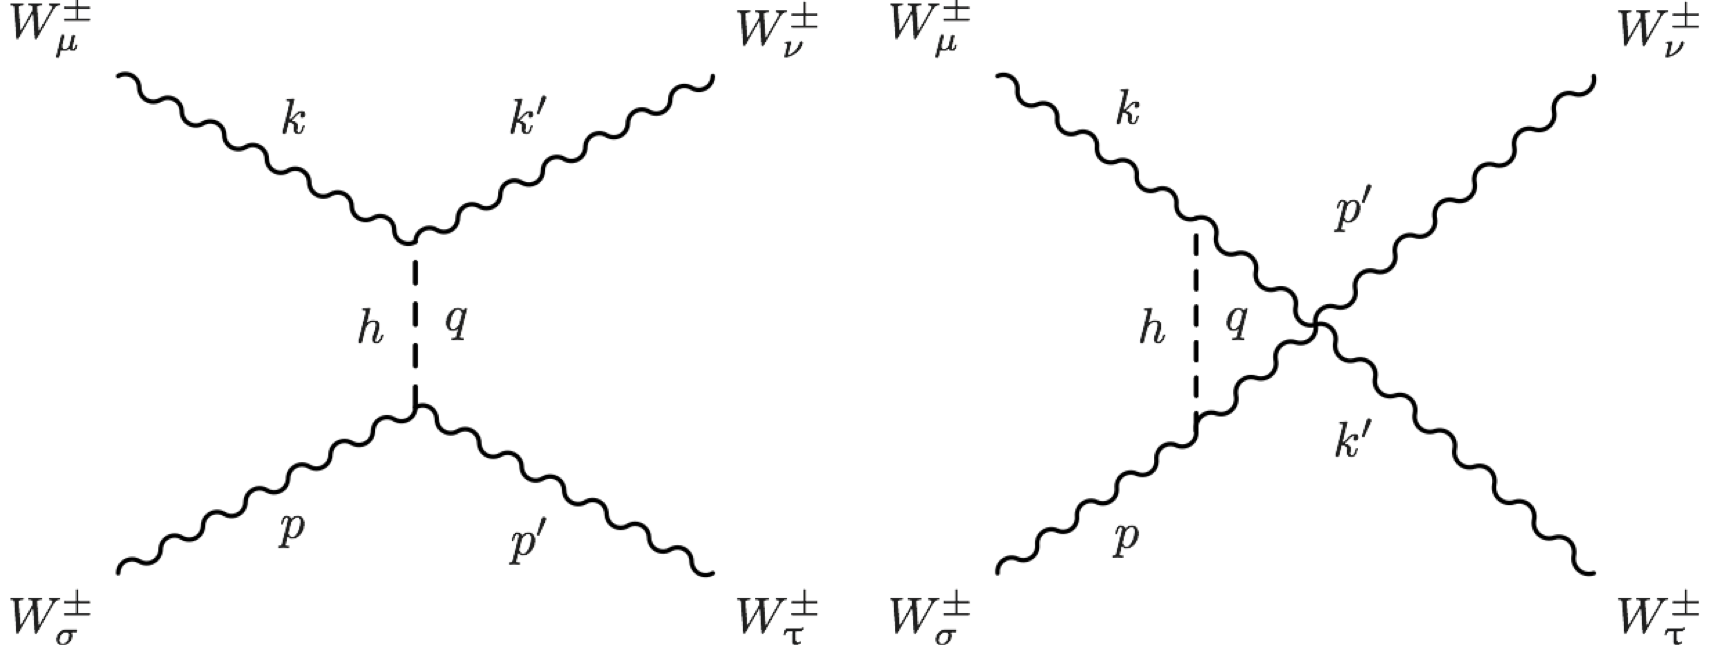
\includegraphics[width=0.75\textwidth]{images/ssWW/diagrams_higgs.png}
\caption{Leading-order Feynman diagrams for same-sign W-boson scattering that involve a Higgs-boson. The $t$-channel diagram is on the left while the $u$-channel diagram is on the right}
\label{diagrams higgs}
\end{figure}
\chapter{The Large Hadron Collider}
The primary reference for this chapter was \cite{LHC} and it should be consulted for further reading.

Constructed by the European Centre for Nuclear Research (CERN), the Large Hadron Collider (LHC) \cite{LHC} is the world's largest particle accelerator. It has provided some of the experimental confirmation of the Standard Model. Located underground and crossing the Franco-Swiss border at four points (most of the tunnel is located in France), the LHC was installed in the existing 26.7 km tunnel that was previously used by the Large Electron-Positron Collider (LEP). Initially approved by the CERN Council in 1994, construction of the LHC received substantial contributions from CERN member-states and non-member states alike. CERN was chosen as the location due to the advantage of being able to use the pre-existing LEP tunnel. Because the LHC is a particle-particle collider (as opposed to a particle-antiparticle collider), it is composed of two rings with counter-rotating beams.\footnote{Particle-antiparticle colliders can have both beams within the same ring \cite{LHC}.} Each of the two beam pipes is kept at ultrahigh vacuum $10^{-10}$ Torr \cite{vacuum} in order to reduce the possibility of undesirable collisions with gas molecules.

The construction of the LHC was primarily approved in order to discover beyond the Standard Model physics. It has two high luminousity\footnote{Both originally aiming for a peak luminousity of $\mathcal{L} = 10^{34}$cm$^{-2}$s$^{-1}$.} experiments: ATLAS (A Toroidal LHC ApparatuS) \cite{ATLAS} and CMS (Compact Muon Solenoid) \cite{CMS}, as well as two low luminousity experiments: LHCb (Large Hadron Collider bottom)\footnote{Originally aiming for a peak luminousity of $\mathcal{L} = 10^{32}$cm$^{-2}$s$^{-1}$.} \cite{LHCb} which is primarily concerned with the physics of b-quarks, and TOTEM (TOTal Elastic and diffractive cross section Measurement)\footnote{Originally aiming for a peak luminousity of $\mathcal{L} = 2 \times 10^{29}$cm$^{-2}$s$^{-1}$.} \cite{TOTEM} which specialises in the detection of small-angle elastic proton scattering.  The LHC is versatile and can also be operated to collide heavy-ions instead of protons. ALICE (A Large Ion Collider Experiment)\footnote{Originally aiming for a peak luminousity of $\mathcal{L} = 10^{27}$cm$^{-2}$s$^{-1}$.} \cite{ALICE} is dedicated to the detection and analysis of these heavy-ion collisions.

As with all particle accelerators, the protons are steered by means of powerful magnetic fields. Colliding the counter-rotating beams of protons requires opposite magnetic fields in both of the LHC rings. However, there is not enough physical space for two separate rings of magnets in the LHC tunnel. In order to compensate for this, the LHC uses twin bore magnets that consist of two sets of coils and beam channels within the same mechanical structure and cryostat. The magnetic system itself consists of 1232 dipole magnets, each with a length of 15 metres, which are concerned with bending the proton beams, and 392 quadrupole magnets of lengths varying between five and seven metres which are concerned with focusing the beam. This magnet system produces fields above 8 T and is kept at a temperature of 2 K by approximately 96 tonnes of superfluid helium-4, making the LHC the world's largest cryogenic facility \cite{cryo}.

The LHC is fed with protons by means of the injector chain: a series of accelerators that successively increase the energy of the protons. The accelerators that make up the injector chain were previously existing accelerators at CERN which were repurposed and upgraded in order to provide the LHC with protons. In order of increasing energy the constituents of the injector chain are: \emph{Linac2}, \emph{Proton Synchrotron Booster} (PSB), \emph{Proton Synchrotron} (PS), and ultimately the \emph{Super Proton Synchrotron} (SPS) which then supplies protons for use by the LHC. The injector chain is illustrated in figure \ref{lhc_injectors_image}.

\begin{figure}
\centering
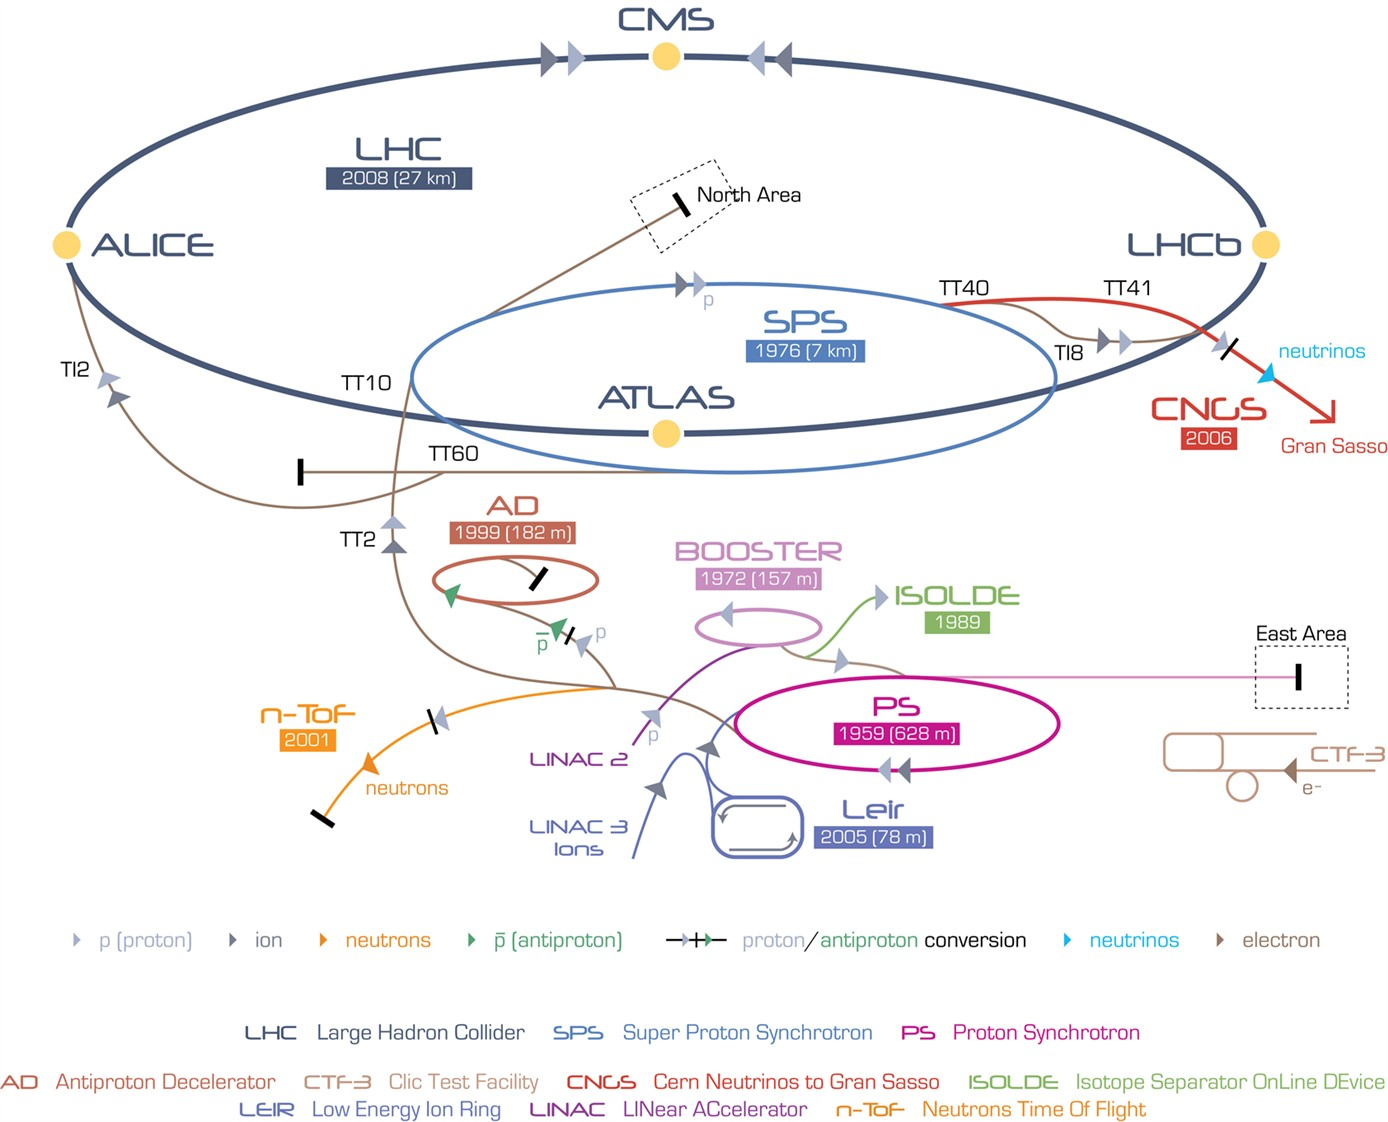
\includegraphics[width=.93\textwidth]{images/lhc_injectors.png}
\caption{Illustration of the LHC's injector chain. \cite{lhc_injector_image}}
\label{lhc_injectors_image}
\end{figure}
\chapter{The ATLAS Detector}
The primary reference for this chapter was \cite{ATLAS} and it should be consulted for further reading.
\section{Overview}
\label{atlas_overview}
The ATLAS (A Toroidal LHC Apparatus) detector \cite{ATLAS} is one of two general purpose detectors at the LHC (the other being the CMS detector). It is capable of probing both proton-proton and heavy-ion collisions.

In the coordinate system used for the ATLAS detector, the nominal interaction point is defined to be the origin; while the z-axis is defined along the beam-line, and the x-y plane transverse to the beam-line. The positive x-direction points centripetally (towards the centre of the LHC ring) and the positive y-direction is defined as pointing upwards. The azimuthal angle $\phi$ is measured around the beam axis while the polar $\theta$ angle is measured from the beam axis. Commonly used in place of the polar angle $\theta$ is pseudorapidity $\eta$, which is defined as $\eta = -\ln \tan(\theta /2)$. In cases where an object had a non-negligible mass, such as a jet, rapidity is preferred and is defined as $y = \frac{1}{2} \ln \left( \frac{E+p_{z}}{E-p_{z}} \right) $. Rapidity and pseudorapidity are favoured because (unlike the polar angle) differences in these quantities are Lorentz invariant. The azimuthal angle along with pseudorapidity is used to define a useful spacial quantity $\Delta R$, defined as $\Delta R = \sqrt{\Delta \eta ^{2} + \Delta \phi ^{2}}$. It is useful to define certain kinematic quantities in the transverse x-y plane such as transverse momentum $p_{T}$, transverse energy $E_{T}$, and missing transverse energy $E_{T}^{miss}$.

\begin{figure}
\centering
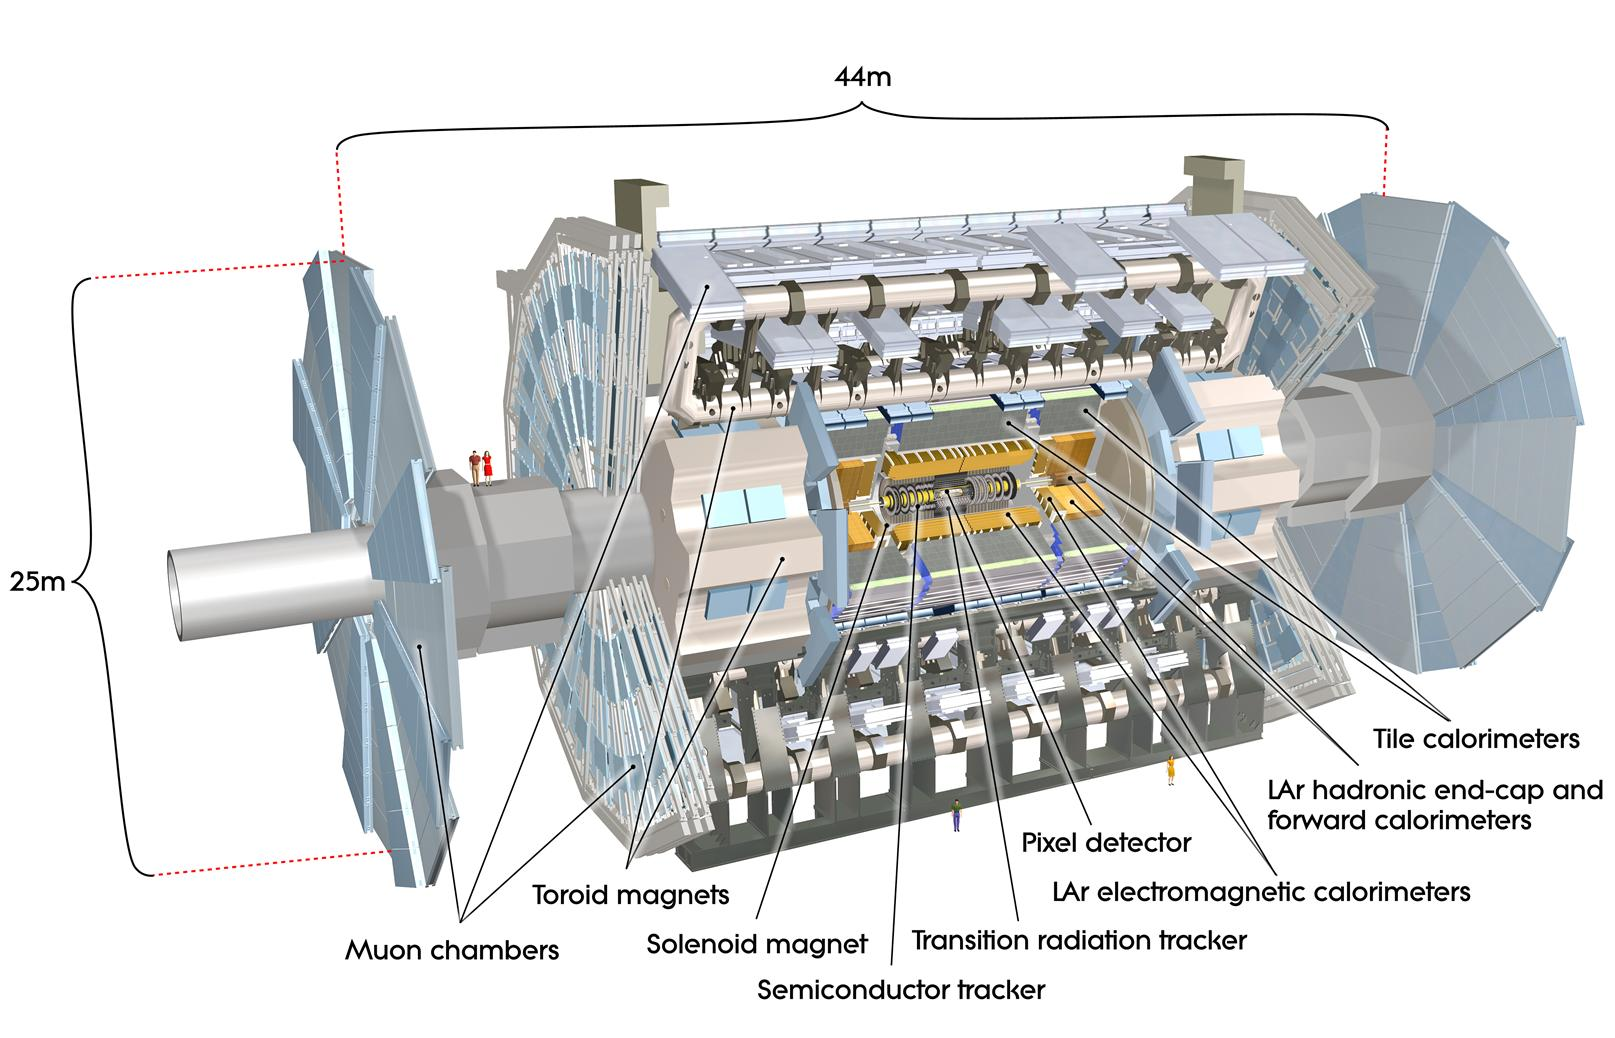
\includegraphics[scale=0.25]{images/image_AtlasDetector.png}
\caption{A cut-away view of the ATLAS detector with its dimensions and some selected components labelled. \cite{ATLAS}}
\label{AtlasDetector}
\end{figure}

The ATLAS detector itself is approximately 25 metres high, approximately 44 metres long, and weighs about 7000 tonnes. Its azimuthally symmetric design means that it is forward-backward symmetric about the interaction point (see figure \ref{AtlasDetector}). The detector's own system of magnets consist of a superconducting solenoid which surrounds the inner-detector; as well as three superconducting toroids: the barrel toroid and the two end-cap toroids. The superconducting solenoid (see figure \ref{magnet_sol}) runs parrallel with the beam-pipe and is designed to produce an axial 2 T magnetic field for the inner detector. The barrel toroid along with the two end-cap toroids (see figure \ref{magnets_tor}) serve to produce to a toroidal magnetic fields of 0.5 T and 1 T for use of the muon detectors in the barrel and end-cap regions respectively. The ATLAS detector has a 38 metre long beam-pipe section with a central chamber surrounding the interaction point. The central chamber houses the pixel detector, which forms the innermost component of the inner-detector (the other components being the SCT and TRT detectors). The inner-detector is capable of measuring the momentum of charged particles and identifying the interaction vertices, among other things. Surrounding the inner-detector is the Liquid Argon (LAr) electromagnetic calorimeter. This is a sampling calorimeter with a coverage of $|\eta | < 3.2$. This, in turn, is surrounded by the scintillating tile hadronic calorimeter (also sampling) which covers the range $ |\eta| < 1.7$. These descriptions apply to the calorimetry systems in the barrel. Supplementing the calorimetry systems in the barrel are the LAr forwards calorimeters. These extend the effect range of the calorimetry system to $ | \eta| = 4.9$ for both electromagnetic and hadronic energy measurements. The calorimetry system is surrounded by the muon spectrometer which defines the overall dimensions of the ATLAS detector.

\begin{figure}
\centering
\begin{minipage}{0.5\textwidth}
  \centering
  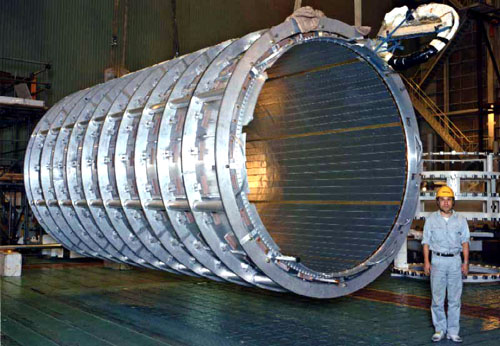
\includegraphics[width=0.7\linewidth]{images/image_solenoid_magnets.jpg}
  \captionof{figure}{The superconducting solenoid after completion of the coil winding, prior to installation. \cite{ATLAS}}
  \label{magnet_sol}
\end{minipage}%
\begin{minipage}{0.5\textwidth}
  \centering
  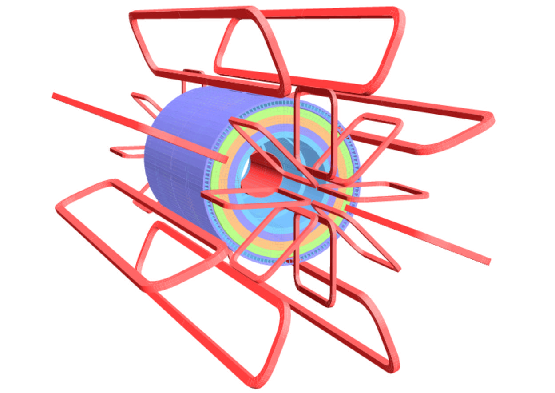
\includegraphics[width=1.0\linewidth]{images/image_toroid_magnets.png}
  \captionof{figure}{Geometry of the eight barrel toroid coils and the end-cap toroid coils. \cite{ATLAS}}
  \label{magnets_tor}
\end{minipage}
\end{figure}

The ATLAS trigger system for Run 2 is divided into two parts: the hardware-based first level trigger (L1-Trigger) \cite{l1_trigger} and the software-based high-level trigger (HLT) \cite{hlt}.

Since the design luminousity of the LHC means that high levels of radiation are present at the interaction point, the ATLAS detector needs to rely on approximately 300 tonnes of shielding in order to reduce both backgrounds and to protect the detector components and electronics from radiation damage and ageing \cite{ATLAS}. The shielding is structured in three layers, with the inner layer intended to stop high energy hadrons and secondary interactions, the second layer designed to moderate neutron radiation escaping from the first layer, and the third layer used to stop photon radiation (a by-product of the neutron capture process of the second layer).

\section{The Inner Detector}
The component of the ATLAS detector closest to the interaction point is the Inner Detector (ID) \cite{ATLAS}. It is designed to detect charged particle tracks, measure those particles' momentum, and identify both primary and secondary vertices for those charged particles above a certain $p_{T}$ threshold (nominally 0.5 GeV) in the range of $| \eta| < 2.5$. An additional function is aiding in electron identification in the range $| \eta | < 2.0$ for energies between 0.5 GeV and 150 GeV.

The ID has a cylindrical design, with has a radius of 1150 mm and a length of 3512 mm. The potential path of a charged particle passing through the three sub-detectors of the ID is illustrated in figure \ref{inner}. The ID is contained within the 2 T axial magnetic field generated by the superconducting solenoid mentioned in section \ref{atlas_overview}.
\begin{figure}
\centering
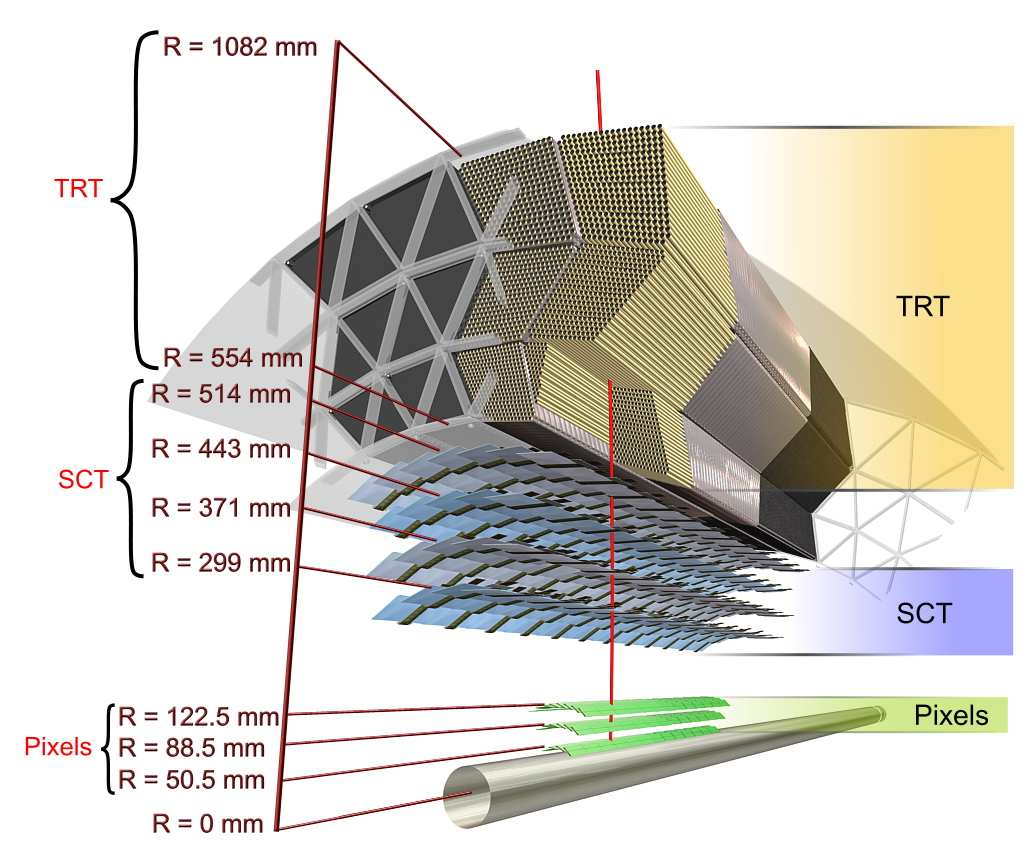
\includegraphics[scale=0.75]{images/image_inner_detector.jpg}
\caption{Illustration showing the path of a charged particle through the various layers of sub-detectors that make up the ID in the barrel region. The track passes the three cylindrical layers of the pixel layers, the four cylindrical double layers of the SCT, and finally around 36 axial straws. \cite{ATLAS}}
\label{inner}
\end{figure}
The ID is comprised of three distinct sub-detectors, with each using a different technology but all working in concert. The intrinsic resolutions of each of the sub-detectors in provided in table \ref{ID_res}. The sub-detectors with the best resoution are the precision tracking detectors: the pixel and silicon microstrip (SCT) detectors. The pixel detector is the more sensitive of the two, having 80.4 million readout channels to the SCTs' 6.3 million. It covers roughly the radial distance 50.5 mm to 150 mm from the beam-line and consists of 47 232 silicon pixels that are arranged in 1744 pixel modules. Around 90$\%$ of the pixels are $50 \mu m \times 400 \mu m$. Those remaining are slightly larger at $50 \mu m \times 600 \mu m$, these are specialised to cover the area between the chip boundaries of the pixel modules. The pixel modules themselves form three concentric barrels and two end-caps each with three discs. Usually a track coming from the interaction point will cross three pixel layers, subsequently resulting in three measurements. The pixels themselves have an adjustable threshold, any signal excess over which is considered a hit. In terms of its function, the pixel detector is essential in detecting the short-lived b-quarks and $\uptau$-leptons, and also contributes to the impact parameter measurement.
\begin{table}
	\centering{\begin{tabular}{|c|c|}
	\hline
	ID sub-detector & Intrinsic Resolution ($\mu m$) \\ \hline
	Pixel & 10($R$-$\phi$)115($z$) per sensor \\ \hline
	SCT & 17($R$-$\phi$)580($z$) per module \\ \hline
	TRT & 130 per straw \\ \hline
	\end{tabular}}
	\caption{Table listing the intrinsic resolution of each sub-detector of the ID. \cite{ATLAS}}
	\label{ID_res}
\end{table}

The SCTs cover roughly the radial distance from 299 mm to 560 mm from the beam-line. 4088 silicon-strip detector modules are formed into four concentric barrels and two end-caps, each of nine discs. They will register a hit if the pulse height exceeds a preset threshold of (usually) 1 femto Coulomb. The SCTs contribute to measurements of the momentum, impact parameter, and the corresponding vertex location from which the incident tracks originate. The SCT barrel modules are comprised of four rectangular silicon-sensor strips (two on each side), with the strips having a constant pitch of 80 $\mu m$. Two sensor at daisy chained together with a second pair being attached back-to-back with the first at a stereo angle of 40 mrad. Hence, the barrels are actually structured to be double-layered, such that a track originating from the beam-line results in eight measurements. Each of the end-cap disks is sub-divided into three rings. The modules in the middle and outer rings are formed in the same way as in the barrel, with two pairs of sensors being attached back-to-back at a stereo angle of 40 mrad. The modules of the inner ring are structured slightly differently and are made up of just two strips, attached back-to-back, at a stereo angle of 40 mrad. These two measurements per cylindrical barrel layer or disk, along with the stereo angle, are used to form discrete space-points, which are essential to the reconstruction of charged tracks in the ID (see section \ref{charged_reco}).

The Transition Radiation Tracker (TRT) covers roughly the radial distance 563 mm to 1066 mm from the beam-line. The TRT consists of 298 304 drift tubes, commonly referred to as straw-tubes, and 350 848 readout channels. The straw-tubes themselves are 4 mm in diameter and have a length of 1440 mm. The straw-tubes are filled with a gaseous mixture of Xe/CO$_{2}$/O$_{2}$ and in the centre of each straw-tube is a gold-plated tungsten wire. When a charged particle crosses the straw-tube, the gas-molecules become ionised. The central wire is positively charged and thus attracts the resulting free electrons (i.e. there is an anode wire inside a cathode tube). The subsequent charge spike on the anode constitutes a signal. This is amplified and read-out by electronics which register the fact that the straw-tube has been crossed. In terms of their geometrical layout, the straws in the barrel region form three concentric cylinders that lie parallel with the beam-axis. In the end-cap regions, the straw-tubes are orientated radially into 80 wheel resembling structures. Being the outermost of the three ID sub-detectors, the TRT deal with longer tracks and plays a significant role in measuring the momentum of those tracks.

Since it is the component of the ATLAS detector closest to the nominal interaction point, the sub-components of the ID (especially the innermost silicon pixel layers) need to be able to function even after prolonged exposure to a high-radiation environment. In fact, the cooling system of the ID must remove approximate 85 kW of heat from the ID volume at LHC design luminousity. The pixel and SCT detectors operate at a temperature of approximately -7$^{\circ}$C, while the TRT operates at room temperature.
\section{Calorimetry}
\label{calorimetry}
\subsection{Overview}
The ATLAS detector possesses a cutting-edge calorimetry system \cite{ATLAS} divided into two sub-detector systems: the Electromagnetic Calorimeter (ECal) and the Hadronic Calorimeter (HCal). Calorimeters are experimental devices used to measure an incident particle's energy. They are designed to cause the incident particle to initiate a particle shower (either electromagnetic or hadronic) and then measure the energy deposited in the calorimeter by containing the particle shower. Calorimeters are classified as either homogenous or sampling \cite{PDG}. In homogenous calorimeters, the entire volume is sensitive and contributes to the signal. In contrast, sampling calorimeters have alternating layers of absorber (dense material used to degrade the energy of the incident particle) and active medium which provides the detectable signal. Thus sampling calorimeters give an estimate of the energy of an incident particle since not all the energy is deposited in the active medium. This is in contrast to a homogenous calorimeter where the entire volume is sensitive and contributes a signal. Both the ECal and the HCal are examples of sampling calorimeters. They are both capable of energy measurements within a range of $| \eta | < 4.9$. As the names suggest, they rely on different physics interactions to function, with the ECal designed specifically for the containment of electromagnetic showers and the HCal for the containment of hadronic showers. Of the two, the ECal is the more sensitive (i.e. it has finer granularity) and is primarily concerned with measurements of electrons and photons. In contrast, the hadronic calorimeter is specialised to measure $E_{T}^{miss}$ and for jet reconstruction. It is possible for sufficiently high energy hadrons to ``punch through'' the HCal, where they can then be mistakenly reconstructed as muons in the muon spectrometer. The calorimetry system is shown in figure \ref{calorimeter}, while the granularity of each sub-detector is given in table \ref{granularity}.
\begin{figure}
\centering
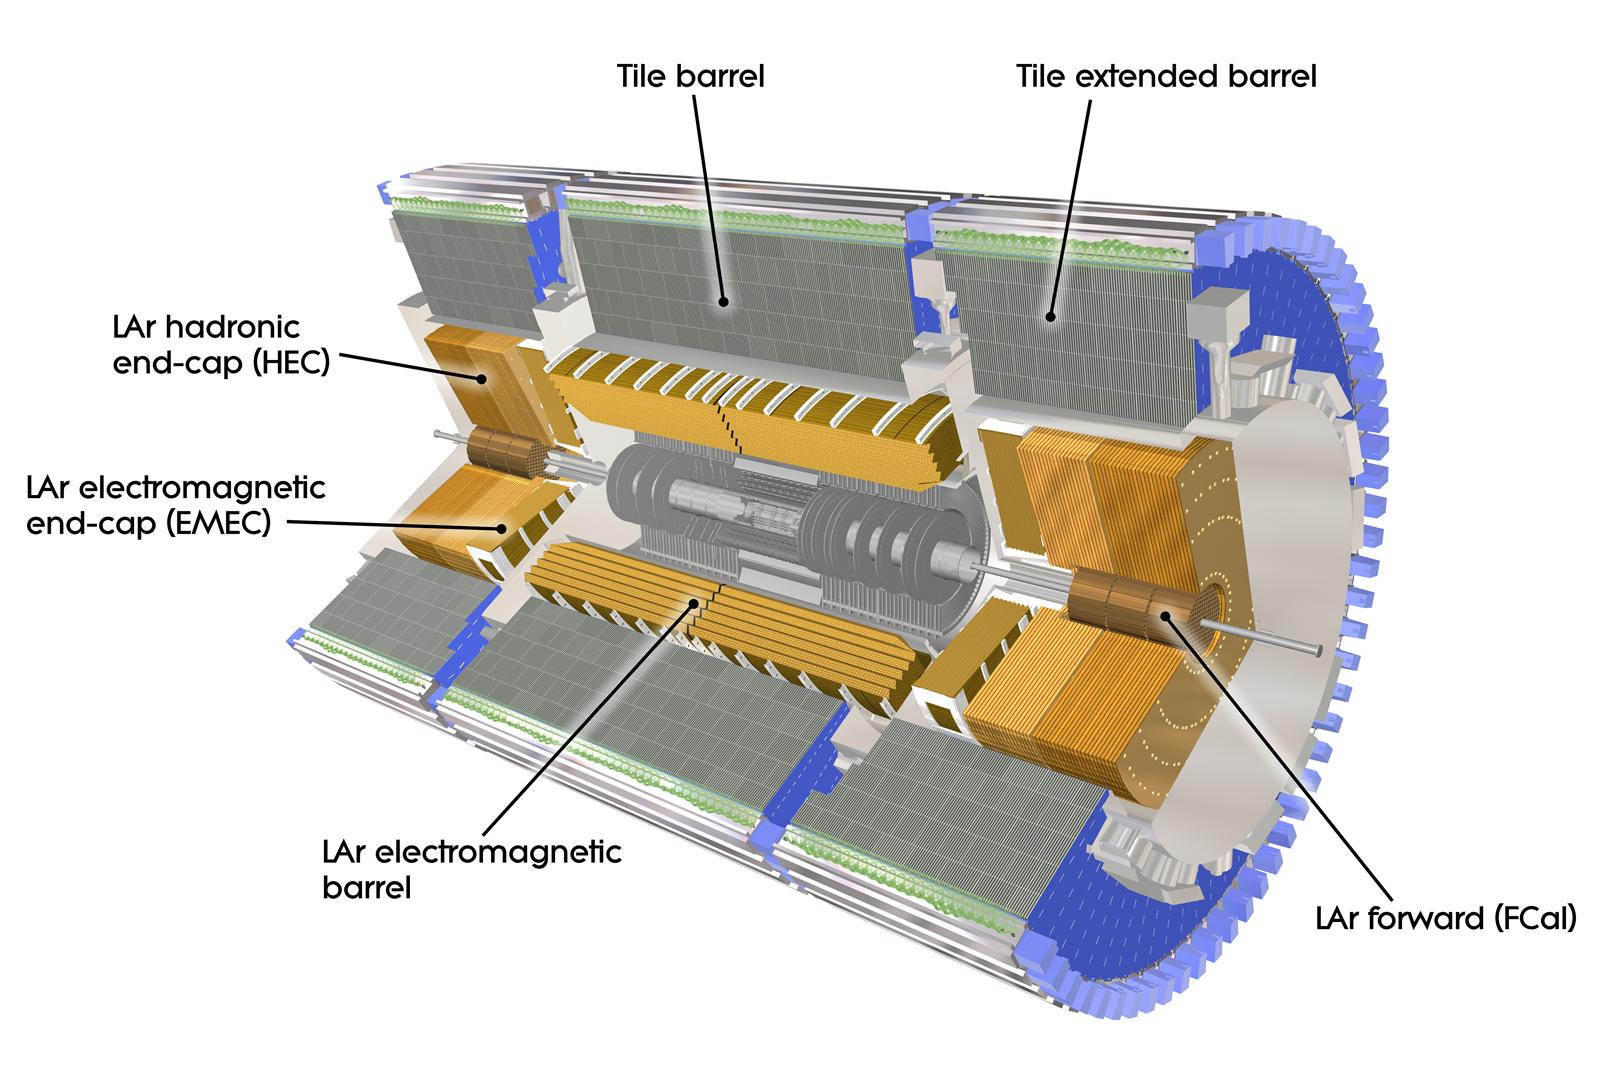
\includegraphics[scale=0.5]{images/image_calorimeter.jpg}
\caption{Illustration showing a cut-away view of the ATLAS detector's calorimetry system. \cite{ATLAS}}
\label{calorimeter}
\end{figure}
\subsection{LAr Electromagnetic Calorimeter}
The absorbers and electrodes of the ECal have an accordion geometry with full azimuthal coverage (i.e. there are no gaps, see figure \ref{accordion_design}) and pseudorapidity ranges of $| \eta | < 1.475$ for the barrel region and $1.375 < | \eta | < 3.2$ for the end-cap regions. It is divided into three layers with each layer segmented differently in $\eta$ and granularity (see table \ref{granularity}). It possesses 101760 readout channels in the barrel region, while it has 62208 in the end-cap region. The readout electrodes are located in the gaps between the absorbers and are comprised of three conductive copper layers, separated by insulating polyimide sheets. As the name suggests, the active medium is liquid argon (LAr) and, as a result, this calorimeter requires a cryostat in order to cool the system to its functioning temperature of -183$^{\circ}$C. Complementing the energy measurements provided by the ECal in the region $ | \eta | < 1.8$ is a separate thin liquid argon layer which forms the active medium for the presamplers. The presamplers serve to provide estimates of energy lost in front of the ECal. There are 7808 and 1536 readout channels in the presampler barrel and end-cap regions respectively. The active layer of LAr is 1.1 cm thick in the barrel region and 0.5 cm thick in the end-caps. Similarly to jets punching-through the HCal into the muon spectrometer, is possible for sufficiently high energy electrons or photons to pass into the hadronic calorimeter. In order to suppress this, the ECal is given a total depth of $> 33$ radiation lengths ($X_{0}$) in the barrel region and $> 24$ $X_{0}$ in the end-cap region. 

\begin{table}
	\resizebox{\textwidth}{!}{\centering{\begin{tabular}{|c|cc|cc|}
	\hline
	\textbf{Cal. Layer} & \multicolumn{2}{c|}{\textbf{Barrel}} & \multicolumn{2}{c|}{\textbf{End-Cap}}  \\ \hline
	 & Granularity ($\Delta \eta \times \Delta \phi$) & Coverage & Granularity ($\Delta \eta \times \Delta \phi$) & Coverage  \\ \hline
	 \multicolumn{5}{|c|}{\textbf{LAr Electromagnetic Calorimeter}} \\ \hline
	Presampler & $0.025 \times 0.1$ & $ | \eta | < 1.52$ & $0.025 \times 0.1$ & $1.5 < |\eta| < 1.8$  \\ \hline
	1st layer & $0.025/8 \times 0.1$ & $|\eta| < 1.40$ & $0.050 \times 0.1$ & $1.375 < | \eta | < 1.425$ \\
	 & $0.025 \times 0.025$ & $1.40 < | \eta | < 1.475$ & $0.025 \times 0.1$ & $1.425 < | \eta | < 1.5$ \\
	 & & & $0.025/8 \times 0.1$ & $1.5 < | \eta | < 1.8$ \\
	 & & & $0.025/6 \times 0.1$ & $1.8 < | \eta | < 2.0$ \\
	 & & & $0.025/4 \times 0.1$ & $2.0 < | \eta | < 2.4$ \\
	 & & & $0.025 \times 0.1$ & $2.4 < | \eta | <2.5$ \\
	 & & & $0.1 \times 0.1$ & $2.5 < | \eta | < 3.2$ \\ \hline
	 2nd layer & $0.025 \times 0.025$ & $| \eta | < 1.40$ & $0.050 \times 0.025$ & $1.375 < | \eta | < 1.425$ \\ 
	 & $0.075 \times 0.025$ & $1.40 < | \eta | < 1.475$ & $0.025 \times 0.025$ & $1.425 < | \eta | < 2.5$ \\
	 & & & $0.1 \times 0.1$ & $2.5 < | \eta | < 3.2$ \\ \hline
	 3rd layer & $0.050 \times 0.025$ & $| \eta | < 1.35$ & $0.050 \times 0.025$ & $1.5 < | \eta | < 2.5$ \\ \hline
	 \multicolumn{5}{|c|}{\textbf{Tile Calorimeter}} \\ \hline
	 All except last layer & $0.1 \times 0.1$ & & $0.1 \times 0.1$ & \\ \hline
	 Last layer & $0.2 \times 0.1$ & & $0.2 \times 0.1$ & \\ \hline
	 \multicolumn{5}{|c|}{\textbf{LAr Hadronic End-Cap Calorimeter}} \\ \hline
	 & & & $0.1 \times 0.1$ & $1.5 < | \eta | < 2.5$ \\ 
	 & & & $0.2 \times 0.2$ & $2.5 < | \eta | < 3.2$ \\ \hline
	 \multicolumn{5}{|c|}{\textbf{LAr Forward Calorimeter}} \\ \hline
	 & & & Granularity $\Delta x \times \Delta y$ (cm) & Coverage \\ \hline
	 1st module & & & $3.0 \times 2.6$ & $3.15 < | \eta | < 4.30$ \\
	 & & & $(3.0 \times 2.6)/4$ & $3.10 < | \eta | < 3.15$ \\
	 & & & & $4.30 < | \eta | < 4.83$ \\ \hline
	 2nd module & & & $3.3 \times 4.2$ & $3.24 < | \eta | < 4.50$ \\
	 & & & $(3.3 \times 4.2)/4$ & $3.20 < | \eta | < 3.24$, \\
	 & & & & $4.50 < | \eta | < 4.81$ \\ \hline
	 3rd module & & & $5.4 \times 4.7$ & $3.32 < | \eta | < 4.60$ \\
	 & & & $(5.4 \times 4.7)/4$ & $3.29 < | \eta | < 3.32$, \\
	 & & & & $4.60 < | \eta | < 4.75$ \\
	\hline
	\end{tabular}}}
	\caption{Table listing the granularity of each the sub-detectors of the calorimetry system. \cite{ATLAS}}
	\label{granularity}
\end{table}

\begin{figure}
\centering
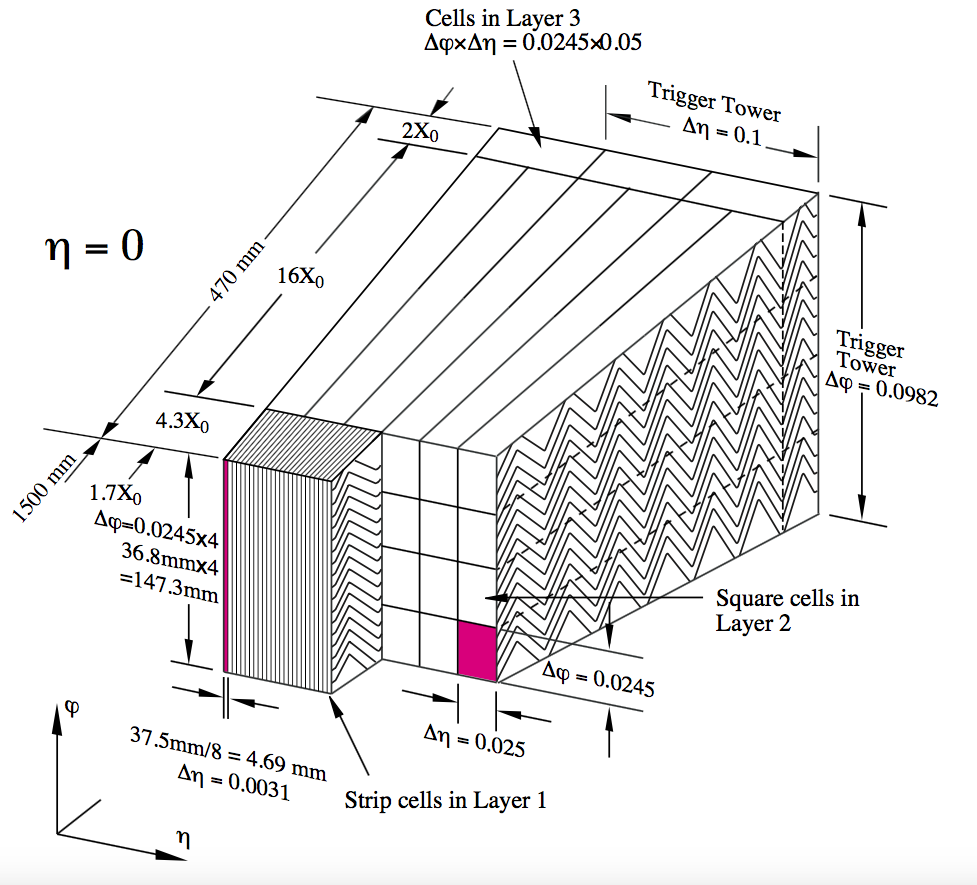
\includegraphics[scale=0.4]{images/accordion_design.png}
\caption{Illustration of an ECal barrel module showing its full azimuthal design. $X_{0}$ is the radiation length. \cite{ATLAS}}
\label{accordion_design}
\end{figure}
\subsection{Hadronic Calorimeters}
\subsubsection{Tile Calorimeter}
Enveloping the ECal is the Tile Calorimeter. It consists of three distinct structures: the barrel region, which covers the range $ | \eta | < 1.0$, and the two extended barrel regions which cover the range $ 0.8 < | \eta | < 1.7 $. As the name suggests, scintillating tiles form the active medium while steel is used as the absorber. The Tile Calorimeter occupies the annular volume defined by inner and outer radii of 2.28 m and 4.25 m respectively. It is radially segmented into three layers, while it is azimuthally segmented into 64 modules with a total of 5760 and 4092 readout channels in the barrel and end-cap regions respectively.
\subsubsection{LAr Hadronic End-Cap Calorimeter}
Located directly behind the end-cap ECal (and in fact sharing the same LAr cryostat), the LAr Hadronic End-cap Calorimeter (HEC) is comprised of two separate wheels. The HEC has a range of $ 1.5 < | \eta | < 3.2$ and does have some overlap with the Forward Calorimeter. Copper plates are used as the absorber, with the plates being interleaved with LAr which serves as the active medium. It has a total of 5632 readout channels.
\subsubsection{LAr Forward Calorimeter}
Integrated into the end-cap cryostat, the LAr forward calorimeter is divided into three modules (in each of the end-caps) with a total of 3524 readout channels. It provides hadronic calorimetry measurements in the extreme forward region, $3.1<|\eta|<4.9$. The first module consists of copper and is designed to primarily measure energy deposited through electromagnetic interactions. The other two consist of tungsten and are optimised for the measurement of energy deposited through strong interactions (hadronic showers). LAr is again used as the active medium.
\section{Muon Spectrometer}
The outermost sub-detector of the ATLAS detector is the Muon Spectrometer \cite{ATLAS}. It is designed to take muon measurements through the deflection of their tracks due to the magnetic field provided by its large superconducting air-core toroid magnets. It has approximately 1 million readout channels and occupies the annular volume defined by the inner and outer radii of 4.25 m (close to the calorimeter) and 11 m (the full radius of the ATLAS detector) respectively. The magnetic deflection is primarily due to the barrel toroid in the range defined by $ | \eta | < 1.4$, and primarily due to two smaller end-cap magnets inserted into each end of the barrel toroid for the range $1.6 < | \eta | < 2.7$. There is also a region $1.4 < | \eta | < 1.6$ where magnetic deflection is due to both, hence this is called the transition region. The Muon Spectrometer also possesses a separate trigger and high-precision tracking chambers. In the barrel region, these chambers are arranged in three cylindrical layers (parallel to the beam-axis) with radii 5m, 7.5 m, and 10 m from the beam-axis. The chambers in the transition and end-cap regions form wheel structures at $z \approx 7.4$ m, $10.8$ m, $14$ m, and $21.5$ m that lie orthogonal to the beam-axis.

There are four types of chambers found in the muon spectrometer. The Monitored Drift Tubes (MDTs) and Cathode Strip Chambers (CSCs) together form the precision-tracking chambers. They provide precise measurements of the track coordinate in the direction defined by the magnetic field. The MDTs cover the broad range $|\eta | < 2.7$. The CSCs provide additional tracking measurements for the forward region $2 < | \eta | < 2.7$ and are specially designed with higher granularity than the MDTs in order to cope with the high background rate in the forward region.

The other two chamber types: the Resistive Plate Chambers (RPCs) and Thin-Gap Chambers (TGCs) are used as part of the muon spectrometer's specialised muon trigger. The RPCs are used in the barrel, while the TGCs are used in the end-caps. These chambers cover the range $ | \eta | < 2.4$. The trigger chambers also play a role in measuring the muons' coordinates in the direction perpendicular to that measured by the precision-tracking chambers, as well as identifying the bunch-crossings from their resultant tracks.

\section{Forward Detectors}
The ATLAS forward region is covered by three small detectors \cite {ATLAS}. The first two, LUCID (LUminousity measurement using Cherenkov Integrating Detector) and ALFA (Absolute Luminousity For ATLAS), are located approximately 17 m and 240 m from the interaction point respectively. They are designed to measure the luminousity delivered to ATLAS. The third system ZDC (Zero-Degree Calorimeter) has an essential part in determining the centrality of heavy-ion collisions and is located approximately 140 m from the interaction point.
\section{Trigger System}
\label{trigger_system}
The ATLAS trigger system \cite {ATLAS} was briefly mentioned in section \ref{atlas_overview}. This section expands on that but is still only a brief overview. The ATLAS trigger system is divided into two distinct levels, namely, the hardware-based Level-1 (L1) Trigger \cite{l1_trigger} and the software-based High-Level Trigger (HLT) \cite{hlt}. The HLT refines the selections made by its predecessor and, when necessary, applies additional selection criteria. The L1 trigger uses only a small amount of the potentially available detector information in order to make a decision as to whether or not the event should be ignored or examined further. It makes this decision in a mean time of 2.5 $\mu$s per event, reducing the event rate from the 30 MHz proton-proton bunch crossing rate to 100 kHz. The L1 trigger makes this decision using important information from a sub-set of the sub-detectors. It searches for the high $p_{T}$ leptons, photons, and jets; as well as high missing transverse energy $E_{T}^{miss}$ or high total transverse energy $E_{T}^{tot}$. Calorimeter information is based off reduced granularity measurements in order to save time on the decision as to whether to keep the event. It also identifies Regions-of-interest (RoI) and passes this information onto the HLT. Using full granularity and precision, the HLT examines the RoI's with a mean event processing time of 200 ms, further reducing the event rate to 1 kHz. 
\chapter{Reconstruction and Identification of Physics Objects}
The primary reference for this chapter was \cite{ATLAS} and it should be consulted for further reading.
\section{Charged Particles in the Inner Detector}
\label{charged_reco}
The ID reconstructs the tracks of charged particles with $p_{T} > 0.5$ GeV and $ | \eta | < 2.5$ \cite{ATLAS}.  The track reconstruction is done in three steps:
\begin{enumerate}
\item Pre-Processing: Here raw data from the pixel detector is organised into groups of neighbouring triggered pixels called clusters. The clusters from the pixel-detector and the SCTs are converted into discrete space-points. The space-points for the SCT are calculated from the stereo angle of the SCT modules and the radial position for the barrel region and the longitudinal position for the end-cap regions. The space-points for the pixel-detector use only the radial (longitudinal) positions of the clusters to evaluate the corresponding space-points in the barrel (end-caps). The raw timing data from the TRT is converted into drift-circles, constructed using the radii defined by the minimum distance from the track to the wire in the straw-tube.
\item Track Finding: Here various track finding algorithms are implemented, the default of which uses the sensitive pixel and SCT detectors to locate tracks which can be traced back to the interaction point. Initially, combinations of space-points in the pixel detector and the first layer of the SCT detector are formed into track seeds. Next, the track seeds are extended out into the rest of the SCT layers, forming track candidates. Subsequently, some quality cuts are applied to the track candidates in order to reduce both the number of fake tracks and any ambiguities in relating specific tracks to clusters. Quality cuts will, for example, set limits on how many clusters may be shared between multiple tracks as well as the number of holes\footnote{A hole is defined as a sensor strip crossed by a track that generates no cluster.} permitted per track. As the track is extended into the TRT, it is matched to drift circles consistent with the extrapolation. The tracks are finally fitted with the full information available to the ID (i.e., information from each of the three sub-detectors) and compared against the silicon-only (pixel and SCT) track candidates. Poor comparison results in the candidate being classified as an outlier and removed.
\item Post-Processing: The primary vertex\footnote{In high-energy physics, the point where two particles collide in an accelerator is referred to as a vertex. During a bunch crossing in the LHC, it is likely that multiple proton-proton collisions will occur and hence often multiple vertices are reconstructed in each event. The vertex which possesses the largest sum of $p_{T}$ from its associated tracks is designated the primary vertex.} is reconstructed using a dedicated vertex finder before the reconstruction of photon conversions and secondary vertices.
\end{enumerate}
\section{Muons}
\label{muon_reco}
In practice, collisions at the LHC result in a wide spectrum of final-state muons. These range from low-momentum, non-isolated muons, such as those coming from $b$-jets, to high-momentum isolated muons, such as those coming from W/Z-boson decays \cite{ATLAS}.

The components of the ATLAS detector that are primarily responsible for the measurement of muons are the muon spectrometer and the inner detector, with the muon spectrometer being more effective for high momentum muons above a momentum threshold of 30 GeV and the inner detector being better suited for measuring muons with low to medium momenta. The muon spectrometer can, however, effectively detect and measure muons over a wide interval of energies and can trigger over $| \eta | < 2.4$.

In the momenta range from approximately 3 GeV to 3 TeV, muons are measured using three distinct but complimentary track reconstruction strategies:
\begin{itemize}
\item Stand-Alone: This is muon track reconstruction based only on the muon spectrometer data taken over the range defined by the spectrometer's acceptance of $| \eta | < 2.7$.
\item Combined: A combination of a muon spectrometer track with an inner detector track over the range defined by the inner detectors's acceptance of $ | \eta | < 2.5 $.
\item Segment\footnote{Track segments are defined as straight lines in a single MDT or CSC station and track candidates are reconstructed by fitting these segment together in layers.} Tag: This is a combination of an inner detector track with a muon spectrometer segment.
\end{itemize}
Track reconstruction within the muon spectrometer is logically divided into steps starting with the pre-processing of raw data to form drift circles in the MDTs, or clusters in the CSCs and the trigger chambers (RPCs and TGCs). This is followed by pattern-finding and segment making, segment combining, and finally track-fitting. This segment search and matching initially uses segments in the middle layers of the detector as seeds due to a relative abundance of hits there and then uses segments in the inner and outer layers as seeds. The track candidates are built from these matched segments. Combining segments from the muon spectrometer and the inner-detector is only possible in the region $|\eta | <2.5$, due to the geometrical acceptance of the inner-detector.
\section{Electrons and Photons}
Electrons and photons are reconstructed in the electromagnetic calorimeter and in the inner detector \cite{ATLAS}. The standard procedure is to start with seed-cluster. Electron and photon reconstruction is seeded using a sliding-window algorithm with the window size being $5 \times 5$ cells in the middle layer of the electromagnetic calorimeter. Fixed-size clusters are then reconstructed around the seed. The energy in the barrel electromagnetic calorimeter is measured over an area of $3 \times 7$ cells in the middle layer in the case of electrons and converted photons, and over an area of $3 \times 5$ cells for unconverted photons. For the end-cap electromagnetic calorimeters, both electrons and photons use an area of $5 \times 5$ cells. Attempts are then made to loosely match the clusters with one of the reconstructed tracks. Candidates are flagged if they appear to match to an apparent photon-conversion in the inner detector. Electron candidates are required to have a corresponding track but not be flagged for photon-conversion. Photon candidates are required to correspond to those seed-clusters that lack a matching track; or if they do have a track that it is flagged as originating from a photon conversion.
\subsection{Electrons}
\label{electron_reco}
Isolated high $p_{T}$ electrons are identified using a combination of cuts on the electromagnetic shower shapes, information from the reconstructed track, and the combined reconstruction. Three successively strict cut definitions can be applied in order to study electron candidates\footnote{Note that the cut definitions given here are summarised from \cite{ATLAS}. The reference should be consulted for the full definitions.}:
\begin{itemize}
\item Loose Cuts: These are basic cuts on the shower-shape and only require a very loose match between a given cluster in the calorimeter and the corresponding reconstructed track.
\item Medium Cuts: This adds additional cuts on the shower-shape using input from the first layer in the electromagnetic calorimeter and also applies cuts on track quality. These cuts include requiring that the track have at least seven hits in the pixel and SCT detectors and that the transverse and longitudinal impact parameters must have $| d_{0} | < 2$ mm and $| z_{0}-z_{v} | \times \sin\theta < 10$ mm respectively, where $z_{v}$ is the $z$-coordinate of the primary vertex and $\theta$ is the polar angle of the track.
\item Tight Cuts: Stricter track-matching is enforced in addition to imposing an energy-to-momentum ratio. Tight electrons also explicitly require a vertexing-layer (the innermost layer of the pixel-detector) hit on the track to further clean out photon conversions and additionally require a high ratio between high-threshold and low-threshold hits in the TRT detector. This latter requirement reduces background resulting from charged hadrons.
\end{itemize}
\subsection{Photons}
Photons are identified using an equivalent set of cuts to those defined for electrons. The photon cuts have, however, been optimised based on shower-shapes in the calorimeter, with particular attention to using the fine granularity of the strip layer in order to reduce background from single $\pi^{0}$'s. $\pi^{0}$'s are further excluded by utilising track isolation requirements. Such requirements give an efficiency of 84$\%$ for photons coming from the $H \longrightarrow \gamma \gamma$ channel, assuming a Standard Model Higgs with $m_{H} = 120$ GeV. The efficiency is approximately constant across the $\eta$ range, with an exception being located at the crack between the barrel and the end-caps.
\section{Jets}
The primary resource for the writing of this section was \cite{ryan}.

QCD calculations are performed in terms of the final state quarks and gluons. After hard scattering occurs, quarks and gluons will follow a branching process and then subsequently hadronise. The result is a collimated grouping of hadrons which is what is referred to as a QCD jet. In order to compare theoretical predictions with data, a way of mapping the  final state hadrons observed in our detector to partons resulting from a hard scatter is needed. This mapping is what is referred to as the \emph{jet algorithm}. It is also necessary to have a structured way to assign four-momenta to particles within a jet, which is called the \emph{recombination scheme}. Taken together the jet algorithm and recombination scheme determine what we call the \emph{jet definition}. Such definitions are required to posses a variety of properties which will not be listed here but suffice to say they must be ``well-behaved''. A jet algorithm that avoids being dependent on the unknown, long-distance properties of QCD where perturbation theory breaks down is said to be \emph{infrared safe}. ATLAS has two default jet reconstruction algorithms \cite{ATLAS}: seeded fixed-cone algorithms and successive recombination algorithms. Seeded fixed-cone algorithms will be discussed first.

Seeded fixed-cone algorithms attempt to reconstruct a jet by defining a cone centred on a given point, referred to as the seed. Seeded fixed-cone algorithms rely on two parameters, namely the transverse energy $E_{T}$  threshold for a given seed, and the cone size $\Delta R = \sqrt{\Delta y ^{2} + \Delta \phi ^{2}}$. These algorithms are fairly easy to implement but are not however infrared safe.

Sequential recombination algorithms are based around having some measure of how likely it is that two partons arose from the same QCD splitting. The jet is then sequentially constructed by reconstructing the partons which are closer in this measure. The most basic form of this algorithm is the \emph{inclusive $k_{t}$ algorithm}. For two particles $i$ and $j$, define the following distance:
\begin{eqnarray}
\label{d_ij}
d_{ij} & \equiv & min\left( p^{2}_{\mathbf{T},i};p^{2}_{\mathbf{T},j} \right) \frac{\Delta R_{ij}^{2}}{R^{2}},
\end{eqnarray}
where $R$ is the radius of the jet and $\Delta R_{ij}^{2}  \equiv  \left( y_{i} - y_{j}\right)^{2} + \left( \phi_{i} - \phi_{j} \right) ^{2}$. Define also, the distance from a particle $i$ to the beam \textbf{B} as:
\begin{eqnarray}
\label{d_iB}
d_{i \mathbf{B}} & \equiv & p_{\mathbf{T},i}^{2}.
\end{eqnarray}
The algorithm then works as follows:
\begin{enumerate}
\item For all final state particles, determine all the distances between each particle to all other particles (using \ref{d_ij}) and the distances from each individual particle to the beam (using \ref{d_iB}).
\item Find the minimum of all these distances.
\item If the mimium distance is between two particles, then recombine the particles in question and go back to the first step.
\item Otherwise if it is betweem a particle and the beam, then declare the particle to be a jet and remove it from the list of particles. Back to step 1.
\item Terminate the algorithm when no particles remain.
\end{enumerate}
Actually, the $k_{T}$ algorithm can be generalised as follows:
\begin{eqnarray}
d_{ij} & \equiv & min\left( p^{2p}_{\mathbf{T},i};p^{2p}_{\mathbf{T},j} \right) \frac{\Delta R_{ij}^{2}}{R^{2}} \\
d_{i \mathbf{B}} & \equiv & p_{\mathbf{T},i}^{2p}.
\end{eqnarray}
The advantage of all sequential recombination jet algorithms over seeded fixed-cone algorithms is that they are all infrared safe. Some common values for $p$ are:
\begin{itemize}
\item $p = 1 \longrightarrow$ inclusive $k_{T}$ algorithm \cite{kt}
\item $p = 0 \longrightarrow$ Cambridge/Aachen \cite{cambridge-aachen}
\item $p = -1 \longrightarrow$ Anti-$k_{T}$ algorithm \cite{anti-kt}
\end{itemize}
In practice the Anti-$k_{T}$ algorithm is preferred over the inclusive $k_{T}$ algorithm as the computational time $T$ for the latter is $T= \mathcal{O}\left(N^{3}\right)$ while for the \emph{FastJet} \cite{fastjet} implementation of the former $T = \mathcal{O}\left(N \ln {N}\right)$.
\section{Missing Transverse Energy}
The primary reference for writing this section was \cite{pizio_thesis} and should be consulted for further reading.

Transverse momentum $p_{T}$, is the momentum of an object transverse to the beam. The initial longitudinal momentum in a parton collision is unknown, because the partons that make up a proton share some fraction of the proton's momentum (Bjorken $x$). In contrast, the initial transverse momentum of the colliding partons is known to be zero. Searching for missing transverse momentum, defining: $$p_{T}^{miss} = - \sum_{i} p_{t}(i)$$ for visible particles, can thus be indicative that new, unaccounted for, particles have escaped the detector. Transverse energy for an object is defined as $E_{T} = \sqrt{m^{2} + p^{2}_{T}}$, where $m$ is its invariant mass and $p_{T}$ its transverse momentum. In practice, it is rather the missing transverse energy that is reconstructed rather than the transverse momentum, but its measurement can similarly be to infer the existence of otherwise  undetected particles. Hence, $E_{T}^{miss}$ is essential in the detection of neutrinos and in the search for physics beyond the Standard Model.

In the ATLAS detector, the reconstruction of missing transverse energy comes from reconstructed energy deposits in the calorimetry system, and from reconstructed muon tracks. It is important to note that energy deposits and muon tracks can arise from sources other than the hard scattering process, e.g. the underlying event, pile-up, and cosmic rays.

Initially, the algorithm applies a noise suppression procedure and subsequently identifies calorimeter cells that still indicate the presence of an energy deposit. These cells are calibrated using their global calibration weights (dependent on their energy density) as described in \cite{ATLAS}. Since this initial step does not yet rely on other reconstructed objects, it is fairly robust, even during initial data taking \cite{pizio_thesis}. The cells are then calibrated according to the reconstructed object they correspond to. Corrections are applied to account for the energy lost due to muons escaping (though detected by) the detector, as well as for the energy lost in the cryostat between the LAr electromagnetic and tile calorimeters.

The missing transverse energy can be resolved into $x$ and $y$ components:
\begin{equation}
E_{T}^{miss} = \sqrt{\left( E_{x}^{miss} \right)^{2} + \left( E_{y}^{miss} \right)^{2}}.
\end{equation}
These components include sub-terms for the transverse energy deposited in the calorimeter, as well as corrections for the energy lost in 1) the cryostat and 2) due to muons. The $x$ and $y$ terms can thus be written as:
\begin{equation}
E_{x,y}^{miss} = E_{x,y}^{miss,calo} + E_{x,y}^{miss,cryo} + E_{x,y}^{miss,\mu}.
\end{equation}
The calorimeter terms can be written as:
\begin{eqnarray}
E_{x}^{miss} &=& - \sum_{i=1}^{N_{cells}} E_{i} \sin \theta_{i} \cos \phi_{i}, \\
E_{y}^{miss} &=& - \sum_{i=1}^{N_{cells}} E_{i} \sin \theta_{i} \sin \phi_{i},
\end{eqnarray}
where $E_{i}$, $\theta_{i}$, and $\phi_{i}$ are the cell's energy, polar angle, and azimuthal angle respectively. Due to the high granularity of the calorimetry system (see section \ref{calorimetry}), it is necessary to implement some kind of noise suppression. This is done by limiting the number of cells, $N_{cells}$, in the summations. This can be done, practically, by only counting cells belonging to topoclusters (see section \ref{calorimetric_isolation} for more information on topoclusters and how they are built).

The muon term is calculated from the momenta of the muons measured:
\begin{equation}
E_{x,y}^{miss,\mu} = - \sum_{selected \ muons} E_{x,y}^{\mu}.
\end{equation}
In the region $|\eta | <2.5$, only good quality muons in the muon spectrometre, with a matched track in the ID, are considered. This is to reduce contributions from fake muons. For muons that lie within $2.5 < | \eta | < 2.7$ (outside the acceptance of the ID), there is no matched track requirement. Some energy is lost by those muons that pass through small regions not covered by the muon spectrometre. This energy can be recovered using muon information from the ID and calorimetry system.

For further reading, please see the references for the two reconstruction methods used by ATLAS, \verb!STACO! \cite{STACO} and \verb!MuID! \cite{MuID}.
\section{$b$-jet Tagging}
Tagging jets that originate from heavy flavour quarks is useful for many physics analyses. Briefly described here is the tagging of jets that specifically originate from $b$-quarks. A jet is labelled by definition as a $b$-jet if it originated from a  $b$-quark with $p_{T} > 5$ GeV. Similarly a $c$-jet (or $\uptau$-jet) is labelled by definition as such when it originates from a $c$-quark ($\uptau$-lepton) with $p_{T} > 5$ GeV. Jets that do not originate from heavy quarks or $\uptau$-leptons are labelled \emph{light jets}.
\subsection{Basic $b$-Tagging Algorithms}
ATLAS has three basic $b$-tagging algorithms that output discriminating variables that independently help in differentiating jet flavours \cite{valerio_on_btagging}:
\begin{itemize}
\item Impact Parameter Based Algorithm
\item Inclusive Secondary Vertex Reconstruction Algorithm
\item Decay Chain Multi-Vertex Reconstruction Algorithm.
\end{itemize}
Since the output discriminating variables are obtained by separate independent means in each basic algorithm, they can be used together as input for a so-called multivariate discriminant (see \ref{mva}). All three basic algorithms have the preliminary step of track selection.
\subsubsection{Track Selection}
This step serves to reject fake tracks and gives some measure of how precisely a given track is matched to a jet. Tracks are matched to jets in the calorimeter through $\Delta R$ matching, taking into account that higher $p_{T}$ jets tend to result in narrower, more collimated cones. So a $p_{T} = 20$ GeV jet requires a track be within $\Delta R = 0.45$, while a higher $p_{T}$ jet of 150 GeV requires that a matching track be found within $\Delta R = 0.26$ \cite{b_tagging_extra}. Any ambiguity introduced by multiple tracks meeting the $\Delta R$ criterion is resolved by then selecting the closest track in $\Delta R$. Quality cuts are then applied to the matched tracks. These quality requirement are dependent on which algorithm is being used.

Impact parameters used in impact parameter based algorithms are the transverse impact parameters and the longitudinal impact parameters. The transverse impact parameter $d_{0}$ is defined as the shortest path between the track and the primary vertex in $r-\phi$ space. The z-coordinate at this point is defined as the longitudinal impact parameter $z_{0}$. The quantity $d_{0}/\sigma_{d_{0}}$, where $\sigma_{d_{0}}$ is the uncertainty in $d_{0}$, is called the transverse impact parameter significance. It is used in order to give more weight to more precisely measured tracks. Critical track quality requirements include $p_{T} > 1$ GeV, $|d_{0}| < 1$ mm, $|z_{0} \times \sin \theta  | < 1.5 $ mm, and a minimum of two pixel detector hits.

Secondary vertex based algorithms use a looser track quality requirement as the additional reconstruction of the secondary vertices places less emphasis on the track quality for efficiency.
\subsubsection{Impact Parameter Based Algorithm}
There are two impact parameter based algorithms used by ATLAS: IP2D \cite{IP?D} and IP3D \cite{IP?D}, with the latter using both the longitudinal and transverse impact parameters and the former only using the transverse impact parameter. IP2D is, however, less sensitive to the complicating effects of pile-up. Both use the signed impact parameter significance of the matched tracks. If the closest path between a given track and the primary vertex is in front of the Primary Vertex with respect to the jet direction, then the impact parameter is signed positive. The converse is then signed negative. Ratios are defined for the $b$- and light-jet hypotheses using the Probability Density Functions (PDFs) of the signed impact parameter significance of the tracks. These are merged into a single log likelihood discriminant (LLR) which can then be used to discriminate between jet-flavours.
\subsubsection{Secondary Vertex Finding Algorithm}
This algorithm attempts to differentiate jet flavours based on the properties of reconstructed secondary vertices from within the jet. Secondary vertex candidates are required to have at least two tracks associated with them. To help ensure the secondary vertex originates from within a jet, tracks likely from photon conversions, hadronic interactions with detector material, or from the decays of long-lived particles (e.g. $K_{S}$ or $\Lambda$) are excluded. 
\subsubsection{Decay Chain Multi-Vertex Algorithm: JetFitter}
JetFitter \cite{jetfitter} attempts to reconstruct the full primary vertex $\rightarrow b \rightarrow$ $c$-hadron decay chain through its topological structure. The connecting line between the primary vertex an the bottom and charm vertices is found using a Kalman Filer, estimating the positions and paths of the $b$-hadrons. This powerful approach allows for resolution of $b$- and $c$-hadron vertices even when only a single track is associated with them. 
\subsection{Multivariate Algorithm}
\label{mva}
The output discriminating variables from the three basic algorithms can be used together as input into the ATLAS Run 2 multivariate algorithm \cite{b-tagging_ref}. This is a boosted decision tree (BDT) algorithm, trained on five million $t\bar{t}$ events. It is the successor to the previous ATLAS Run 1 multivariate algorithm \cite{MV1}, which was a neural network algorithm. The multivariate algorithm is trained by assigning a background mixture of 10$\%$ $c$-jets and 90$\%$ \emph{light}-jets. The discriminating variables from IP2D, IP3D, Secondary Vertex Finder, and JetFitter, together with the jet kinematics are provided as input. Cuts on the multivariate algorithm output distribution define the $b$-jet efficiency, which serve as the working points for the $b$-tagger. The working points are shown in table \ref{b-tagger_working_points}, along with the rejection rates of other jet-flavours.
\begin{table}
	\begin{tabular}{|c|c|c|c|c|}
	\hline
	 \emph{b}-jet Efficiency [$\%$] & \emph{c}-jet Rejection & $\uptau$-jet Rejection & Light-jet Rejection \\ \hline
	60 & 34.54 & 183.98 & 1538.78 \\
	70 & 12.17 & 54.72 & 381.32 \\
	77 & 6.21 & 22.04 & 134.34 \\
	85 & 3.10 & 8.17 & 33.53 \\ \hline
	\end{tabular}
	\caption{Working points for the multivariate algorithm with the benchmarking efficiency and rejection rates. \cite{b-tagging_ref}}
	\label{b-tagger_working_points}
\end{table}
\section{Isolation}
\label{isolation_section}
Isolation is a measure of the numbers of particles produced in a cone in $\eta - \phi$ space, defined by $\Delta R$ , around the detector signature corresponding to the reconstructed lepton. These cones are categorised according to their size, so a cone with $\Delta R = 0.2$ is forms part of the \textbf{cone20} classification. Similarly, cones with sizes $\Delta R=0.3$ and $\Delta R =0.4$ are categorised into the \textbf{cone30} and \textbf{cone40} classifications respectively. Since hadrons are often produced in collimated flows (called jets), fake leptons are less likely to be isolated when compared to prompt leptons. Thus lepton isolation can be used to reduce the fake lepton background.

Isolation variables generally fall into two categories: those determining the isolation energy using the tracker and those using the calorimeter. These result in two separate classes of variables which are usually used in complement. Variables derived from tracker information have the advantage of being fairly resistant to the effects of pile-up, while those from calorimeter information can be applied to neutral hadrons.
\subsection{Calorimetric Isolation}
\label{calorimetric_isolation}
The variable \textbf{etcone} is simply the sum of all the transverse energy in all calorimeter (both electromagnetic and hadronic) cells that lie within the isolation cone centred on the lepton/photon. However, this variable proved to be susceptible to the effects of pile-up and had poor data-MC agreement in Run 1 \cite{laplace}. Another, preferable, variable is \textbf{topoetcone}. Instead of summing the transverse energy of all cells within the cone, \textbf{topoetcone} only sums the contributions coming from topological clusters whose barycentre lies within the isolation cone.

Topological clusters \cite{laplace_21} are clusters that are seeded by cells which have an energy that exceeds its noise threshold by at least a factor of four. This is the barycentre of the cluster; it is expanded by adding any neighbouring cells with an energy of at least a factor of two above the noise threshold. Once the cluster can expand no further in this manner, a final layer of cells is added and the cluster is fully defined. The topological clusters used in the isolation computation are not further calibrated, remaining at the electromagnetic scale.

The direction is determined differently for electrons/photons and muons. The electron/photon direction comes from the position of the rectangular calorimeter cluster used in the reconstruction of the electron's/photon's energy. On the other hand the muon direction is determined by the weighted mean of the extrapolated positions of the muon track in the electromagnetic calorimeter.

The sum of all positive energy contributions from topological clusters whose barycentre lies within the isolation cone is defined as the raw \textbf{topoetcone} isolation $E_{T, raw}^{isol}$. This is shown in figure \ref{topo_clusters}.

The raw \textbf{topoetcone} isolation as defined above still includes the core energy of the original lepton/photon. In practice this is subtracted from the final isolation variable. The way this energy is subtracted can vary but the default core subtraction technique for electrons and photons is the \textbf{core57cells}. In this technique, cells in a $5 \times 7$ rectangle around the barycentre are not considered in the energy calculation. The \textbf{coreMuon} technique is instead used for muons. Here the muon energy is summed in optimally sized fixed windows in each calorimeter layer and then subtracted. These core corrections are denoted $E_{T, core}$.

The default electron and photon \textbf{core57cells} subtraction technique is imperfect and some energy from the electron/photon inevitably will leak into the isolation cone. This requires additional subtraction to compensate, the so-called leakage correction, denoted $E_{T, leakage}$. The details of determining the leakage correction are outside the scope of this thesis. Suffice to say, it is an estimated average using MC samples of single electrons and photons, assuming no pile-up \cite{laplace}.

Fianlly for electrons, photons, and muons, a pile-up correction is estimated from the size of the isolation cone and the energy density of the event (calculated using the energy density of each jet in an event) using the \emph{FastJet} \cite{laplace_22} package. This correction is denoted $E_{T, pile-up}$.

The final correction \textbf{topoetcone} isolation for electrons and photons is:
\begin{equation}
\mathbf{topoetcone} = E_{T, raw}^{isol} - E_{T, core57cells} - E_{T, leakage} - E_{T, pile-up},
\end{equation}
and for muons:
\begin{equation}
\mathbf{topoetcone} = E_{T, raw}^{isol} - E_{T, coreMuon} - E_{T, pile-up}.
\end{equation}
\subsection{Track Isolation}
\textbf{ptcone} is calculated by summing the transverse momenta of tracks that lie within the isolation cone centred around the lepton track or photon direction. Only tracks that pass selection cuts on $p_{T}$ and $| z_{0} \sin\theta |$ are summed. The $p_{T} > 1$ GeV cut is used to suppress the fake lepton background while the $| z_{0} \sin \theta | < 3$ mm cut is designed to minimise pile-up interference by selecting for tracks that are likely coming from the primary vertex.

A modified version of \textbf{ptcone} with a variable cone size \textbf{ptvarcone} can be used instead. With this variable, the cone size shrinks as the $p_{T}$ of the lepton or photon increases. The cone size is determined according to 
\begin{equation}
\Delta R = \min \left( \frac{k_{T}}{p_{T}},R \right),
\end{equation}
where $k_{T}$ is a constant set to 10 GeV and $R$ is the maximum cone size (ranging from 0.2 to 0.4). Because of the varying cone size, \textbf{ptvarcone} is better suited to handle boosted signature or busy events in which other objects can end up near the lepton or photon direction.

In an analogous case to calorimeter isolation, in track isolation the track of the lepton or photon is subtracted from the final variable. This is handled differently for electrons, muons, and photons.
\begin{itemize}
\item for muons: the corresponding track is removed
\item for converted photons: any corresponding tracks (unconverted photons do not contribute to track isolation)
\item electrons are more difficult to handle due to Bremsstrahlung. The procedure involves extending relevant tracks into the calorimeter and counting those that fall into a $\eta - \phi$ window around the electron cluster. This is described in detail in \cite{laplace_23}.
\end{itemize}
\begin{figure}
\centering
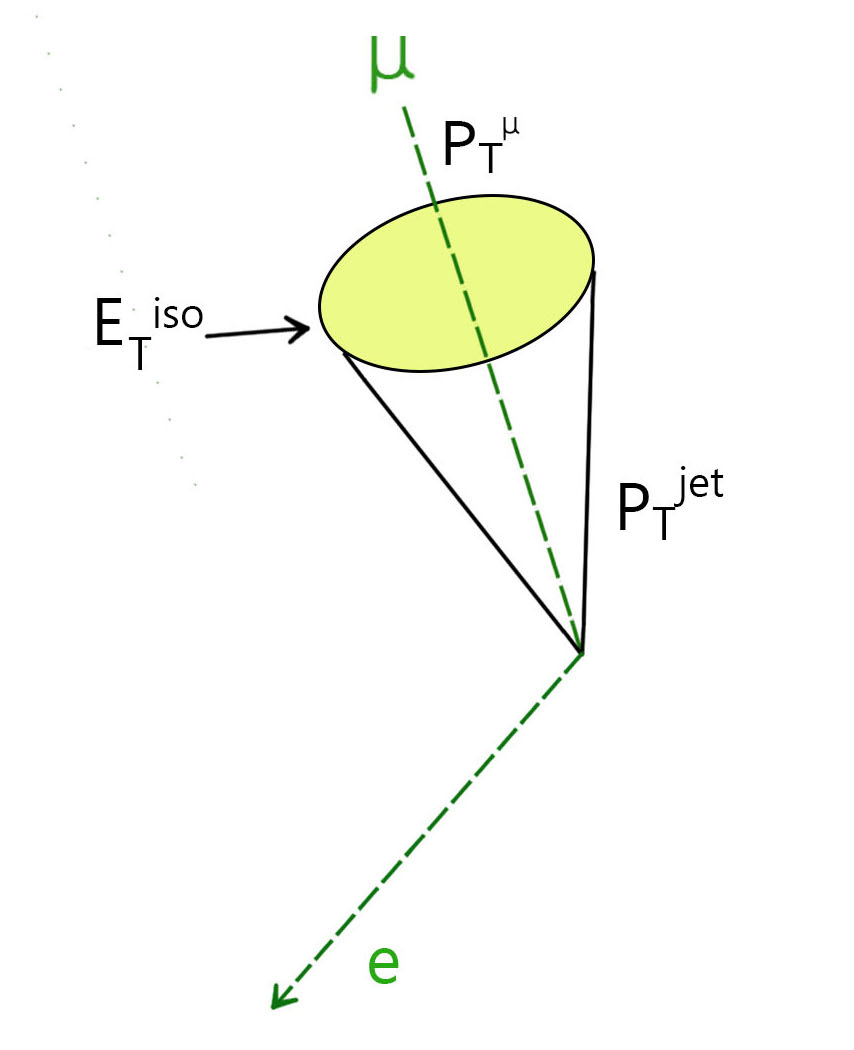
\includegraphics[scale=0.2]{images/iso_cone.jpg}
\caption{An illustration of an event where a prompt electron and a non-prompt muon, coming from a jet, fake a same-sign W-boson scattering event. Since the non-prompt muon is from a jet it is less likely to be isolated than than if it were prompt. Modified from \cite{ssWW_int_note}.}
\label{isolation_cone}
\end{figure}

\begin{figure}
\centering
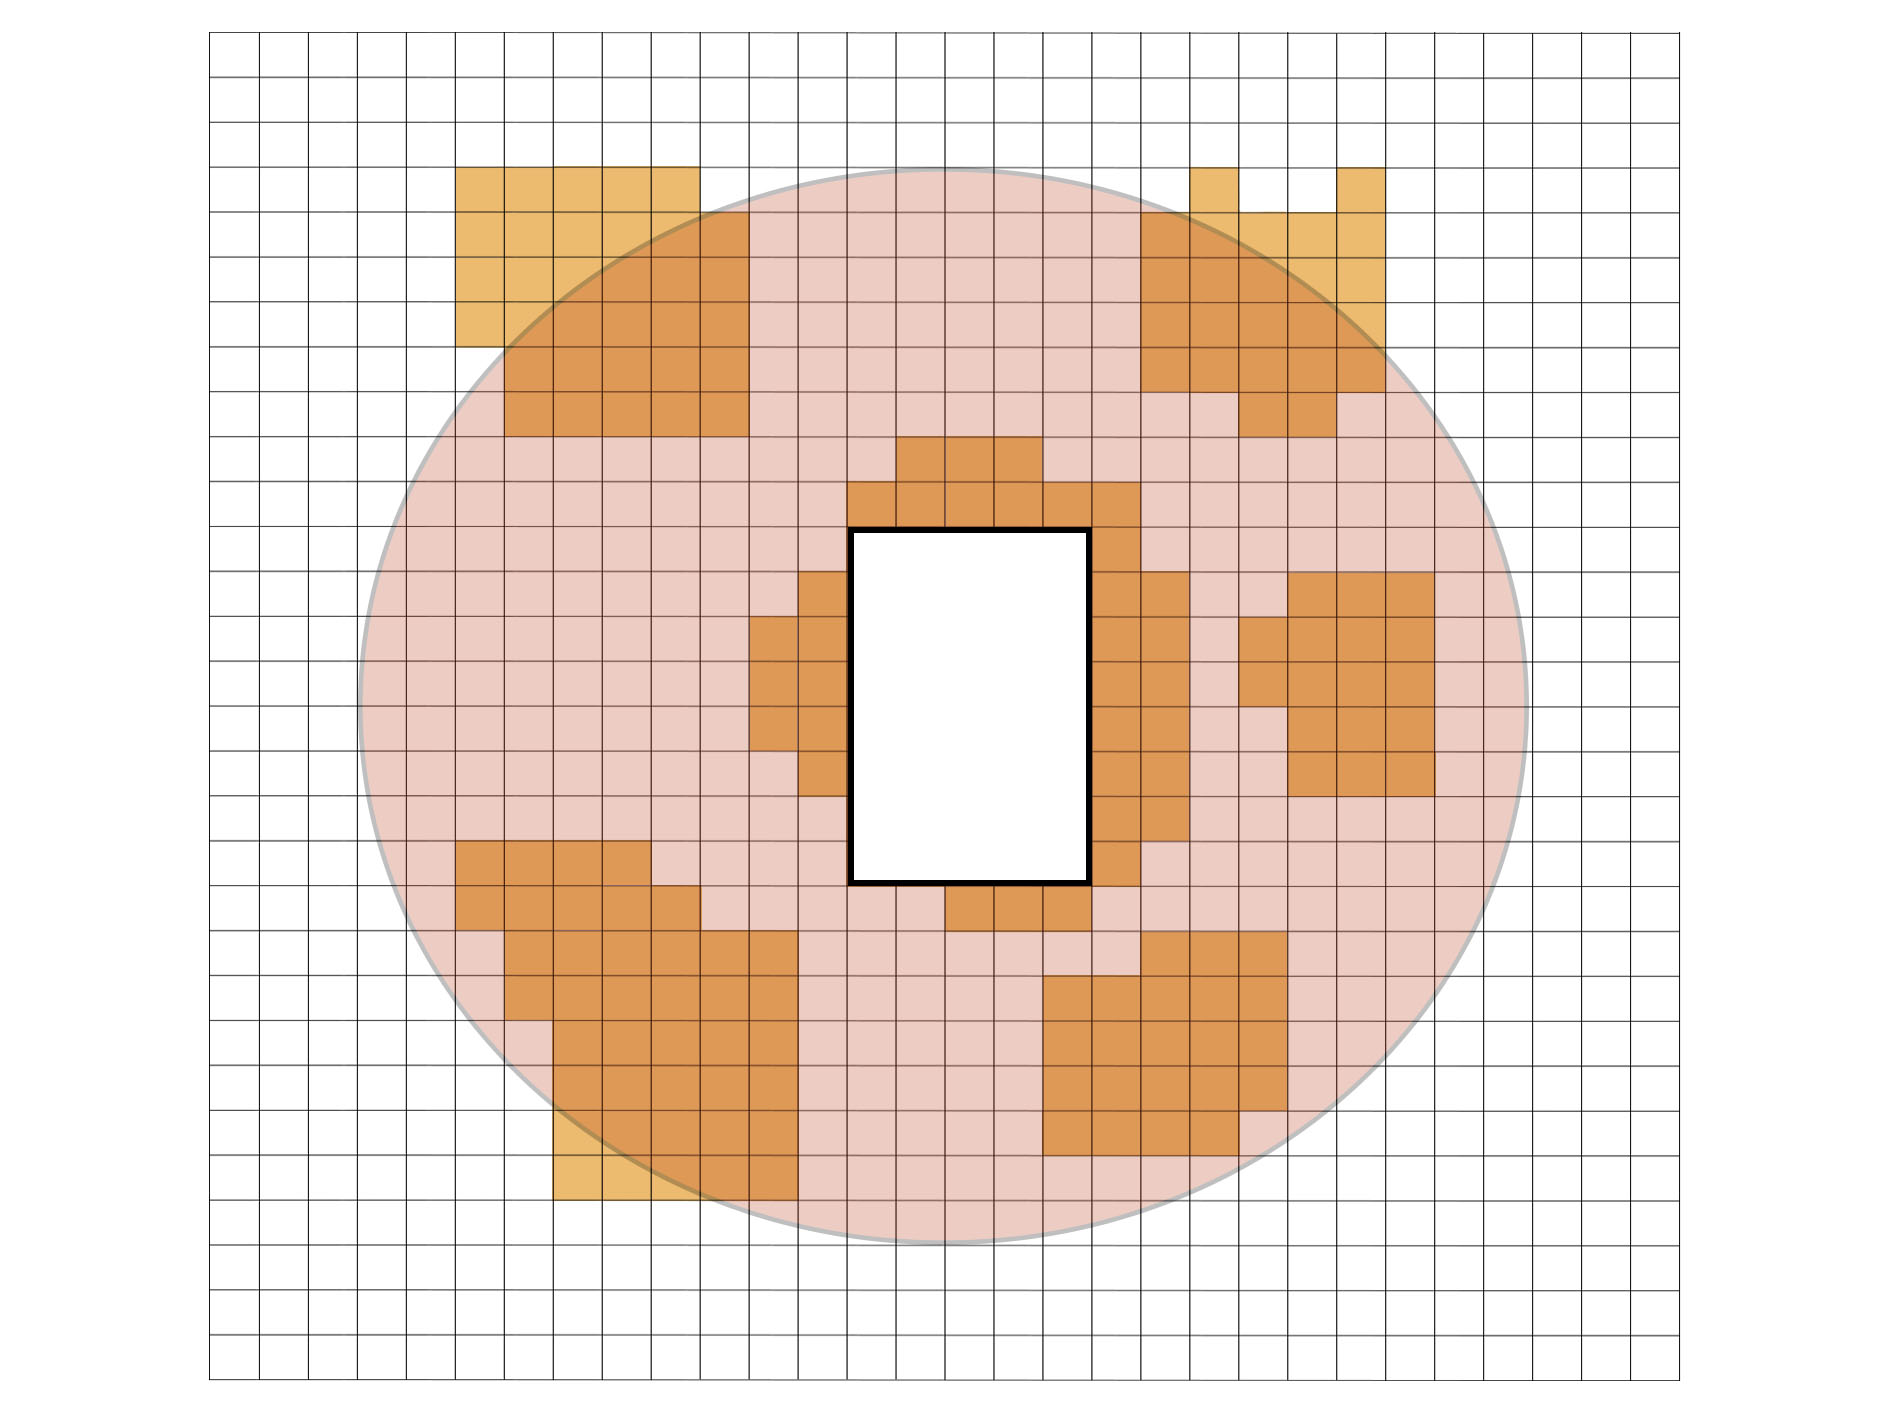
\includegraphics[scale=0.65]{images/topo_clusters.jpg}
\caption{An illustration of how the \textbf{topoetcone} variable is constructed. The grid in $\eta - \phi$ space represents the middle calorimeter cells. At the centre of the cone lies the incident lepton/photon. The topological clusters (coloured orange) are included in the calculation if their barycentre lies within the cone. The white $5 \times 7$ rectangle represents the cells subtracted in the calculation when using the \textbf{core57cells} technique. Modified from \cite{laplace}.}
\label{topo_clusters}
\end{figure}
\subsection{The ATLAS Isolation Selection Tool Working Points}
\label{AIST}
The isolation working points should be as independent of event topology as possible. Thus they are based on isolation variables using the smallest cone size $\Delta R = 0.2$, and for lepton track isolation \textbf{ptvarcone}. Motivated by this, the working points are based on the \textbf{topoetcone20} and \textbf{ptvarcone20} variables.
The official \emph{ATLAS Isolation Selection Tool} posses a number of official working points which can be used to accept or reject leptons with varying degrees of efficiency. The efficiency is defined, in the context of $Z \longrightarrow \ell \ell$ ($\ell = e/\mu$), as
$$\varepsilon =  \frac{N_{e/\mu}^{pass}}{N_{e/\mu}^{all}}, $$
where $N_{e/\mu}^{pass}$ is the number of electrons/muons originating from the hard process that pass the isolation requirement, while $N_{e/\mu}^{all}$ is the total number of electron/muons originating from the hard process. The process, $Z \longrightarrow \ell \ell$, is chosen due to its clean experimental signature.

These official working points can be classified as either:
\begin{itemize}
\item simple fixed cuts of the from $\mathbf{ptvarcone30} < X$ GeV,
\item so-called targeted efficiencies, with either gradient efficiency of 95$\%$ at $p_{T} = 20$ GeV and 99$\%$ at $p_{T} = 80$ GeV or flat efficiency of 99$\%$ in the $\eta-\phi$ plane. These lepton only working points are based on cut maps from $Z \longrightarrow \ell \ell$ Monte Carlo samples.
\end{itemize}
Many fixed cuts are applied to the fractional isolation (the isolation variable divided by $p_{T}$). These cuts are useful in that they are looser on high $p_{T}$ leptons and hence suited to searches for high $p_{T}$ objects. Only fixed isolation cuts are applied to photons.
Some example isolation working points are described in table \ref{iso_wps}.
\begin{table}
	\resizebox{\textwidth}{!}{\centering{\begin{tabular}{|c|c|c|c|c|}
	\hline
	Working Point & Objects & Calorimeter Isolation & Track Isolation & Combined Isolation \\ \hline \hline
	\textit{Loose} & all leptons & 99$\%$ & 99$\%$ & 99$\%$ \\ \hline
	\textit{Gradient} & leptons & $\varepsilon$=(0.1143$\times$$p_{T}$[GeV]+92.14)$\%$ & $\varepsilon$=(0.1143 $\times$$p_{T}$[GeV]+92.14)$\%$ & $\varepsilon$(25 GeV)=90$\%$, $\varepsilon$(60 GeV)=99$\%$ \\ \hline
	\textit{GradientLoose} & leptons & $\varepsilon$=(0.057$\times$$p_{T}$[GeV]+95.57)$\%$ & $\varepsilon$=(0.057$\times$ $p_{T}$[GeV]+95.57)$\%$ & $\varepsilon$(25 GeV)=95$\%$, $\varepsilon$(60 GeV)=99$\%$ \\ \hline
	\textit{FixedCutTightTrackOnly} & muons & - & cut:$\mathbf{ptvarcone30}/p_{T} < 0.06$ & - \\ \hline 
	\textit{FixedCutTightTrackOnly} & electrons & - & cut:$\mathbf{ptvarcone20}/p_{T} < 0.06$ & - \\ \hline
	\textit{FixedCutLoose} & electrons & cut:$\mathbf{topoetcone20}/p_{T} < 0.2$ & cut:$\mathbf{ptvarcone20}/p_{T} < 0.15$ & - \\ \hline
	\textit{FixedCutLoose} & muons & cut:$\mathbf{topoetcone30}/p_{T} < 0.3$ & cut:$\mathbf{ptvarcone30}/p_{T} < 0.15$ & - \\ \hline \hline
	\end{tabular}}}
\caption{Selected official working points for the ATLAS Isolation Selection Tool. \cite{isolation_working_points}}
\label{iso_wps}
\end{table}
The cone sizes for the isolation variables come in three sizes: $\Delta R = 0.2, 0.3, 0.4$ . Relevant isolation variables in this thesis are given a brief description below.
\begin{itemize}
\item \textbf{etcone}: calculated from the calorimeter cells in the given cone,
\item \textbf{topoetcone}: the sum of the $E_{T}$ of the topoclusters in the given cone,
\item \textbf{ptcone}: the sum of the $p_{T}$ of tracks in the given cone around the interested object; the tracks are required to have $p_{T} > 1$ GeV, $|z_{0} \sin \theta | < 3$ mm and pass the \textit{loose} track quality cut,
\item \textbf{ptvarcone}: has a maximum size, to stop it blowing up at low $p_{T}$; at larger values of $p_{T}$, \textbf{ptvarcone} has a smaller cone size than \textbf{ptcone}.
\end{itemize}
\chapter{Monte Carlo Simulation}
The primary references used for writing this chapter were \cite{MC_ref1,MC_ref2,MC_ref3,schnoor_thesis,Seymour}. These should be consulted for further reading.

Monte Carlo simulations are logically divided into two classes: event generation and detector simulation. Event generators attempt to simulate the particle interactions and their kinematics with the resulting output being fed as input into detector simulators. Some of the most commonly used GPMC (General-Purpose Monte Carlo) event generators are \textsc{Herwig} \cite{Herwig}, \textsc{PowHeg-Box} \cite{Powheg}, \textsc{Pythia} \cite{Pythia}, \textsc{Sherpa} \cite{Sherpa}, and \textsc{Madgraph} \cite{Madgraph}. The detector simulators then subsequently model how the event generator output will interact with the detector. \textsc{GEANT4} \cite {GEANT} is an example of a detector simulator package.
\section{Event Generators}
\label{event_generators}
Monte Carlo (MC) event generators are a powerful and commonly used tool in high energy physics that randomly generate events by sampling them from some \emph{a priori} parent distribution. They attempt to simulate high energy collisions in collider experiments and thus provide essential predictions of such physics processes which are useful to both experimentalists and theorists alike. Experimentalists in particular, rely on the predictions gained from event generators in order to search for new physics. Event generators are often used in conjunction with detector simulators in order to predict how the detector will respond in the event of a real high energy collision. 

The very brief overview of MC event generators given here is concerned specifically with generators which simulate hard proton-proton (p-p) collisions at high (in excess of several hundred GeV) centre of mass energies. Such collisions result in a large number of particles in the final state which can trace their evolution back to the original p-p collision. MC event generators are able to simulate the final states, providing descriptions of the types of particle present as well as the kinematics of those particle on an event-by-event basis \cite{MC2}.

Event generators typically take into account:
\begin{itemize}
\item the matrix-element of the \emph{hard process} (the process with the highest momentum scale),
\item the inclusion of higher-order QCD and QED (Quantum Electrodynamics) effects via \emph{parton shower} algorithms,
\item \emph{hadronisation}, which must be described by non-perturbative QCD,
\item effects from the \emph{underlying event}.
\end{itemize}

In simulating data events taken by the ATLAS detector, the events are classified into three successive levels. Events on the truth level include information on objects derived solely from the hard process perturbative QCD theory, i.e. excluding the parton shower or hadronisation stages of event simulation (see section \ref{event_generators}). The subsequent level, the Final state level events include information on stable objects after the hadronisation step, be they originating from the hard process directly, or indirectly via the parton shower or hadronisation algorithms. Objects associated with the underlying event are included here too. The final Reconstruction level has information on objects reconstructed by algorithms run on complete detector simulated events, including material effects and magnetic fields. This is represented visually in figure \ref{mc_levels}.
\begin{figure}
\centering
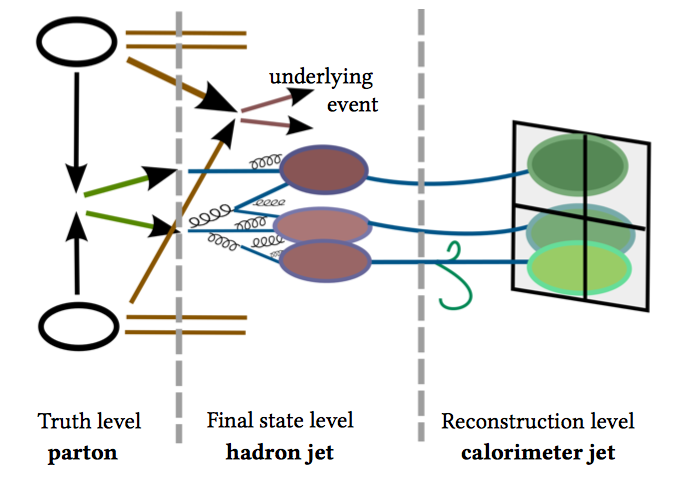
\includegraphics[scale=0.5]{images/sim_levels}
\caption{Illustration of the levels used in describing MC simulated high-energy collisions in the ATLAS detector. \cite{schnoor_thesis}}
\label{mc_levels}
\end{figure}
\subsection{The Hard Process}
In QED, calculations involve summing contributions from increasingly higher-order Feynman diagrams (i.e. perturbation theory), with the sum converging due to exponential dependence on the QED coupling constant $\alpha_{e}$  and the fact that $\alpha_{e} < 1$. This is not, in general, the case in QCD, where the running coupling constant $\alpha_{s}$ can exceed unity. This physically represents the confinement of quarks and gluons within hadrons. However, in special cases where, at sufficiently high energies and small distances, $\alpha_{s}$ decreases with the renormalisation scale $\mu_{R}$ until $\alpha_{s}$ becomes less than unity in what is called asymptotic freedom. The partons (quarks and gluons) can now be treated as free particles and perturbative QCD is applicable.

The \emph{factorisation therem} \cite{SM3} can be used in order to separate the sub-processes in a high energy scatter, into an infrared safe part (i.e. not dependent on the unknown, long-distance properties of QCD where perturbation theory breaks down) and a non-infrared safe part. For a scattering process $ab \longrightarrow n$, with initial hadronic particles $a$, $b$, and final state particles $n$, (illustrated in figure \ref{factorisation_theorem}), the factorisation theorem yields:
\begin{equation}
\sigma_{ab \rightarrow n} = \sum_{a,b}\int^{1}_{0}dx_{x}dx_{b}\int \underbrace{f_{a}^{h_{1}}(x_{a},\mu_{F})f_{b}^{h_{2}}(x_{b},\mu_{F})}_{\text{non-perturbative}}\underbrace{d\hat{\sigma}_{ab \rightarrow n}(\mu_{F},\mu_{R})}_{\text{perturbative}}.
\end{equation}
While the perturbation part can be calculated by treating the partons as free particles, the non-perturbative part must be inferred from the parton distribution functions (PDFs) $f_{i}^{h}(x_{i},\mu_{F})$ of the initial parton with respect to the original hadron $h$ with Bjorken $x_{i}$ and factorisation scale $\mu_{F}$. The PDF is the probability of finding a parton $i$, with Bjorken $x_{i}$ in a hadron $h$, at a energy scale $\mu_{F}$. The perturbative part constitutes the matrix element $| \mathcal{M}_{ab\rightarrow n} |^{2}$, so the cross-section be factorised as an integral over the final-state phase space $\Phi_{n}$:
\begin{equation}
\sigma_{ab \rightarrow n} = \sum_{a,b}\int^{1}_{0}dx_{x}dx_{b}\int d\Phi_{n} f_{a}^{h_{1}}(x_{a},\mu_{F})f_{b}^{h_{2}}(x_{b},\mu_{F}) \times \frac{1}{2\hat{s}}| \mathcal{M}_{ab\rightarrow n} |^{2} (\Phi _{n} ; \mu_{F},\mu_{R}).
\end{equation}
So the factorisation method allows for the cross-section to be calculated at the cost  of introducing a dependence on $\mu_{F}$. This is a very high dimensional integral and methods of MC integration are used for practicality.
\begin{figure}
\centering
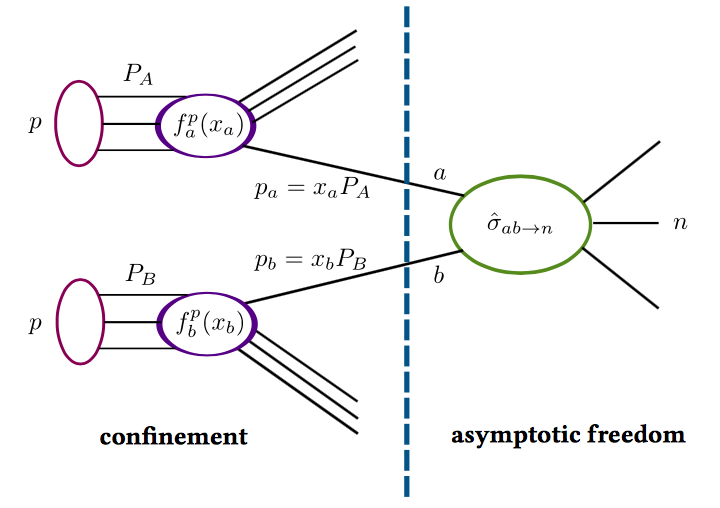
\includegraphics[scale=0.5]{images/factorisation_theorem.png}
\caption{An illustration of the factorisation theorem, showing how to the cross-section of a hadronic collision can be separated into a short distance part (where perturbative QCD is applicable) and a long distance part (where non-perturbative QCD must be used). \cite{schnoor_thesis}}
\label{factorisation_theorem}
\end{figure}
\subsection{Higher-Order Effects}
The final state particles from the evaluation of the fixed-order matrix-element are stable leptons and (non-observable) partons. Higher-order effects must be included to describe hadronisation, unstable particle decays, and the underlying event. These are each shown as components of a \textsc{Sherpa} simulated event in figure \ref{sherpa_event_sim}.
\begin{figure}
\centering
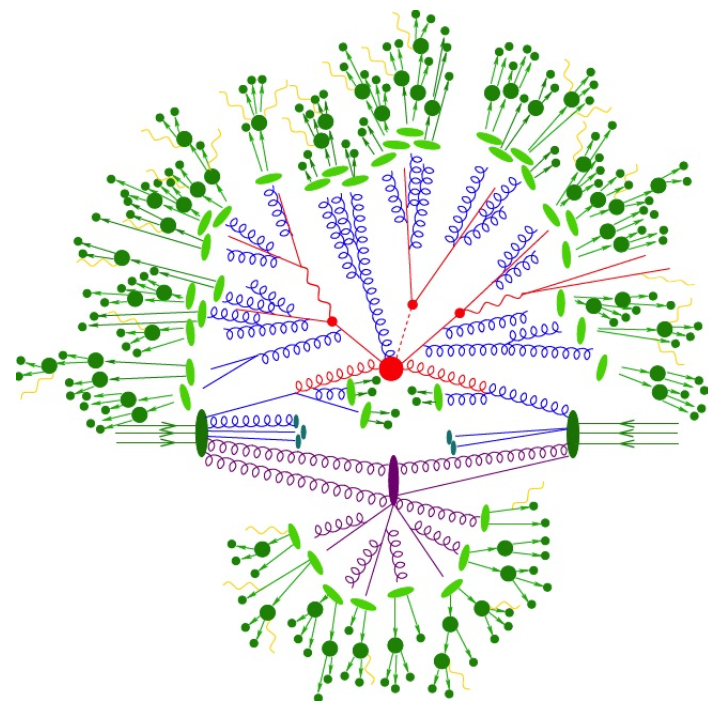
\includegraphics[scale=0.4]{images/sherpa_event_sim.png}
\caption{An illustration of a \textsc{Sherpa} generated event simulation. The hard interaction is shown in red, the partonic shower products in blue, the hadronised partons in green, hadronic decays in dark green, and the QED radiation in yellow. Note also the presence of the underlying event, coloured purple. \cite{SHERPA_image}}
\label{sherpa_event_sim}
\end{figure}
\subsubsection{Parton Shower}
Higher-order QCD effects can come from a parton showering and hadronisation algorithm. Parton showering is a complex process to simulate, as gluons carry colour and thus can trigger new additional QCD processes. Starting from the hard process (the process with the highest momentum scale), the parton shower simulation proceeds to successively lower momentum scales until the threshold of where perturbation theory is longer applicable is reached.
\subsubsection{Hadronisation}
The partons that result from the parton showering algorithm proceed to form colour-less bound states (hadrons), as described by the hadronisation algorithm. Unfortunately, hadronisation falls outside the region where perturbative QCD is applicable. As a result, hadronisation relies on QCD-inspired phenomenological models. Examples of such models are the \emph{string model} \cite{string_model}, which is based on linear confinement of partons, and the \emph{cluster model} \cite{cluster_model}, which is based on the pre-confinement of parton showers.
\subsubsection{Hadron and $\uptau$-Lepton Decays}
Many of the resulting hadrons that form, as described by the hadronisation algorithms, are unstable. These will decay before they can be directly measured by the detector. As a result, algorithms closely related to those used to model hadronisation, are used to simulate these hadronic decays. $\uptau$-leptons, produced in the original hard scattering process, also decay before they can be directly measured \cite{ATLAS}. Decay algorithms, that take into account spin effects, are used to simulate $\uptau$-lepton decays.
\subsubsection{QED Radiation}
QED radiation contributions are modeled in a similar way as the QCD parton shower but with electric charge in place of colour charge. Alternatively, the \emph{YFS formalism} \cite{YFS}, which is based on multipole evolution, can be used.
\subsubsection{Underlying Event}
Here the effects from the highly probable secondary interactions between proton remnants are considered. In the laboratory frame, the two colliding protons flatten into thin discs due to Lorentz contraction. The collision occurs when these two discs are approximately overlapping each other in space-time. This results in it being very likely that there will be other interactions aside from the hard process. These other processes are referred to as the underlying event. The hadrons that result contaminate the hard process. The underlying event is generally modeled in terms of additional interactions between the partons of the colliding protons.
\section{GEANT4: A Detector Simulator}
Simulating a detector's response to simulated data helps understand and optimise the way it will respond to actual physical processes and scenarios. The particles which result from a hard scatter will interact with the detector through random processes such as pair production, hadronic interactions with detector material, Coloumb scattering, or ionisation. Programming packages like GEANT4 (GEometry ANd Tracking) use MC techniques to simulate the passage of hard scatter products though detectors and gauge their response. To effectively simulate a detector, programming packages require descriptions of the detector's geometry and constituent material.

GEANT4 is a freely available toolkit used for simulating the passage of particles through matter. GEANT4 also provides a graphical representation of the experimental setup as well as the particles' trajectories. The experimental setup is described by the user in terms of geometrical volumes. The constituent materials of these volumes are also user-specified as this is required for GEANT4 to accurately model the detector's response to the traversing particles.

A basic summary of the working of GEANT4 is given here. Please see the documentation \cite{GEANT} for details. GEANT4 detector simulation is logically divided into three phases:
\begin{enumerate}
\item \textit{Initialisation}
\item \textit{Event Processing}
\item \textit{Termination}
\end{enumerate}
In \textit{Initialisation} GEANT4 prepares for particle transport. All geometrical information provided by the user is processed. Tables for energy loss and cross-section are computed and stored. Properties of the relevant particles and characteristics of the detector materials are also stored. In \textit{Event Processing}, each event is initialised, processed, and then cleaned from memory. Each particle is propagated through the setup and the detector's responses are simulated. These responses are stored along with the kinematics of the event. Once all events have been processed, GEANT4 proceeds to the final phase. The \textit{Termination} phase is user-controlled and commonly just computes and prints some statistical and technical information related to the preceding run.
\begin{figure}
\centering
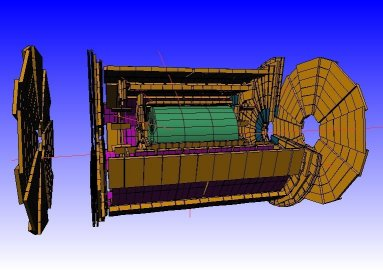
\includegraphics[scale=0.5]{images/geant_atlas.jpg}
\caption{GEANT4-created visualisation of the ATLAS detector. \cite{geant_atlas}}
\label{event_generator}
\end{figure}
\section{Simulation of the ATLAS Detector}
The actual application of the ATLAS detector simulation is done via the simulation chain, shown in figure \ref{sim_chain}. Initially, an MC generator generates events in \emph{HepMC} \cite{HEPMC} format. Next, events pass through the particle filter which applies some kinematic requirements. In the MCTruth (Gen) stage, the detector simulation uses generator level information, called MC truth, in order to simulate energy deposit signals. These simulated energy deposit are stored, along with their spatial coordinates, in ``Hits'' files. This forms part of the MC truth record. Similarly, in the simulation stage\footnote{This is the most computationally expensive step, taking several minutes per event.}, information of tracks and particle decays are also stored in the MC truth record. Simulated Data Objects (SDOs) are used to store associations between generator-level particles and simulated detector hits. Subsequently, the simulated analogue signals stored in the ``Hits'' files are converted into simulated digital signals that mimic those outputted from the detector Read-Out Drivers (RODs). At the same time, simulated pile-up contributions are added to the MC truth record. In the ultimate reconstruction step, the events are stored in bytestream format, to be subsequently converted into the Raw Data Objects (RDOs). It is important that they have the same format as actual data events recorded by the ATLAS detector, in order for the simulated data to be useful for calibration purposes and predicting the behaviour of real data.
\begin{figure}
\centering
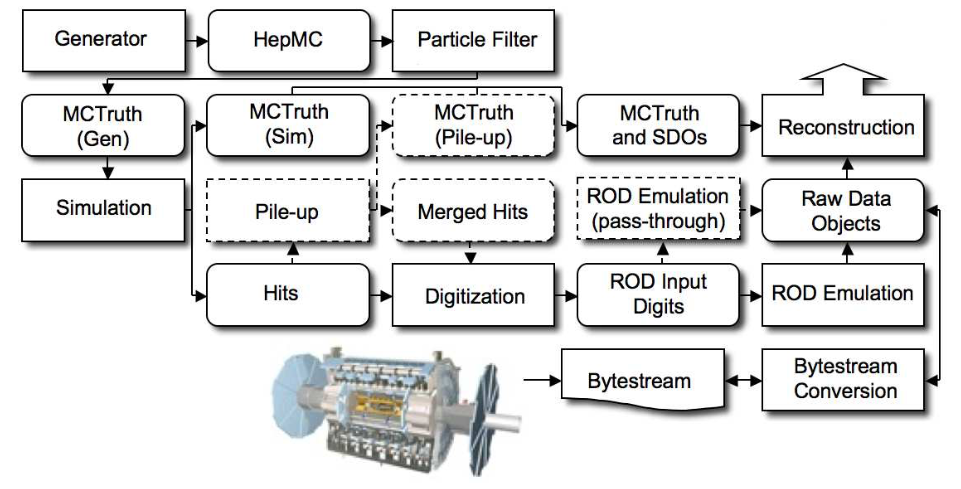
\includegraphics[scale=0.5]{images/atlas_sim_chain}
\caption{An illustration showing the ATLAS simulation chain. The boxes with the rounded corners represent persistent data objects, while those with sharp corners represent algorithms or applications. Optional algorithms have boxes made of dashed lines. \cite{ATLAS_sim}}
\label{sim_chain}
\end{figure} 
\chapter{Same-Sign W-boson Scattering Analysis}
\label{ssWW_analysis}
\section{Overview of Background Contributions}
Despite being distinctive, the experimental signature of same-sign W-boson scattering: $\ell^{\pm}\ell^{\pm} + jj + E_{T}^{miss}$, can still be faked by other Standard Model processes. These Standard Model background processes can be considered as falling into one two categories:
\begin{enumerate}
\item background processes where one or both leptons originate from jets or photons,
\item and all other background contributions, which can be sub-categorised as:
	\begin{enumerate}
	\item background processes that really do produce two same-sign leptons,
	\item and background processes that produce opposite-sign leptons where one of the leptons' charge is misidentified during reconstruction.
	\end{enumerate}
\end{enumerate}
Background contributions are also classified into prompt and non-prompt backgrounds. Leptons coming from a W-boson are said to be prompt (making up the prompt background), while those coming from the decay of a hadron or a $\uptau$-lepton are said to be non-prompt (making up the non-prompt background).

Expanding upon the above classifications, same-sign W-boson scattering backgrounds can be specifically associated with three sources:
\begin{itemize}
\item Backgrounds resulting from jet-faked leptons are examples of category 1. These are processes in which one or two jets are misreconstructed as leptons or give rise to non-prompt leptons. Lepton quality and isolation requirements, as well as the $b$-jet veto and $E_{T}^{miss}$ requirements are used to suppress such processes, including: $W$ + $jets$, $t\bar{t}$, single top, or QCD multijet processes. Additionally, $W\gamma$ + $jets$ processes where the photon is misreconstructed as an electron, are also an example from category 1. Lepton quality, isolation requirements, and a veto on any events with a third lepton are used for suppression.
\item Processes where three or four leptons are produced, but only two leptons are reconstructed, are examples of sub-category 2.a. This can happen in the case of $WZ$ + $jets$ where the lepton from the W decay and the same-sign lepton from the Z decay pass all selection requirements while the remaining lepton is not reconstructed.
\item Background contributions resulting from charge misidentification (mis-ID) are examples of sub-category 2.b. These are opposite-sign processes where the sign of one lepton is misreconstructed. This can happen due to bremsstrahlung, where an lepton radiates a high energy photon which then pair produces with one of the resulting leptons reconstructed. The power radiated is proportional to $m^{-4}$ for when acceleration is perpendicular to the direction of motion, and $m^{-6}$ for when acceleration is parrallel to the direction of motion \cite{brem}; where $m$ is the particle's mass. In reality, any accelerating particle will have components of its acceleration both perpendicular and parrallel to its motion. However, even for motion that is purely perpendicular to the acceleration, as is the case in circular motion, heavier particles will radiate less than lighter particles (since the power radiated is still proportional to $m^{-4}$). Due to this mass dependence, electrons tend to radiate more energy than the heavier muons. The charge misidentification rate is hence higher for electrons than muons. Processes that contribute to the charge misidentification background include: $t\bar{t}$ \footnote{$t\bar{t}$ processes contribute to both of our two main categories. Semi-leptonic $t\bar{t}$ decays contribute to the non-prompt background (part of category 1), while in other cases, where the top quarks decay fully leptonically, they contribute to they contribute to the prompt background (part of the second category 2.). The two prompt leptons produced in the fully leptonic decay will be opposite-sign rather than same-sign, so this background comes from charge misidentification.}, $W^{\pm}W^{\pm}$ + $jets$, and $Z/\gamma^{*}$ + $jets$ $\longrightarrow \ell^{\pm}\ell^{\pm}$ + $jets$. A veto on events in which a $b$-jet is tagged ($b$-jet veto) is used to help suppress contributions from $t\bar{t}$, while a Z-mass veto is used to suppress $Z/\gamma^{*} \longrightarrow e^{+}e^{-}$, in the $ee$ channel.
\end{itemize}
\section{Object Selection}
\label{object_selection}
Physics objects in the analysis of same-sign W-boson scattering events are required to pass selection requirements in order to help suppress backgrounds coming from other Standard Model processes. This section describes the criteria for objects relevant to same-sign W-boson scattering analysis, i.e. electrons, muons, jets, and overlap removal.
\subsection{Triggers}
The high-level trigger is configured to trigger on electrons that have $p_{T} \geq 24$ GeV and pass the medium electron quality requirements, or alternatively, $p_{T} > 120$ GeV and pass the loose muon quality requirements. Muons trigger on $p_{T} > 50$ GeV, or on $p_{T} > 20$ GeV provided the muon also passes a loose isolation requirement (see \cite{trigger} for details).
\subsection{Muons}
Kinematic cuts are employed in order to reduce the contribution of muons from pile-up collisions and the multijet background. A given muon candidate is required to have an associated track in the inner detector that originates from the primary vertex. In practice this is done by requiring that the muon's flight path intersects the beam axis (z-axis) within 0.5 mm of the primary vertex and that the $d_{0}$ significance is less than 3. Furthermore, the muon is required to have a $p_{T} > 25$ GeV, and fall within a geometrical acceptance of $| \eta | < 2.5$. The $ | \eta | $ requirement corresponds to the total coverage of the precision-tracking (pixel and SCT) detectors. A muon candidate must also pass the default identification requirement, which only allows stand-alone or combined tracks (see section \ref{muon_reco}). These requirements are summarised in table \ref{tight_muon}.

\begin{table}[h]
	\centering{
	\begin{tabular}{c}
	Muon Selection \\ \hline \hline
	Identification: stand-alone or combined tracks \\ \hline
	Isolation: \textit{Gradient} \\ \hline
	Kinematic Acceptance: $p_{T} > 27$ GeV \\ \hline
	Geometrical Acceptance: $| \eta | < 2.5$ \\ \hline
	Longitudinal Impact parameter requirement: $| z_{0} \times \sin \theta | < 0.5$ mm \\
	Transverse Impact parameter requirement: $\frac{d_{0}}{\sigma_{d_{0}}} < 3$ \\ \hline \hline
	\end{tabular}}
	\caption{Signal muon definition}
	\label{tight_muon}
\end{table}

In the implementation of the third lepton veto (see section \ref{event_selection}), a looser selection criteria is applied to candidate veto muons; see table \ref{loose_muon}.

\begin{table}[h]
	\centering{
	\begin{tabular}{c}
	Muon Selection \\ \hline \hline
	Identification: stand-alone or combined tracks \\ \hline
	Isolation: \textit{LooseGradient} \\ \hline
	Kinematic Acceptance: $p_{T} > 10$ GeV \\ \hline
	Geometrical Acceptance: $| \eta | < 2.5$ \\ \hline
	Longitudinal Impact parameter requirement: $| z_{0} \times \sin \theta | < 0.5$ mm \\
	Transverse Impact parameter requirement: $\frac{d_{0}}{\sigma_{d_{0}}} < 3$ \\ \hline \hline
	\end{tabular}}
	\caption{Veto muon definition}
	\label{loose_muon}
\end{table}

\subsection{Electrons}
Electrons are reconstructed using energy deposits in the calorimeter together with the associated matched tracks in the inner-detector. Candidates are required to pass the tight cut definition selection criteria, described in section \ref{electron_reco}, and encompasses cuts based on shower shape, track quality, detection of transition radiation, and track-to-calorimeter-cluster matching (see tight cuts selection in section \ref{electron_reco}). Additional requirements include $p_{T} > 27$ GeV, and a geometrical acceptance of $| \eta | < 1.37$. Note that the $ | \eta | $ requirement restricts electron reconstruction to the barrel region of the electromagnetic calorimeter. These requirements are summarised in table \ref{tight_electron}.

\begin{table}[h]
	\centering{
	\begin{tabular}{c}
	Electron Selection \\ \hline \hline
	Identification: tight cut selection \\ \hline
	Isolation: \textit{Gradient} \\ \hline
	Kinematic Acceptance: $p_{T} > 27$ GeV \\ \hline
	Geometrical Acceptance: $| \eta | < 1.37$ \\ \hline
	Longitudinal Impact parameter requirement: $| z_{0} \times \sin \theta | < 0.5$ mm \\
	Transverse Impact parameter requirement: $\frac{d_{0}}{\sigma_{d_{0}}} < 5$ \\ \hline \hline
	\end{tabular}}
	\caption{Signal electron definition}
	\label{tight_electron}
\end{table}

\begin{table}[h]
	\centering{
	\begin{tabular}{c}
	Electron Selection \\ \hline \hline
	Identification: medium cut selection\\ \hline
	Isolation: \textit{LooseGradient} \\ \hline
	Kinematic Acceptance: $E_{T} > 10$ GeV \\ \hline
	Geometrical Acceptance: $| \eta | < 2.47$, outside crack region $1.37 \geq | \eta | \geq 1.52$ \\ \hline
	Longitudinal Impact parameter requirement: $| z_{0} \times \sin \theta | < 0.5$ mm \\
	Transverse Impact parameter requirement: $\frac{d_{0}}{\sigma_{d_{0}}} < 5$ \\ \hline \hline
	\end{tabular}}
	\caption{Veto electron definition}
	\label{loose_electron}
\end{table}

Like muons, candidate veto electrons (for the third lepton veto) are subjected to a looser a set of requirements. They are only require to pass the medium selection cuts, given in section \ref{electron_reco}. See table \ref{loose_electron} for summary.
\subsection{Jets}
Jets are reconstructed using the \emph{anti-$k_{t}$} algorithm from topological calorimeter clusters. The jets are then calibrated from the electromagnetic energy scale to the hadronic energy scale using a correction factor \cite{JetCorrection}, dependent on $E_{T}$ and $\eta$, from Monte Carlo simulations. A same-sign W-boson scattering event results in two forward jets. Therefore event candidates must have at least two jets with $p_{T} > 30$ GeV and $| \eta | < 4.5$. The two jets with the highest $p_{T}$ are designated the tagging jets.
\subsection{Overlap Removal}
It is possible for a single physics object to be reconstructed multiple tines and, conversely, for two distinct objects may be sufficiently spatially overlap that they are misreconstructed as a single object. The overlap removal procedure is intended to reduce such instances. The overlap procedure used in this analysis is that followed by the Analysis Harmonisation Group \cite{OLR}, and examines and removes objects in a pre-defined order, described as follows:
\begin{enumerate}
\item electron/jet: If the calorimeter cluster associated with an electron, overlaps with that of a jet within $\Delta R =0.3$, both objects are removed.
\item electron/muon: A muon may be misreconstructed as an electron if it's associated track in the I.D. is matched to an electromagnetic cluster resulting from bremsstrahlung. Hence, if a reconstructed electron lies within $ \Delta R =0.1$ of a reconstructed muon, the electron is removed.
\item As previously mentioned, muons coming from the decay of a hadron are part of the non-prompt background. Hence, any muon found to be within $\Delta R =0.3$ of a jet results in the whole event being vetoed.
\end{enumerate}
\section{Event Selection}
\label{event_selection}
In addition to applying a selection criteria to same-sign W-boson scattering candidate objects in order to reduce backgrounds from other Standard Model processes, additional requirements are imposed on candidate events in order to further suppress undesirable background contributions. To this end a series of cuts are applied to candidate events:
\begin{enumerate}
\item any event in which the primary vertex has less than three associated tracks is vetoed,
\item exactly two leptons with $m_{\ell \ell '} > 20$ GeV,
\item any events with additional leptons are excluded (third lepton veto),
\item $q_{\ell _{1}} \times q_{\ell _{2}} > 0$ (same-sign),
\item $|m_{ee} - m_{Z}| > 15$ GeV ($ee$ channel only),
\item $E_{T}^{miss} \geq 10$ GeV,
\item a minimum of two jets with $p_{T} > 30$ GeV and $|\eta | < 4.5$,
\item $b$-jet veto using the ATLAS Run 2 multivariate b-tagger with the $70\%$ working point,
\item $m_{jj} \geq 500$ GeV,
\item $| \Delta y_{jj} | > 2.3$.
\end{enumerate}

Cut 1 involves cleaning cuts applied to events that pass the \textsc{HLT}, including: vetoing incomplete events, requiring at least one vertex with at least three associated tracks with $p_{T} > 0.5$ GeV, cleaning of jets\footnote{Jet cleaning is the process of applying some selection criteria to remove jets that may be fake (sources of fake jets include LHC beam conditions, known hardware malfunctions, and coming from cosmic ray showers), or are likely to be mismeasured \cite{jet_cleaning}.}, and \textsc{GRL} (Good Runs List\footnote{A luminousity block is a time period of approximately two minutes associated with data taking. The Good Runs List is used to select only ``good'' luminousity blocks. ``Bad'' luminousity blocks are those that do not contain viable data for a variety of regions, e.g. sub-detectors were switched off, the LHC beam was not stable, or the magnets were off or ramping.}) selection.

Cuts 2 to 4 correspond to selecting events with exactly two same-sign leptons. The invariant mass requirement is used to reduce the uncertainty in modelling low mass Drell-Yan\footnote{A Drell-Yan process is a process in which a quark and an antiquark (from distinct hadrons) annihilate, creating a virtual $\gamma/Z$ which then decays to a pair of opposite-sign leptons.} processes.

Cut 5 is a Z-mass veto cut intended to reduce the Drell-Yan background $Z \longrightarrow ee$, where one of the lepton's charges is misreconstructed.

The pair of escaping neutrinos carry away some transverse energy. Hence cut 6 cuts out events that lack sufficient $E_{T}^{miss}$ to be from a same-sign W-boson scattering event.

Cut 8, a $b$-jet veto, is used to reduce background contributions coming from top processes.

The last two cuts deal with the forward tagging jets. They are required to have an invariant mass of at least 500 GeV (cut 9), and be separated in rapidity by at least 2.4 (cut 10 ).
\section{Fake Lepton Background}
\label{intro_to_flb}
Non-prompt leptons, which result from the decay of a hadron together with jets misreconstructed as leptons, are referred to as jet-faked leptons. Processes where a prompt lepton is reconstructed along with a jet-faked lepton contribute to background in events selected for measurement of same-sign W-boson scattering. This background is subsequently referred to as the jet-faked lepton background or simply \emph{fake lepton background}. Dominant contributions to the fake lepton background come from $W$ + $jets$, $t\bar{t} \longrightarrow WbWb \longrightarrow \ell \nu bb qq$, and single top processes. In each case a W-boson decays leptonically with the second lepton being jet-faked. The degree to which leptons are isolated (see section \ref{isolation_section}) can be used to reduce the fake lepton background.

Some common processes which contribute to the \emph{fake lepton background} involve the decay of a top quark to a bottom quark by emission of a $W^{+}$, e.g. a semi-leptonic $t\bar{t}$ process (see figure \ref{semi-leptonic_ttbar}). Top-quarks overwhelmingly decay to bottom-quarks through emission of a W-boson \cite{PDG}. Thus implementing a veto on any event that is found to contain a b-jet can help suppress the fake lepton background.

\begin{figure}
\centering{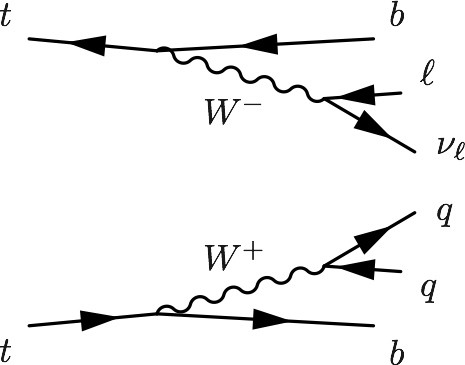
\includegraphics[scale=0.5]{images/semi-leptonic_ttbar.png}}
\caption{Feynman diagram for a semi-leptonic $t\bar{t}$ decay. In same-sign W-boson scattering such processes can contribute to the fake lepton background if one of the resulting jet is misreconstructed as a lepton of the same-sign as the other reconstructed lepton.}
\label{semi-leptonic_ttbar}
\end{figure}
\chapter{Suppressing the Fake Lepton Background}
For the simulated data used in this chapter, the \textsc{Sherpa} event generator was used for the signal $W+W+jj$ process, as well as the background processes: $Z+jets$, $ZZ$, $W+\gamma$, $W+jets$, and $WZ$. All diboson samples used the CT10 parton distribution function set \cite{CT10}. The single top and $t\bar{t}$ processes were generated by \textsc{PowHeg-Box}, and \textsc{Madgraph} was used for the $t\bar{t}+V$ process with showering algorithm handled by \textsc{Pythia}. $\uptau$-lepton decays were handled with the \textsc{Sherpa} parton showering algorithm. The output from each event generator was inputted into a GEANT4-based framework for detector simulation. The resulting MC samples were then post-processed, calibrated, and had some loose selection requirements applied to the physics objects. Unless otherwise stated, the object and event selections, as described in sections \ref{object_selection} and \ref{event_selection} respectively, were applied. The simulated data was normalised to an integrated luminosity of $28.0$fb$^{-1}$. The integrated luminosity was assumed was in line with the amount of run 2 data available for analysis when the simulated data was produced.
\section{Statistical Significance in Particle Physics}
In an experimental analysis, it is desirable to have as large an excess of signal events $s$ over expected background events $b$ as possible. This is commonly called the signal-to-background ratio $s/b$. In particle physics, Monte Carlo simulations are often used in order to determine an expected signal-to-background ratio, to more easily identify excesses in experimental data. Experimental analysis cuts are often optimised to maximise the signal-to-background ratio for this reason. However, in cases where the signal-to-background ratio is low but the number of total events is sufficiently large, signal excesses may still be identified and analysed regardless. Essentially being discrete counting experiments, statistical fluctuations in particle and nuclear physics experiments are Poissonian; i.e. $\sigma = \sqrt{N}$, where $N$ is the total number of event. The statistical significance is the number of standard deviations dividing a signal excess, thus since $N= s+b$, the significance in particle physics is given by:
$$ \frac{excess}{\sigma} = \frac{s}{\sqrt{s+b}}.$$ 
In practice, it is preferable to optimise based on the significance $s/\sqrt{s+b}$, rather than $s/b$, in instances where there is only a small signal excess relative to the total number of events.
\section{Optimising the $b$-jet Veto}
As mentioned in section \ref{intro_to_flb}, a veto on events found to contain a $b$-jet is used in the analysis of same-sign W-boson scattering events. This is used to suppress the non-prompt background, as the dominant contribution (see in table \ref{non-prompt_table}) comes from $t\bar{t}$ events where the top decays semi-leptonically, through emission of a $b$-quark. The means by which $b$-jets are identified in ATLAS is described in sub-section \ref{mva}. The multivariate $b$-tagger has four working points (see table \ref{b-tagger_working_points}), each with a corresponding efficiency. Implementing the $b$-tagger with the 85$\%$ efficiency means that the tagger will identify approximately 85$\%$ of all $b$-jets in a given event. The higher the efficiency of the $b$-tagger, the more jets will be tagged as being $b$-flavoured. Conversely, the purity (the percentage of tagged jets having $b$-flavour) decreases with efficiency. 
\begin{table}
	\centering{\begin{tabular}{|c|c|c|c|}
	\hline
	 & \multicolumn{3}{|c|}{non-prompt background} \\ \hline
	\textbf{$b$-jet veto} & $W$ + jets & $t\bar{t}$ & single top \\ \hline
	before & $79.54 \pm 38.19$ & $442.27 \pm 10.26$ & $37.43 \pm 2.12$ \\ \hline
	after & $77.15 \pm 38.17$ & $89.32 \pm 4.28$ & $12.71 \pm 1.22$ \\ \hline
	\end{tabular}}
	\caption{Number of events, across all channels, originating from each of the main contributors to the non-prompt background, before and after the $b$-jet veto is implemented. The multivariate $b$-tagger 70$\%$ efficiency working point was used. Note that $t\bar{t}$ events are are the dominant contributor. The cuts implemented before the veto are listed in chapter \ref{ssWW_analysis}. Errors displayed are purely statistical.}
	\label{non-prompt_table}
\end{table}

In order to determine the optimal multivariate $b$-tagger working point to use in the analysis of same-sign W-boson scattering, the significance at each working point is calculated and the working point at which the maximum significance occurs is designated the optimal working point. Recall that the other primary tools for reducing the fake lepton background, are the isolation selection requirements that are imposed on the lepton candidates. The multivariate $b$-tagger working point is optimised with all of the object selection criteria, including having the lepton candidates pass the \textit{Gradient} isolation selection requirement. It is also optimised for an alternate case, for when the lepton candidates are not required to pass any isolation selection requirements, as a control. This is not expected to perform as well as the \textit{Gradient} isolation selection requirement case as its lack makes it more likely that jet-faked leptons will pass the lepton candidate definitions. The working points are optimised individually for each analysis channel ($ee$, $e\mu +\mu e$, and $\mu\mu$) mentioned in section \ref{ssWW_intro}, as well as for the total across all channels. The ATLAS same-sign W-boson analysis is currently using the 85$\%$ efficiency working point.

Figure \ref{optimal_b-tagging_working_point_wGrad} and table \ref{b-tagging_working_point_wGrad_numbers} show the results of the optimisation study for the \textit{Gradient} isolation selection requirement case. Note that the maximum for the total over all channels occurs at the $70\%$ working point. For the $ee$, $e \mu + \mu e$, and $\mu\mu$ channels, the maximum significances occur at the $70\%$, $60\%$, and $70\%$ working points respectively. Also note that, aside from using the 0$\%$ efficiency (i.e. not having a $b$-jet veto), the currently used 85$\%$ efficiency working point performs the worst compared to all others. However, also note that the significances for all the non-zero efficiencies overlap within uncertainty. This is true per channel as well for the total.

On the other hand, figure \ref{optimal_b-tagging_working_point_noIso} and table \ref{b-tagging_working_point_noIso_numbers}, show the results of the alternate case for where the lepton candidates have no isolation selection requirements. Note that the maximum for the total over all channels occurs at the $70\%$ working point. For the $ee$, $e \mu + \mu e$, and $\mu\mu$ channels, the maximum significances occur at the $70\%$, $77\%$, and $70\%$ working points respectively. As with the first plot, the significances per channel as well as the total overlap within statistical uncertainty.

Comparing the two figures: note that the best approximation 3.38 of the maximum significance for the total across all channels, is achieved at the 70$\%$ efficiency, which is lower than that of the worst performing efficiency 0$\%$ working point for the first (requiring \textit{Gradient} isolation selection on lepton candidates) case, which has a best approximation to the significance of $3.46$. The values do overlap however, when the statistical uncertainty is taken into account. Like the first case, the 85$\%$ efficiency working point performs the worst when compared to the other non-zero efficiency working points.

While the two cases do not agree on the optimal working point for the $e\mu +\mu e$ channel, they are both in agreement that the $70\%$ multivariate working point performs best when considering the best approximations to the significance. These results considering the best approximations to the significance alone suggest moving from the currently used 85$\%$ efficiency working point to the 70$\%$ efficiency working point. This would increase the significance by approximately 5$\%$. The reason for this is that while the 85$\%$ efficiency working point tags more events containing a $b$-jet (and hence vetoes more background events), it also vetoes more signal events. This can be seen from the numbers in table \ref{b-tagging_working_point_wGrad_numbers}, where in the 85$\%$ efficiency, the background decreases by 12$\%$ compared to the 70$\%$ efficiency. However, the signal also decreases by 11$\%$, and due to the significance quantity $s/\sqrt{s+b}$ being more sensitive to decreases in signal events, this has the effect of resulting in an overall lower significance for the 85$\%$ efficiency working point when compared to the 70$\%$ working point. This study suggests then that the optimal $b$-tagger efficiency is the 70$\%$ working point. It should be stressed however, that this is a weak assertion given that, when the uncertainties are taken into account, the differences in the significances between each efficiency working point are not statistically significant, i.e. it could be a statistical fluctuation. Further studies, using larger sample sizes are necessary to determine whether to move to efficiency working point from 85$\%$ to 70$\%$ is warranted.

The studies also suggest that the \textit{Gradient} isolation selection has the effect of increasing the significance across all channels and efficiency working points. This was not, however, unexpected.
\begin{table}
	\resizebox{\textwidth}{!}{\centering{\begin{tabular}{|l|c|c|c|c|c|}
	\hline
	Working Point & $0\%$ & $60\%$ & $70\%$ & $77\%$ & $85\%$ \\ \hline \hline
	$ee$ bkg. & $30.83 \pm 4.02$ & $19.36 \pm 3.67$ & $18.26 \pm 3.64$ & $17.38 \pm 3.62$ & $16.30 \pm 3.59$ \\ \hline
	$e\mu + \mu e$ bkg. & $46.16 \pm 3.02$ & $29.72 \pm 2.49$ & $28.57 \pm 2.47$ & $26.61 \pm 2.38$ & $26.61 \pm 2.38$ \\ \hline
	$\mu\mu$ bkg. & $19.77 \pm 1.54$ & $16.20 \pm 1.48$ & $15.06 \pm 1.39$ & $14.32 \pm 1.36$ & $12.56 \pm 1.27$ \\ \hline
	total bkg. & $96.76 \pm 5.26$ & $67.07 \pm 4.70$ & $63.06 \pm 4.62$ & $60.27 \pm 4.59$ & $55.47 \pm 4.49$ \\ \hline
	$ee$ sig. & $5.82 \pm 0.13$ & $5.71 \pm 0.13$ & $5.59 \pm 0.12$ & $5.43 \pm 0.12$ & $4.99 \pm 0.12$ \\ \hline
	$e \mu + \mu e$ sig. & $20.71 \pm 0.24$ & $20.26 \pm 0.24$ & $ 19.86 \pm 0.23$ & $19.25 \pm 0.23$ & $17.67 \pm 0.22$ \\ \hline
	$\mu\mu$ sig. & $14.01 \pm 0.20$ & $ 13.74 \pm 0.19$ & $13.48 \pm 0.19$ & $13.08 \pm 0.19$ & $11.98 \pm 0.18$ \\ \hline
	total sig. & $40.54 \pm 0.34$ & $39.71 \pm 0.33$ & $38.93 \pm 0.32$ & $37.76 \pm 0.32$ & $34.64 \pm 0.31$ \\ \hline
	total $s/\sqrt{s+b}$ & $3.46 \pm 0.07$ & $3.843 \pm 0.09$ & $3.86 \pm 0.09$ & $3.81 \pm 0.09$ & $3.65 \pm 0.10$ \\ \hline
	\end{tabular}}}
\caption{Number of signal and background events by channel and multivariate $b$-tagger efficiency working point. The total significance is given in the bottom row for each efficiency working point. The lepton candidates must pass the \textit{Gradient} isolation selection requirement. Errors displayed are purely statistical}
\label{b-tagging_working_point_wGrad_numbers}
\end{table}
\begin{table}
	\resizebox{\textwidth}{!}{\centering{\begin{tabular}{|l|c|c|c|c|c|}
	\hline
	Working Point & $0\%$ & $60\%$ & $70\%$ & $77\%$ & $85\%$ \\ \hline \hline
	$ee$ bkg. & $41.62 \pm 4.32$ & $26.18 \pm 3.88$ & $24.45 \pm 3.85$ & $22.99 \pm 3.81$ & $21.26 \pm 3.78$ \\ \hline
	$e\mu + \mu e$ bkg. & $82.76 \pm 4.21$ & $55.16 \pm 3.50$ & $51.29 \pm 3.42$ & $47.64 \pm 3.32$ & $43.11 \pm 3.19$ \\ \hline
	$\mu\mu$ bkg. & $50.45 \pm 9.22$ & $39.17 \pm 9.11$ & $36.95 \pm 9.08$ & $35.26 \pm 9.06$ & $31.99 \pm 9.04$ \\ \hline
	total bkg. & $174.83 \pm 11.02$ & $120.51 \pm 10.50$ & $112.69 \pm 10.44$ & $105.89 \pm 10.37$ & $96.36 \pm 10.30$ \\ \hline
	$ee$ sig. & $6.22 \pm 0.13$ & $6.09 \pm 0.13$ & $5.96 \pm 0.13$ & $5.78 \pm 0.13$ & $5.32 \pm 0.12$ \\ \hline
	$e \mu + \mu e$ sig. & $22.41 \pm 0.25$ & $21.91 \pm 0.25$ & $ 21.46 \pm 0.24$ & $20.81 \pm 0.24$ & $19.08 \pm 0.23$ \\ \hline
	$\mu\mu$ sig. & $15.20 \pm 0.20$ & $14.91 \pm 0.20$ & $14.63 \pm 0.20$ & $14.19 \pm 0.20$ & $13.02 \pm 0.19$ \\ \hline
	total sig. & $43.83 \pm 0.35$ & $42.91 \pm 0.34$ & $42.05 \pm 0.34$ & $40.78 \pm 0.34$ & $37.42 \pm 0.32$ \\ \hline
	total $s/\sqrt{s+b}$ & $2.96 \pm 0.08$ & $3.36 \pm 0.11$ & $3.38 \pm 0.12$ & $3.37 \pm 0.12$ & $3.24 \pm 0.13$ \\ \hline
	\end{tabular}}}
\caption{Number of signal and background events by channel and multivariate $b$-tagger efficiency working point. The total significance is given in the bottom row for each efficiency working point. The lepton candidates are not required to pass any isolation selection criteria. Errors displayed are purely statistical.}
\label{b-tagging_working_point_noIso_numbers}
\end{table}
\begin{figure}
\centering{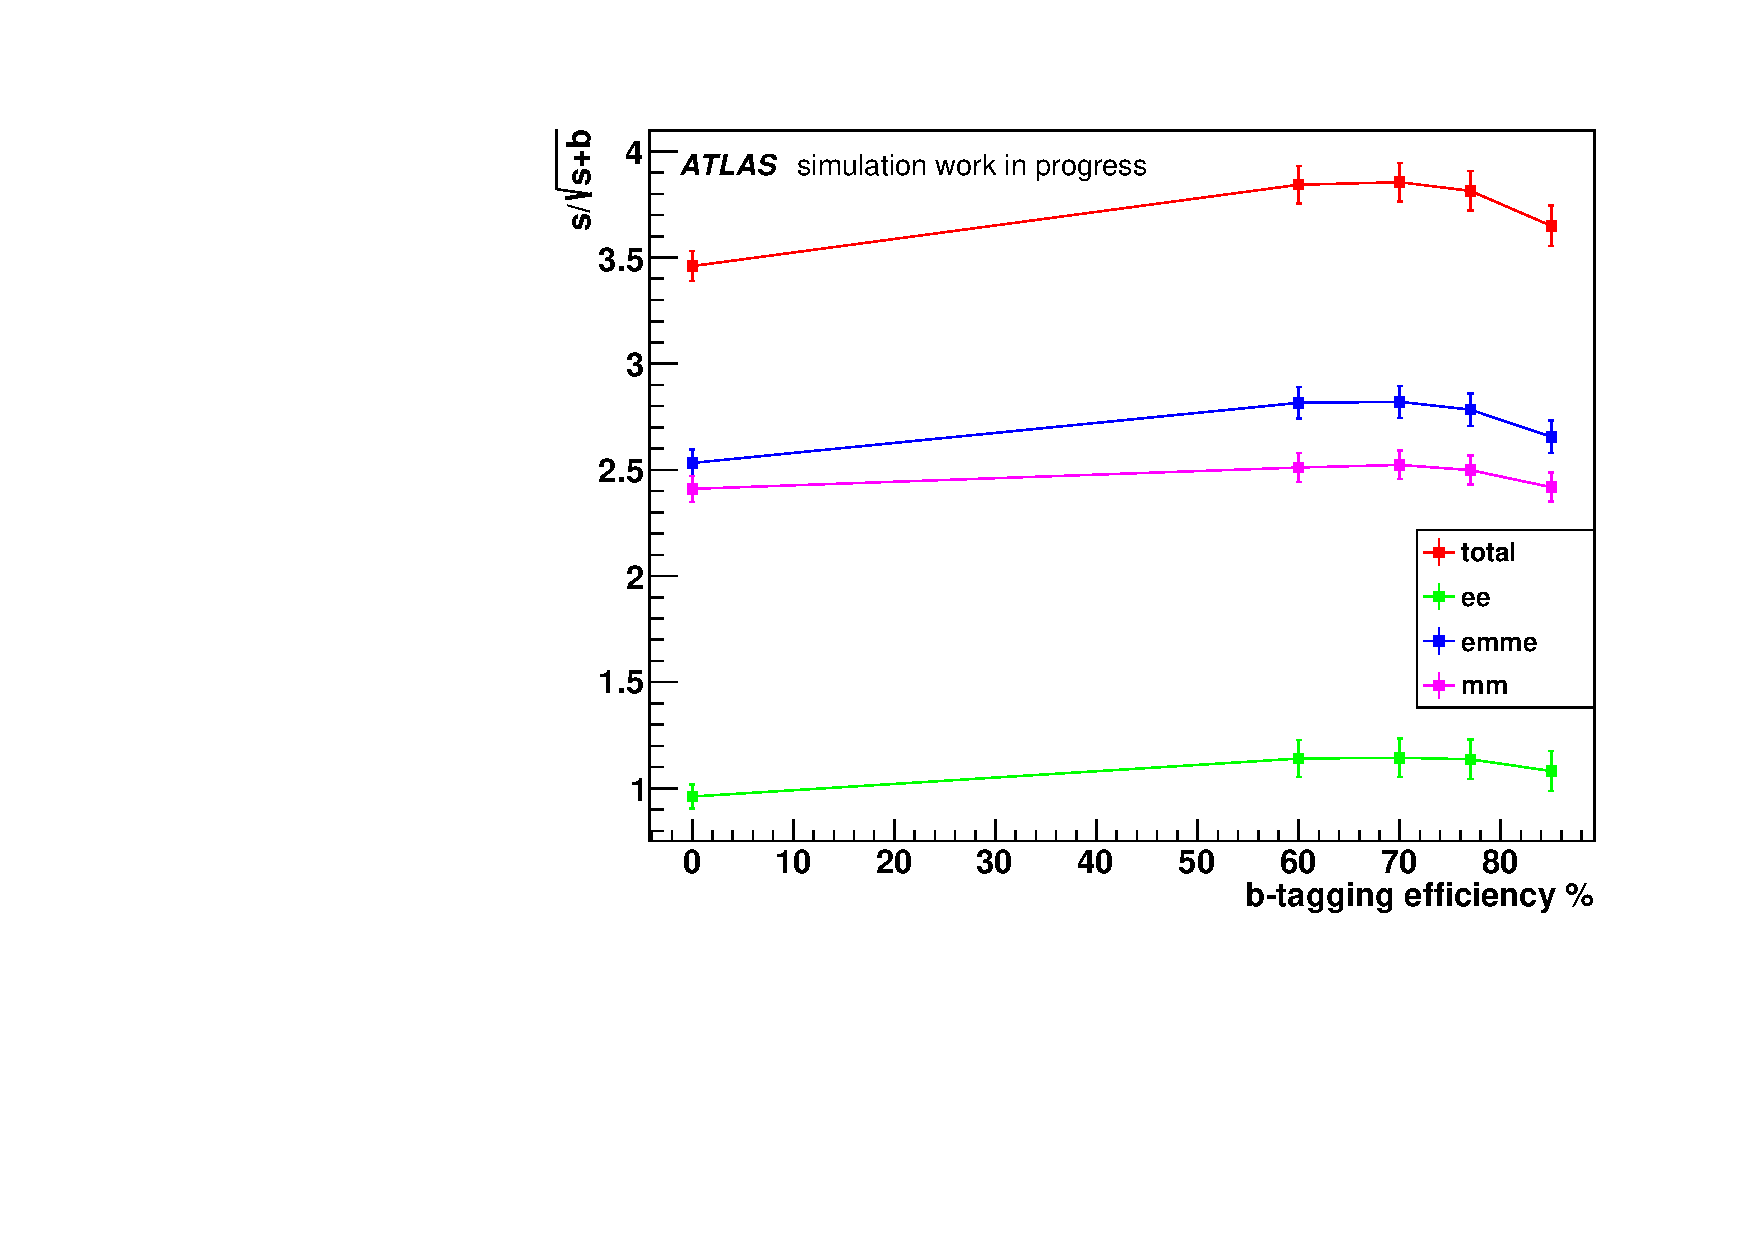
\includegraphics[width=1.\textwidth]{images/chapter7/Grad_stbr_btag_better.pdf}}
\caption{The significance at each multivariate $b$-tagger working point as well as the significance at $0\%$ (which corresponds to not using a $b$-jet veto at all). Lepton candidates were required to pass the \textit{Gradient} isolation requirement.}
\label{optimal_b-tagging_working_point_wGrad}
\end{figure}
\begin{figure}
\centering{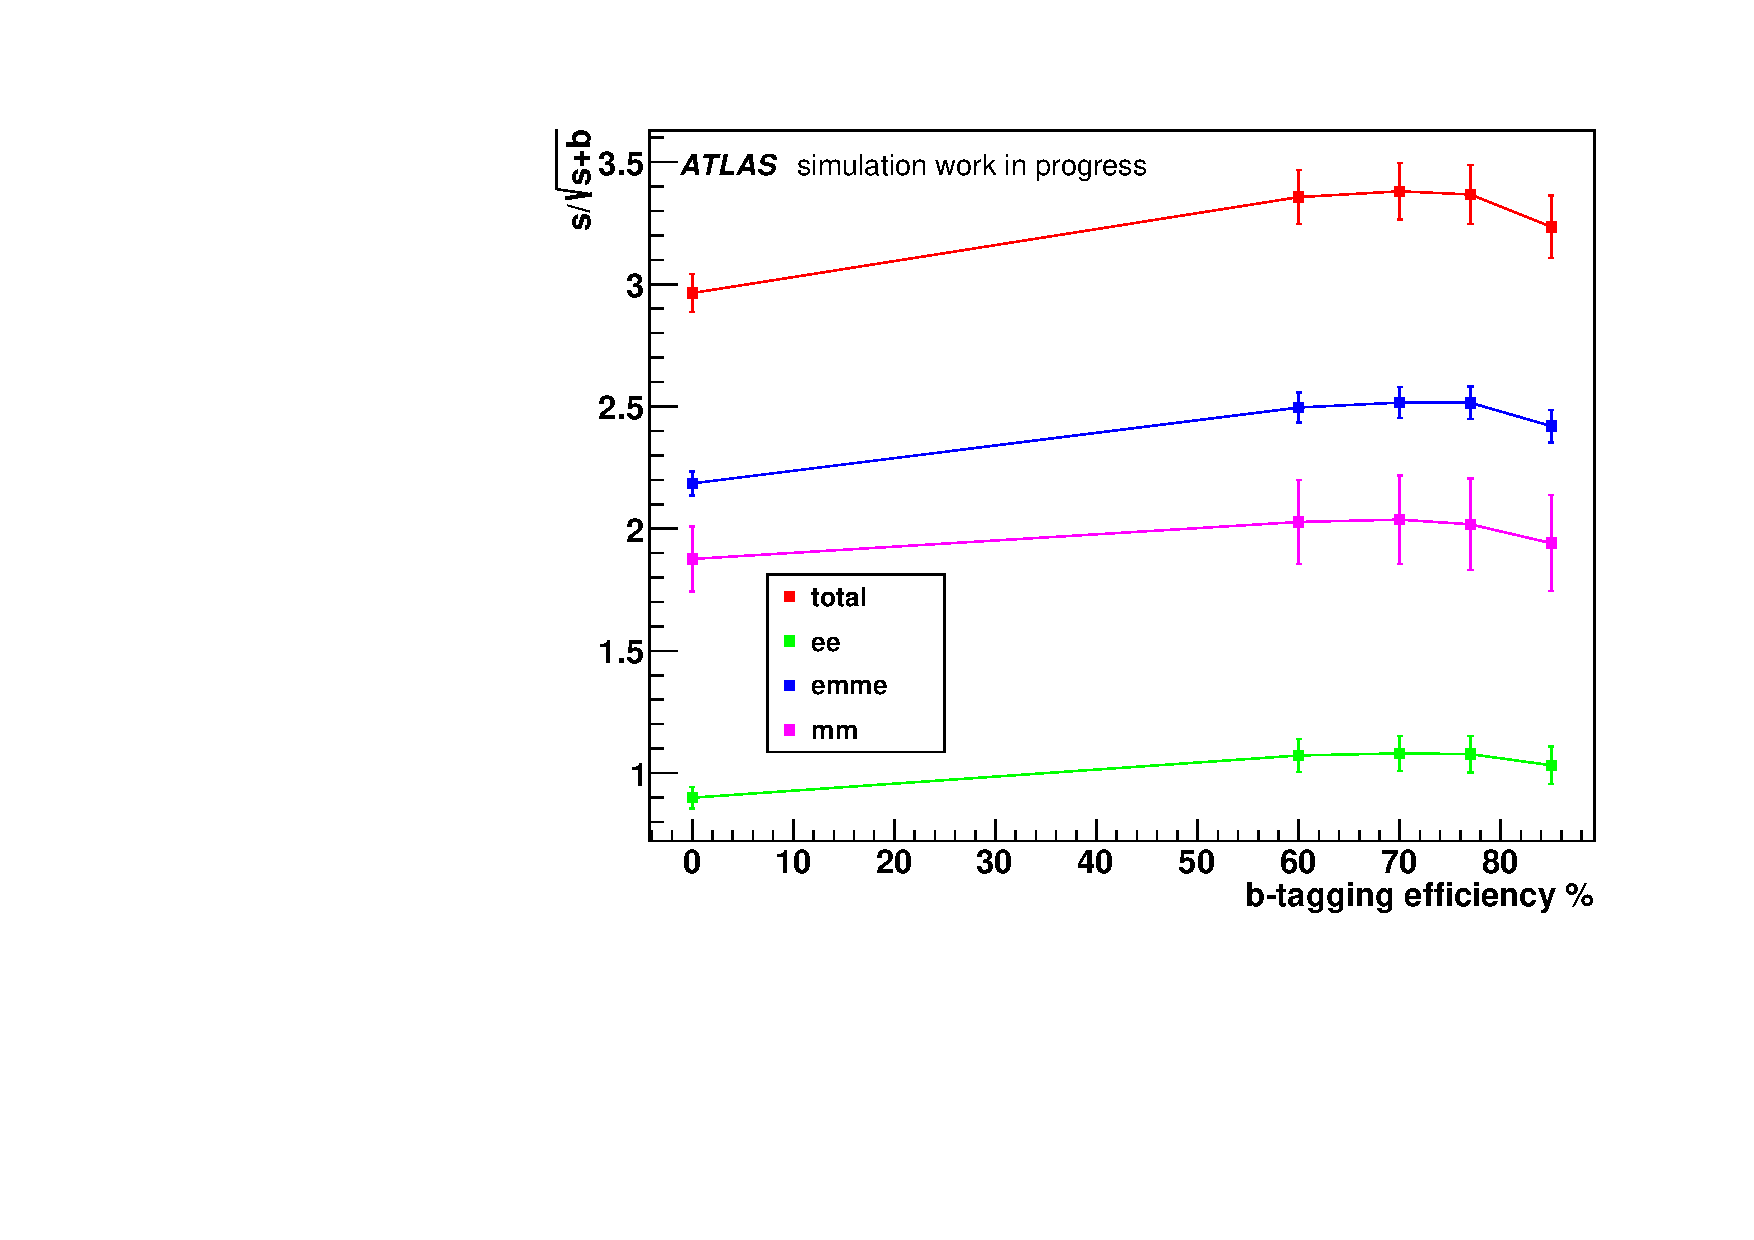
\includegraphics[width=1.\textwidth]{images/chapter7/noIso_stbr_btag_better.pdf}}
\caption{The significance at each multivariate $b$-tagger working point as well as the significance at $0\%$ (which corresponds to not using a $b$-jet veto at all). No isolation selection requirements were imposed on the lepton candidates.}
\label{optimal_b-tagging_working_point_noIso}
\end{figure}
\section{Optimising the Isolation Requirements for Lepton Candidates}
\subsection{The Cumulative Significance}
\label{description_of_cum_sig}
As stated in section \ref{intro_to_flb}, imposing an isolation requirement on the same-sign W-boson scattering lepton candidates is a technique for suppressing the \emph{fake lepton background}. The optimisation of the multivariate $b$-tagger was done by requiring candidate leptons to pass the \textit{Gradient} isolation selection working point (described in section \ref{iso_wps}). This section will be concerned with determining the optimal working point for the isolation selection; whether it be a fixed cut, a targeted efficiency such as \textit{Gradient}, or some composition of the two. Optimisation is based on the \emph{cumulative significance} quantity, defined as
$$
s_{cum}/\sqrt{s_{cum}+b_{cum}},
$$
where $s_{cum}$ is the sum of all signal events up to a given point being considered and similarly $b_{cum}$ is the sum of all background events up to that same point.

In order to determine how to use the cumulative significance to determine optimal analysis cuts, it is useful to plot it for a variety of artificial set-ups. However, first it is necessary to derive the uncertainty on the cumulative significance, in order to produce correct error bars necessary for comparison. For a function $f(x,y)$, the uncertainty is given by \cite{lyons}:
\begin{equation}
\sigma_{f}^{2} \approx \left| \frac{\partial f}{\partial x} \right| \sigma_{x}^{2} + \left| \frac{\partial f}{\partial y} \right| \sigma_{y}^{2}.
\end{equation}
Then if the cumulative significance is denoted $\alpha$, the uncertainty is:
\begin{equation}
\sigma_{\alpha}^{2} \approx \left| \frac{\partial \alpha}{\partial s_{cum}} \right| \sigma_{s_{cum}}^{2} + \left| \frac{\partial \alpha}{\partial b_{cum}} \right| \sigma_{b_{cum}}^{2}.
\end{equation}
Evaluating, gives:
\begin{equation}
\sigma_{\alpha}^{2} = \frac{s_{cum}+2b_{cum}}{2(s_{cum}+b_{cum})^{3/2}}\sigma_{s_{cum}}^{2} -\frac{s_{cum}}{2}\left( s_{cum} + b_{cum} \right)^{-3/2}\sigma_{b_{cum}}^{2},
\end{equation}
which is then used for the error bars subsequently.

Figures \ref{test_cum_sig} and \ref{test_cum_sig_rev} each display signal and background contributions for an arbitrary variable in a hypothetical experiment. In figure \ref{test_cum_sig}, the upper plots show two artificial set-ups where the signal contribution abruptly goes to zero at $x=6$, with the corresponding cumulative significance plotted below for each. In the upper right plot, the background contribution is constant at 25 across the entire $x$-range whereas the signal contribution is constant at 6 until the point $x=6$, after which it is zero. In the top left plot, the background contribution linearly increases whereas the signal contribution is constant at 6 until the point $x=6$ in the same way as the upper right plot. The cumulative significance of both the left and right set-ups peaks at the point where the signal goes to zero and then gradually decreases. This suggests placing an upper bound cut at $x = 6$ in order to maximise the cumulative significance.

Conversely, in figure \ref{test_cum_sig_rev}, the upper plots show two artificial set-ups where the signal contribution abruptly goes to 6 at $x=20$, with the corresponding cumulative significance plotted below for each. In the upper right plot, the background contribution is constant at 25 across the entire $x$-range whereas the signal contribution is constant at zero until the point $x=25$, after which it is 6. In the top left plot, the background contribution linearly decreases whereas the signal contribution is constant at zero until point $x=25$, in the same way as the upper right plot. The cumulative significance of both the left and right set-ups is zero until $x=25$, after which it grows rapidly. This suggests placing an lower bound cut at $x = 25$ in order to maximise the cumulative significance.

\begin{figure}\centering{
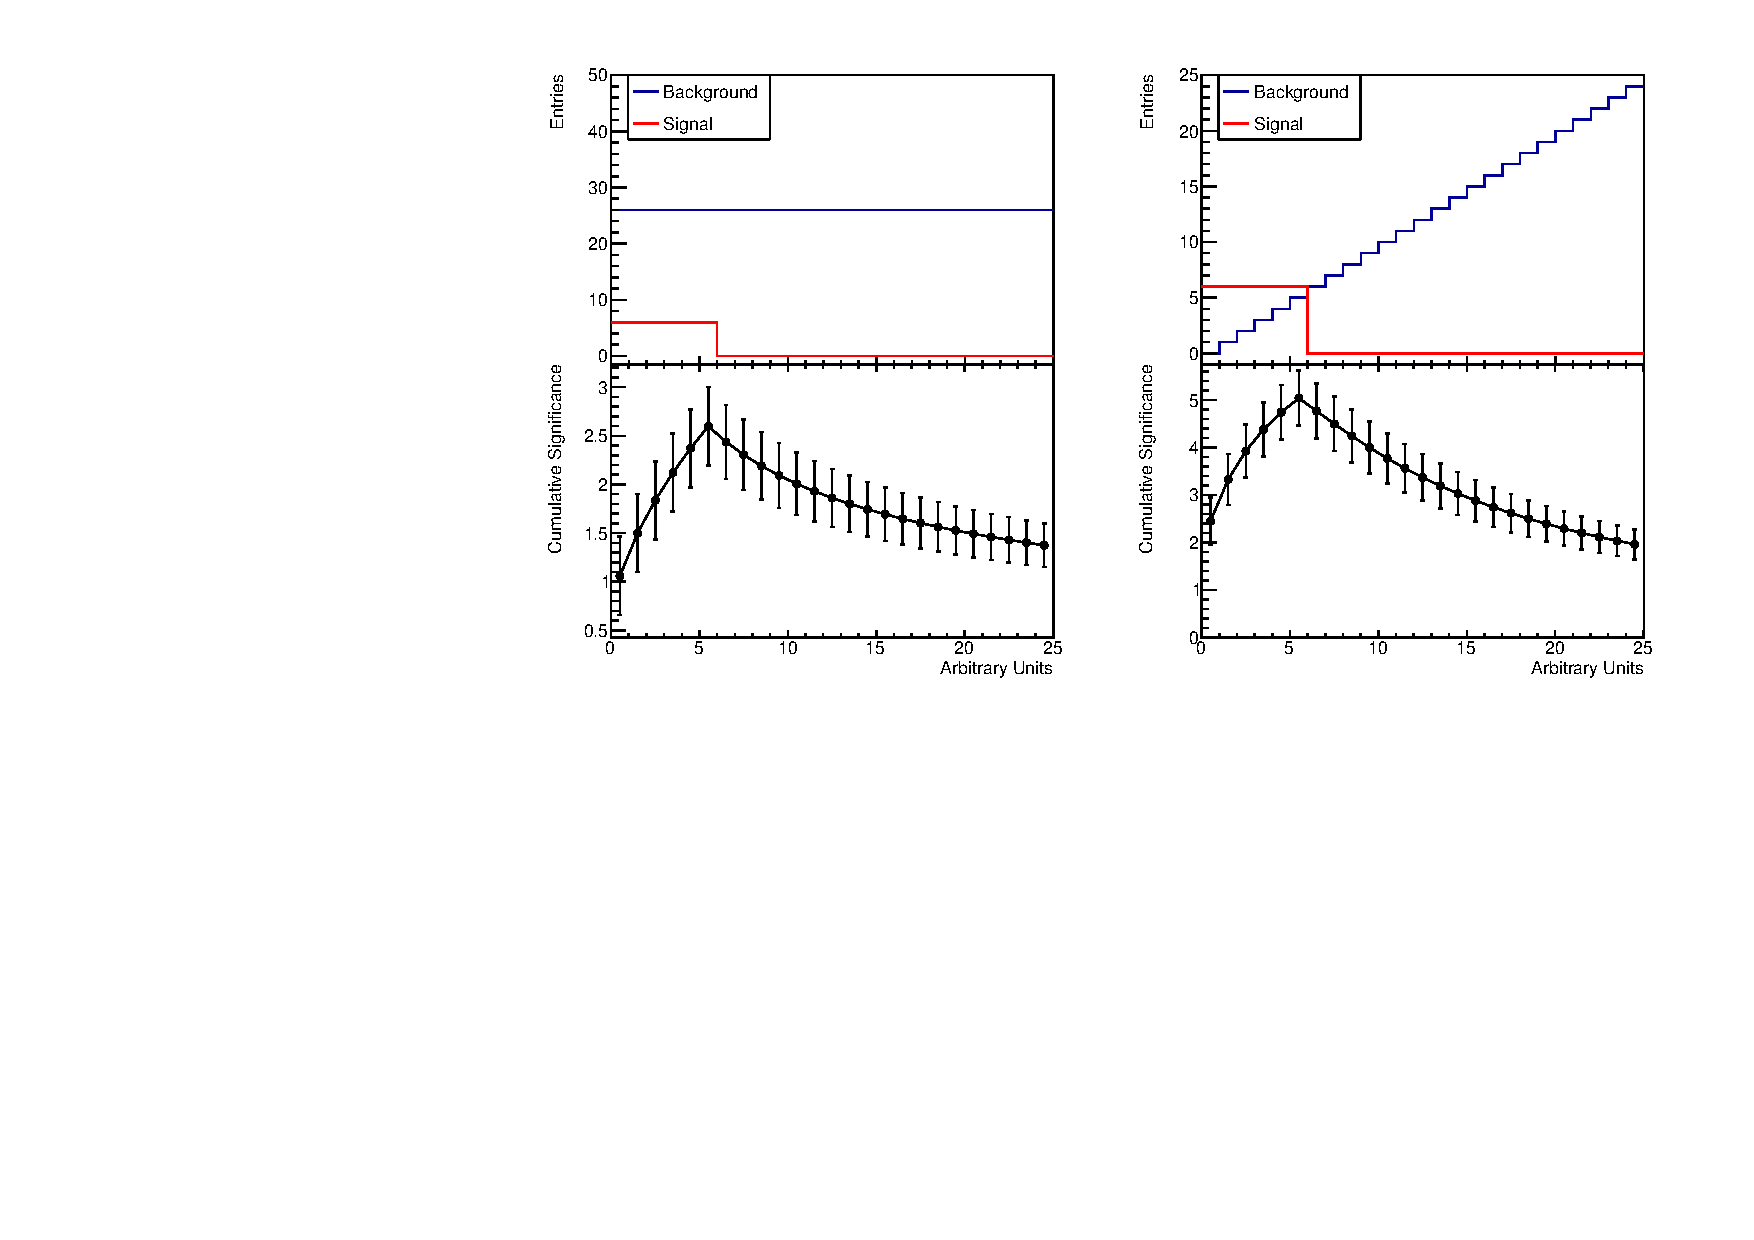
\includegraphics[width=1.\textwidth]{images/chapter7/test_cum_sig.pdf}
\caption{Two distinct artificial experimental setups, with the corresponding cumulative significances plotted below. Note the distinctive peak near $x=6$, indicating the optimal cut location.}
\label{test_cum_sig}
}\end{figure}
\begin{figure}\centering{
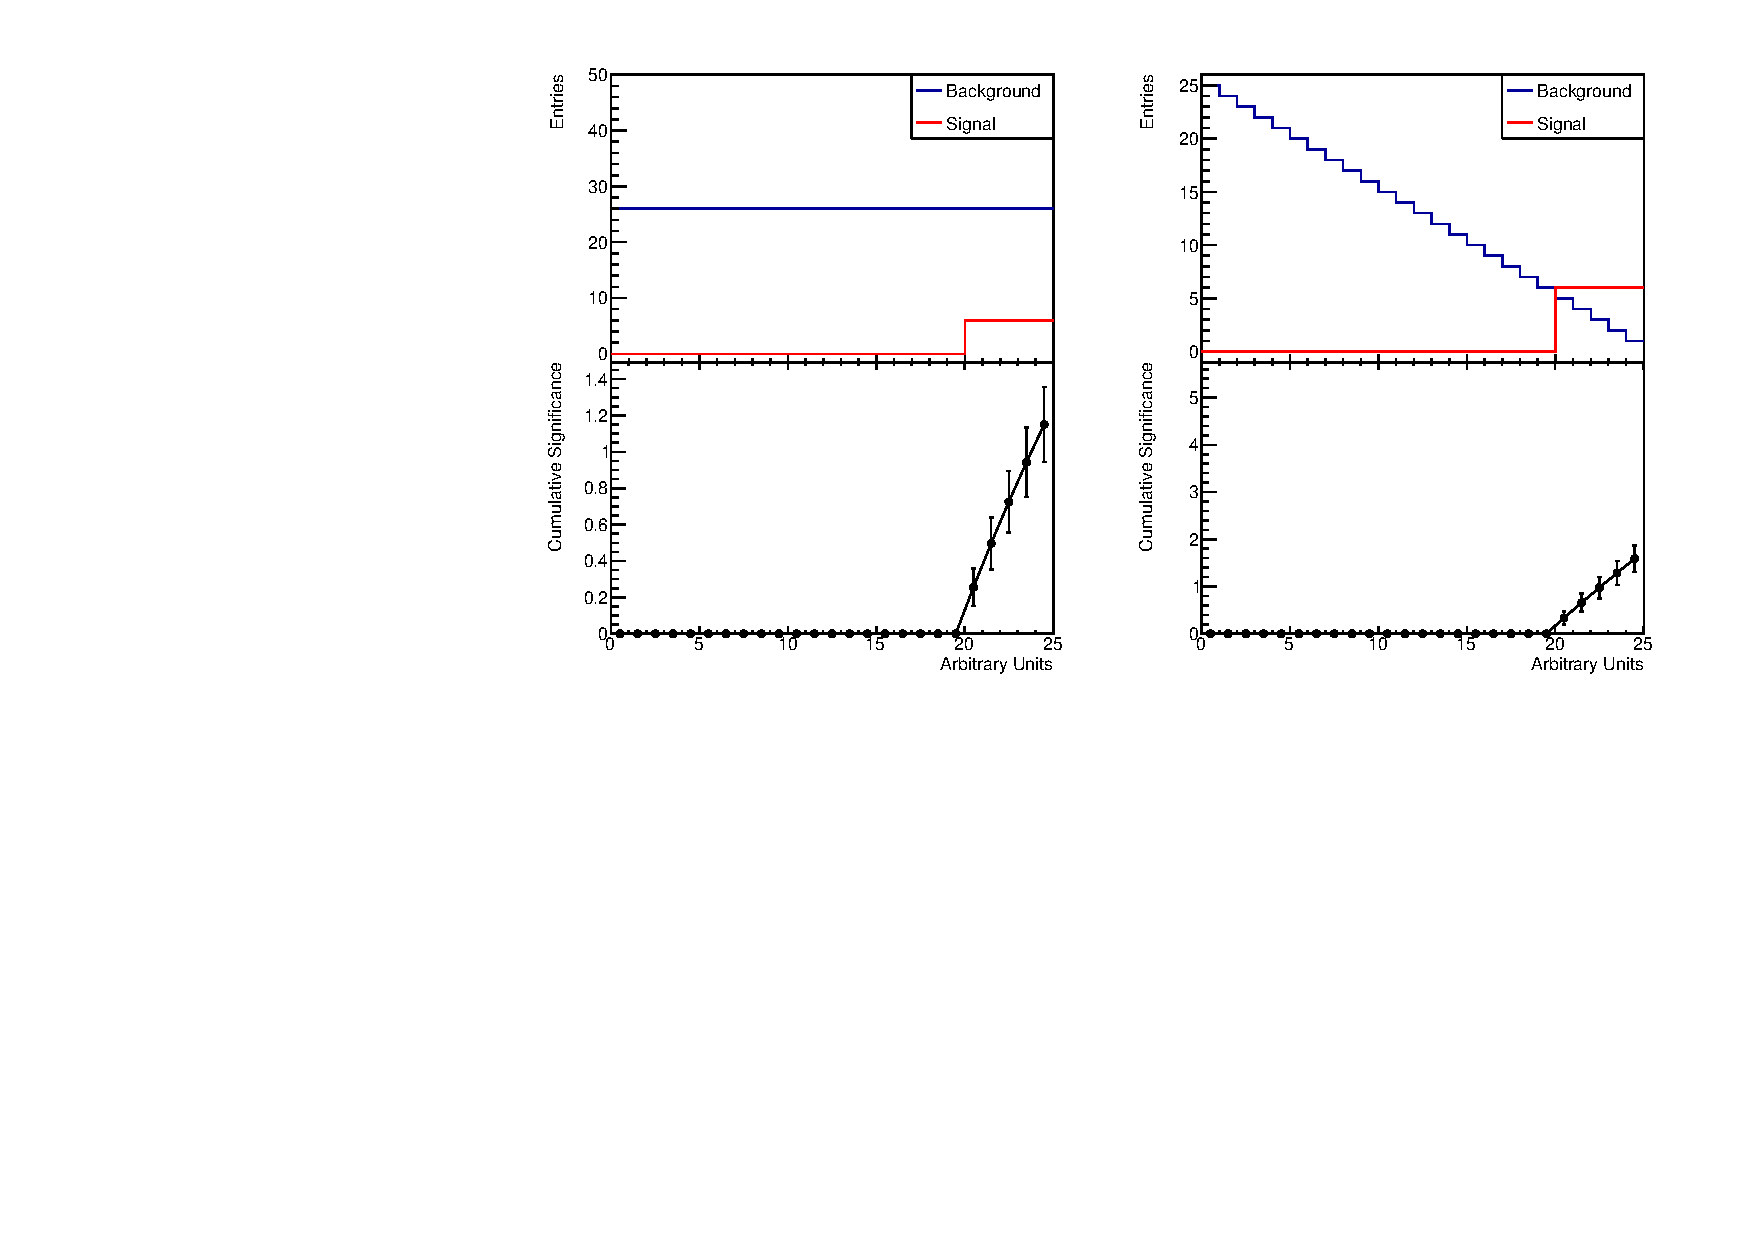
\includegraphics[width=1.\textwidth]{images/chapter7/test_cum_sig_rev.pdf}
\caption{Two distinct artificial experimental setups, with the corresponding cumulative significances plotted below. Note the rapid increase near $x=20$, indicating the optimal cut location.}
\label{test_cum_sig_rev}
}\end{figure}
\subsection{Determining the Optimal Isolation Selection Criteria}
\label{comparisons}
The cumulative significance can be used to optimise experimental analysis cuts. As was mentioned in section \ref{intro_to_flb}, isolation can be used to aid in the suppression of the \emph{fake lepton background}. The isolation selection tool used by ATLAS (see sub-section \ref{AIST}), provides two distinct classes of working points: fixed cuts and targeted efficiencies.

 In order to determine the optimal isolation selection requirement for the lepton candidates in same-sign W-boson scattering, the cumulative significances for the \textbf{topoetcone}, \textbf{fractional topoetcone}, \textbf{ptvarcone}, and \textbf{fractional ptvarcone} isolation variables were plotted. The variables prefixed by ``\textbf{fractional}'' are obtained by dividing the corresponding isolation variable of the physics object in question by its transverse momentum. Two sets of plots were produced. In the first set: lepton candidates were required to pass the targeted efficiency \textit{Gradient} isolation selection requirement. In the second set: the lepton candidates were not required to pass any isolation selection criteria. The aim of this study was to determine whether the optimal isolation requirement is: a fixed cut, \textit{Gradient}, or some composite cut combining elements of both. Given that these are plots of the cumulative significance, the value at a given point on the $x$-axis corresponds to the total significance of the events that would be gathered if a fixed cut was implemented at that point. For example, the cumulative significance of the $ee$-channel, \textbf{ptvarcone30}, no isolation selection requirement plot at the point $x = 1.0$ GeV, represents the total significance of all events included for analysis if a fixed-cut $\mathbf{ptvarcone30} < 1.0$ GeV was implemented. The same is true for the \textit{Gradient} isolation selection requirement plots, except that in this case considering the cumulative significance at some point corresponds to implementing a composite cut using both \textit{Gradient} isolation selection and a fixed-cut at the point in question. Regions where the no isolation selection requirement plots' cumulative significance is greater than the \textit{Gradient} isolation selection requirement plots' cumulative significance would suggest that a fixed-cut may perform better than \textit{Gradient} in this region. If a \textit{Gradient} isolation selection requirement plot achieves a maximum cumulative significance at a point other than that corresponding to the terminating bin, then this suggests cutting at this point to maximise the total significance of all events included for analysis.

In order to directly compare the two sets of plots, the cumulative significances for each variable in both sets were plotted together on the same set of axes, with the $ee$, $e\mu + \mu e$ , and $\mu\mu$ channels considered separately.  Only these plots produced for the direct comparison of the two sets are provided in this sub-section. For the individual plots of the cumulative significance, please see appendix \ref{appendix2}. Additionally, only the \textbf{cone30} isolation plots will be considered here, as this was the cone size used to set cuts on the variables in the Run 1 analysis. The \textbf{cone20} and \textbf{cone40} plots, for comparing the two different isolation selection requirements, display qualitatively the same behaviour as those examined here, and they are available in appendix \ref{appendix3}.

In the order of leading and sub-leading lepton respectively, figures: \ref{leading_topoetcone}, \ref{subleading_topoetcone} display the plots for the \textbf{topoetcone30} variable; figures: \ref{leading_frac-topoetcone} and \ref{subleading_frac-topoetcone} show the plots for \textbf{fractional topoetcone30} variable; figures: \ref{leading_ptvarcone}, \ref{subleading_ptvarcone} display the plots for the \textbf{ptvarcone30} variable; figures: \ref{leading_frac-ptvarcone} and \ref{subleading_frac-ptvarcone} show the plots for \textbf{fractional ptvarcone30} variable.

In general the lines for the channels, from the sub-leading lepton plots, with no isolation selection requirement, have a decrease in the cumulative significance in the terminating bin. The cumulative significances of the \textbf{topoetcone30} and \textbf{fractional topoetcone30} variables increase substantially from their starting values. This is in contrast to the \textbf{ptvarcone30} and \textbf{fractional ptvarcone30} plots, where there is very little variation in the cumulative significance except for the sub-leading lepton plots with the no isolation selection, where there is a noticeable dip in the terminating bin. These dips are due to the inclusion of overflow (mostly background) events in the final bins. The \textbf{topoetcone30} and \textbf{fractional topoetcone30} lines tend to have the channels from both the \textit{Gradient} selection and no isolation selection plots, display similar behaviour for low values of the variable but then subsequently diverge and become noticeably distinct with no overlap of the error bars.

Notice that at no point or $x$-range for any variable, channel, or leading or sub-leading lepton plot; do the solid lines corresponding to no isolation requirement, perform better than the dashed lines corresponding to the \textit{Gradient} isolation requirement. Note that the \textit{Gradient} isolation selection requirement is more effective for the $e\mu + \mu e$ and $\mu\mu$ channels where the difference between the two selections in very noticeable in all variables. In contrast, the effects on the plots in the $ee$-channel are very modest, with the errors bars overlapping, indicating that the effects are not statistically significant. This indicates that the \textit{Gradient} isolation selection requirement alone consistently performs better across all channels than any lone fixed-cut could. Although the effect is modest in the $ee$-channel.

The plots can be further interrogated to see if the cumulative significance of the dashed \textit{Gradient} isolation selection requirement lines, achieve maxima at points on the $x$-axis other than the terminating bin. This would indicate the a composite cut of using both the \textit{Gradient} isolation selection requirement with an additional fixed cut would be optimal. The $e\mu + \mu e$-channel line in figure \ref{leading_topoetcone}, the cumulative significance is seen to decrease in value in the terminating bin, so not all the \textit{Gradient} isolation selection requirement lines monotonically increase. Other lines, such as the $ee$-channel line in the same figure, show the cumulative significance achieving its maximum value at some intermediate point, in this case at $x \approx 3$. In all such cases however, the value of the cumulative significance in the terminating bin and at the maximum have overlapping errors bars. This indicates that the earlier maxima are not statically distinct from the values in the terminating bins. Hence, an additional fixed cut at these points would have a statistically negligible effect. Hence, the studies conclude that the optimal isolation requirement for lepton candidates is the \textit{Gradient} isolation requirement alone across all three channels, without any additional fixed cuts.
\begin{figure}
\centering
\begin{subfigure}{.85\textwidth}
  \centering
  \includegraphics[width=1.\linewidth]{../Desktop/workspace/l0-cone30/topoetcone30.pdf}
  \caption{}
  \label{leading_topoetcone}
\end{subfigure}
\begin{subfigure}{.85\textwidth}
  \centering
  \includegraphics[width=1.\linewidth]{../Desktop/workspace/l1-cone30/topoetcone30.pdf}
  \caption{}
  \label{subleading_topoetcone}
\end{subfigure}
\caption{Comparison of the \textbf{topoetcone30}-obtained cumulative significances for the leading (a) and sub-leading (b) lepton candidates; obtained for the case of requiring the leptons to pass the \textit{Gradient} isolation selection requirement (dashed lines) and for the case where the leptons are not required to pass any isolation selection requirement (solid lines).}
\label{comp_topoetcone}
\end{figure}
\begin{figure}
\centering
\begin{subfigure}{.85\textwidth}
  \centering
  \includegraphics[width=1.\linewidth]{../Desktop/workspace/l0-cone30/frac-topoetcone30.pdf}
  \caption{}
  \label{leading_frac-topoetcone}
\end{subfigure}
\begin{subfigure}{.85\textwidth}
  \centering
  \includegraphics[width=1.\linewidth]{../Desktop/workspace/l1-cone30/frac-topoetcone30.pdf}
  \caption{}
  \label{subleading_frac-topoetcone}
\end{subfigure}
\caption{Comparison of the \textbf{fractional-topoetcone30}-obtained cumulative significances for the leading (a) and sub-leading (b) lepton candidates; obtained for the case of requiring the leptons to pass the \textit{Gradient} isolation selection requirement (dashed lines) and for the case where the leptons are not required to pass any isolation selection requirement (solid lines).}
\label{comp_frac-topoetcone}
\end{figure}
\begin{figure}
\centering
\begin{subfigure}{.85\textwidth}
  \centering
  \includegraphics[width=1.\linewidth]{../Desktop/workspace/l0-cone30/ptvarcone30.pdf}
  \caption{}
  \label{leading_ptvarcone}
\end{subfigure}
\begin{subfigure}{.85\textwidth}
  \centering
  \includegraphics[width=1.\linewidth]{../Desktop/workspace/l1-cone30/ptvarcone30.pdf}
  \caption{}
  \label{subleading_ptvarcone}
\end{subfigure}
\caption{Comparison of the \textbf{ptvarcone30}-obtained cumulative significances for the leading (a) and sub-leading (b) lepton candidates; obtained for the case of requiring the leptons to pass the \textit{Gradient} isolation selection requirement (dashed lines) and for the case where the leptons are not required to pass any isolation selection requirement (solid lines).}
\label{comp_ptvarcone}
\end{figure}
\begin{figure}
\centering
\begin{subfigure}{.85\textwidth}
  \centering
  \includegraphics[width=1.\linewidth]{../Desktop/workspace/l0-cone30/frac-ptvarcone30.pdf}
  \caption{}
  \label{leading_frac-ptvarcone}
\end{subfigure}
\begin{subfigure}{.85\textwidth}
  \centering
  \includegraphics[width=1.\linewidth]{../Desktop/workspace/l1-cone30/frac-ptvarcone30.pdf}
  \caption{}
  \label{subleading_frac-ptvarcone}
\end{subfigure}
\caption{Comparison of the \textbf{fractional-ptvarcone30}-obtained cumulative significances for the leading (a) and sub-leading (b) lepton candidates; obtained for the case of requiring the leptons to pass the \textit{Gradient} isolation selection requirement (dashed lines) and for the case where the leptons are not required to pass any isolation selection requirement (solid lines).}
\label{comp_frac-ptvarcone}
\end{figure}
\section{Using the Cumulative Significance to Optimise Other Analysis Cuts}
The cumulative significance approach to analysis cut optimisation, described in sub-section \ref{description_of_cum_sig} and used in sub-section \ref{comparisons}, can also be used to optimise cuts on other variables. In this sub-section the cumulative significance approach is applied to three variables: the lepton invariant mass ($m_{\ell \ell}$), the jet invariant mass ($m_{jj}$), and the jet separation rapidity ($\Delta y_{jj}$). In each case the histogram and corresponding significance are plotted for the variable immediately before its associated cut is implemented. See section \ref{event_selection} for the ordered list of analysis cuts.

Figures \ref{ee_mll}, \ref{emme_mll}, and \ref{mm_mll} show the lepton invariant mass plots for the $ee$, $e\mu + \mu e$, and $\mu\mu$ channels respectively. While the $e \mu +\mu e$ plot suggests not implementing a cut at all\footnote{This is not in agreement with the current (as of writing) same-sign W-boson scattering analysis cut of: $m_{\ell \ell} > 20$ GeV, across all channels.}, both the $ee$ and $\mu\mu$ suggests cutting out the region $55 < m_{\ell \ell} < 95$ GeV. However, since the dominant background contributions are $Z$ + $jets$ events, and the mass spectrum peaks at the Z-mass of approximately 90 GeV, this can be interpreted as an argument to implement a Z-mass veto. This is done in a subsequent cut as listed in section \ref{event_selection} cut 5. which vetoes events failing: $76.2 < m_{ee} < 106.2$ GeV, only in the $ee$ channel.\footnote{Note that this mass region, cut out by the Z-mass veto, does not have the same bounds as the cut suggested by the looking at the cumulative significance. This is because the cumulative significance will dip and rise asymmetrically about the Z-mass peak at 91.2 GeV, in response to the sudden increases and then subsequent decreases in the number of background events.} This indicates that a Z-mass veto should also be imposed on $\mu\mu$-channel events.

Figures \ref{ee_mjj}, \ref{emme_mjj}, and \ref{mm_mjj} show the jet invariant mass plots for the $ee$, $e\mu + \mu e$, and $\mu\mu$ channels respectively; while figures \ref{ee_DYjj}, \ref{emme_DYjj}, \ref{mm_DYjj} show the jet separation rapidity plots in the same channel order. Note that the cumulative significances for both of these variables and for all channels suggest not implementing any associated cut. This is in opposition to current same-sign W-boson scattering analysis cuts on these variables of $m_{jj} > 500$ GeV and $\Delta y_{jj} > 2.4$.

\begin{figure}
	\centering
		\includegraphics[width = 0.5\textwidth]{../results/gamma/70_Grad_mc_only-ee/plots/ee-CutTriggerMatch-Mll-log.png}
		\caption{Histogram of the lepton invariant mass ($ee$ channel). The corresponding cumulative significance curve is plotted below.}
		\label{ee_mll}
\end{figure}
\begin{figure}
	\centering
		\includegraphics[width = 0.5\textwidth]{../results/gamma/70_Grad_mc_only-emme/plots/emme-CutTriggerMatch-Mll-log.png}
		\caption{Histogram of the lepton invariant mass ($e \mu + \mu e$ channel). The corresponding cumulative significance curve is plotted below.}
		\label{emme_mll}
\end{figure}
\begin{figure}
	\centering
		\includegraphics[width = 0.5\textwidth]{../results/gamma/70_Grad_mc_only-mm/plots/mm-CutTriggerMatch-Mll-log.png}
		\caption{Histogram of the lepton invariant mass ($\mu\mu$ channel). The corresponding cumulative significance curve is plotted below.}
		\label{mm_mll}
\end{figure}

\begin{figure}
	\centering
		\includegraphics[width = 0.5\textwidth]{../results/gamma/70_Grad_mc_only-ee/plots/ee-Cut2JSSBVeto-Mjj-lin.png}
		\caption{Histogram of the jet invariant mass ($ee$ channel). The corresponding cumulative significance curve is plotted below.}
		\label{ee_mjj}
\end{figure}
\begin{figure}
	\centering
		\includegraphics[width = 0.5\textwidth]{../results/gamma/70_Grad_mc_only-emme/plots/emme-Cut2JSSBVeto-Mjj-lin.png}
		\caption{Histogram of the jet invariant mass ($e \mu + \mu e$ channel). The corresponding cumulative significance curve is plotted below.}
		\label{emme_mjj}
\end{figure}
\begin{figure}
	\centering
		\includegraphics[width = 0.5\textwidth]{../results/gamma/70_Grad_mc_only-mm/plots/mm-Cut2JSSBVeto-Mjj-lin.png}
		\caption{Histogram of the jet invariant mass ($\mu\mu$ channel). The corresponding cumulative significance curve is plotted below.}
		\label{mm_mjj}
\end{figure}

\begin{figure}
	\centering
		\includegraphics[width = 0.5\textwidth]{../results/gamma/70_Grad_mc_only-ee/plots/ee-Cut2JSSMjj-DYjj-lin.png}
		\caption{Histogram of the jet separation rapidity ($ee$ channel). The corresponding cumulative significance curve is plotted below.}
		\label{ee_DYjj}
\end{figure}
\begin{figure}
	\centering
		\includegraphics[width = 0.5\textwidth]{../results/gamma/70_Grad_mc_only-emme/plots/emme-Cut2JSSMjj-DYjj-lin.png}
		\caption{Histogram of the jet separation rapidity ($e \mu + \mu e$ channel). The corresponding cumulative significance curve is plotted below.}
		\label{emme_DYjj}
\end{figure}
\begin{figure}
	\centering
		\includegraphics[width = 0.5\textwidth]{../results/gamma/70_Grad_mc_only-mm/plots/mm-Cut2JSSMjj-DYjj-lin.png}
		\caption{Histogram of the jet separation rapidity ($\mu\mu$ channel). The corresponding cumulative significance curve is plotted below.}
		\label{mm_DYjj}
\end{figure}

\chapter{Conclusion}
The scattering of W-bosons is a key process in probing electroweak symmetry breaking. In the absence of a Standard Model Higgs boson, the longitudinally polarised scattering amplitude of W-bosons scattering violates unitarity when the WW centre-of-mass energy exceeds approximately 1 TeV. A mechanism is required to unitarise this process. By adding the Standard Model Higgs boson, the cross section regains reasonable behaviour at high energies and the mathematical consistency of the Standard Model is preserved via the Higgs mechanism. A prompt lepton is defined as a lepton coming from a W-boson, while a non-prompt lepton is defined as coming from the decay of a hadron. Processes that contain non-prompt leptons form part of the background in events selected for the same sign W-boson scattering measurement. These non-prompt leptons are called the `fake lepton background'. The dominant contribution to the fake lepton background is from the process:$t\bar{t} \longrightarrow WbWb \longrightarrow \ell \nu  bb qq$.

In this thesis, two strategies for suppressing the fake lepton background were optimised. Optimisation studies on the ATLAS Run 2 multivariate b-tagger suggest moving the working point from the current 85$\%$ efficiency, currently used by the ATLAS Run 2 same-sign W-boson scattering analysis, to the 70$\%$ efficiency in order to maximise the significance. However, due to the fact that the effect on increasing the significance may be a statistical fluctuation, more studies using larger sample sizes should be conducted before recommending the change.  It was also determined that the \textit{Gradient} isolation selection working point was the optimal requirement that can be imposed on signal lepton candidates; no additional fixed cut on the \textbf{topoetcone} or \textbf{ptvarcone} isolation variables is necessary. The isolation requirement was optimised using the cumulative significance quantity, which was first tested in order to anticipate its usefulness for determining cuts on analysis variables.

This approach using the cumulative significance was then applied to three other analysis cuts: the lepton invariant mass $m_{\ell \ell}$, the jet invariant mass $m_{jj}$, and the jet rapidity separation $\Delta y_{jj}$. The advantage of implementing a Z-mass veto on the $ee$-channel was confirmed by examining the cumulative significance of $m_{\ell \ell}$. This examination also indicated that a Z-mass veto should also be implemented on the $\mu\mu$-channel. The studies indicated that jet invariant mass, jet rapidity separation, and $m_{\ell \ell}$ ($e\mu + \mu e$)-channel do not require cuts. These cut optimisations are not in agreement with those utilised for the ATLAS Run 1 same-sign W-boson scattering analysis. It is possible that the Monte Carlo simulated data being used for the optimisation in this thesis is not accurately modeling the same-sign W-boson scattering process or one or more of the background processes. Further analysis using additional MC samples is needed in order to vindicate or dismiss the cut recommendations on the $m_{\ell \ell}$, $m_{jj}$, and  $\Delta y_{jj}$ variable. Additionally, the effects of the recomendations on actual LHC data recorded by the ATLAS detector could be insightful as to whether they are advantageous.

%now enable appendix numbering format and include any appendices
\appendix
\chapter{Gauge Theories}
\label{appendix1}
This section is adapted from \cite{griffiths}.

The Lagrangian formulation of classical mechanics has at its core the \emph{Euler-Lagrange} equations:
\begin{equation}
\frac{d}{dt} \left( \frac{\partial \mathcal{L}}{\partial \dot{q_{j}}} \right) = \frac{\partial \mathcal{L}}{\partial q_{j}} \ \ \ \ \ \ \ \ \ \ \ \ (j=1,2,3,...),
\end{equation}
where $ \mathcal{L} = T - U$, $T$ is the kinetic energy of the particle, $U$ is a scalar potential energy, and $q_{j}$ are the generalised coordinates.

In relativistic field theory space and time must be treated equally and the Euler-Lagrange equations generalise to:
\begin{equation}
\partial _{\mu} \left( \frac{\partial \mathcal{L}}{\partial \left( \partial_{\mu} \phi_{i} \right)} \right) = \frac{\partial \mathcal{L}}{\partial \phi_{i}} \ \ \ \ \ \ \ \ \ \ \ \ (i=1,2,3,...),
\end{equation}
where $\phi _{i}$ are the field variables which are now functions of space and time.

The Lagrangian in relativistic field theories is usually taken to be axiomatic, in contrast to how it is usually derived classically. As an example consider the \emph{Dirac Lagrangian}:
\begin{equation}
\mathcal{L} = i \bar{\psi} \gamma _{\mu} \partial_{\mu} \psi - m \bar{\psi} \psi,
\end{equation}
where $\psi$ is a spinor field, $\bar{\psi}$ its adjoint, and $\gamma ^{\mu}$ the gamma matrices. Inserting this into the generalised Euler-Lagrange equations produces the \emph{Dirac equation}, which describes a massive spin-1/2 particle. Note that the Dirac Lagrangian is invariant under what is called a \emph{global phase transformation}: 
\begin{equation}
\psi \longrightarrow e^{i \theta} \psi,
\label{gpt}
\end{equation}
where the phase factor $\theta \in \mathbb{R}$. However if the phase factor in the transformation is given spatial dependence:
\begin{equation}
 \psi \longrightarrow e^{i \theta (x)} \psi,
\end{equation} 
in what is called now called a \emph{local phase transformation}, then the Lagrangian is no longer invariant since:
$$
\partial_{\mu} \left( e^{i \theta (x)} \psi \right) = i \left( \partial_{\mu} \theta(x) \right) e^{i \theta(x)} \psi + e^{i \theta (x)}\partial_{\mu} \psi.
$$
Defining now: 
\begin{equation}
\lambda (x) = - \frac{\theta(x)}{q},
\end{equation}
where q is the charge of the particle in question, then the local phase transformation becomes:
\begin{equation}
\psi \longrightarrow e^{-iq\lambda (x)}\psi,
\end{equation}
and the Lagrangian gains an extra term when subjected to a local phase transformation:
\begin{equation}
\mathcal{L} \longrightarrow \mathcal{L} + \left( q \bar{\psi}\gamma^{\mu} \psi \right) \partial_{\mu}\lambda
\end{equation}
Introduce the vector field $A_{\mu}$ that transforms under a local phase transformation according to:
\begin{equation}
A_{\mu} \longrightarrow A_{\mu} + \partial_{\mu} \lambda.
\label{vf lpt}
\end{equation}
The Dirac Lagrangian can thus be modified to be invariant under a local phase transformation by adding a term:
\begin{equation}
\mathcal{L} = \left[ i \bar{\psi} \gamma^{\mu} \partial_{\mu} \psi - m \bar{\psi} \psi \right] - \left( q \bar{\psi} \gamma^{\mu} \psi \right) A_{\mu}.
\end{equation}
The last term has the interpretation of the vector field $A_{\mu}$ coupling to the field $\psi$. The full Lagrangian should also contain a free term for $A_{\mu}$. Comparing to the Proca Lagrangian\footnote{When entered into the Euler-Lagrange equations, the Proca Lagrangian yields the Proca equation (which describes a massive particle of spin-1).}:
\begin{equation}
\mathcal{L} = \frac{-1}{16 \pi} F^{\mu \nu} F_{\mu \nu} + \frac{1}{8 \pi} \left( m_{A} \right)^{2} A^{\nu} A_{\nu},
\end{equation}
where $m_{A}$ is the mass of the vector field and 
\begin{equation}
F^{\mu \nu} = \left( \partial^{\mu} A^{\nu} - \partial^{\nu} A^{\mu} \right).
\end{equation}
$F{\mu \nu}$ is the field strength tensor and it is invariant under a local phase transformation, however $A^{\nu}A_{\nu}$ isn't unless $m_{A} = 0$. Thus in order for the free term to be invariant under a local phase transformation, the vector field must be massless. If this is interpreted in the context of electrodynamics then $A^{\mu}$ is the electromagnetic potential and equations \ref{gpt} and \ref{vf lpt} are gauge transformations analogous to the ones found in classical electrodynamics. Additionally, in this context, vector fields such as $A^{\mu}$ are commonly referred to as gauge fields.

The local phase invariance can be regained by replacing the derivatives $\partial_{\mu}$ with so-called \emph{covariant derivatives}:
\begin{equation}
D_{\mu} \equiv \partial_{\mu} + iqA_{\mu},
\end{equation}
as this will cancel the extra term introduced in equation \ref{vf lpt} such that:
\begin{equation}
D_{\mu} \psi \longrightarrow e^{iq \lambda} D_{\mu} \psi,
\end{equation}
and the Lagrangian will now be local phase invariant.

The gauge transformations can be thought of as multiplication of the field $\psi$ by a unitary $1 \times 1$ matrix:
\begin{equation}
\psi \longrightarrow U \psi,
\end{equation}
where $ U = e^{i \theta}$. This Quantum Field Theory (QFT) is an example of what is commonly referred to as a \emph{gauge theory}. Gauge theories are a special class of QFTs that are closely associated with a particular symmetry group. In the case here the symmetry group is $\mathbf{U}(1)$. Such symmetry groups can be either abelian (as is the case here) or non-abelian.\footnote{Gauge theories that are associated with non-abelian symmetry groups are commonly referred to as Yang-Mills theories; e.g. in QCD the symmetry group is the non-abelian $SU(3)$, as such QCD is a Yang-Mills theory.}

The field variables in a Standard Model gauge theory are interpreted as being quantised, with the quanta of the fields being particles. Hence, the quantum of the electromagnetic field $A^{\mu}$ is the photon, leptons and quarks are associated with Dirac fields, gluons are the quanta of the eight $\mathbf{SU}(3)$ gauge fields of QCD, and the W and Z bosons are the quanta of associated Proca fields. In particular, the quanta of the gauge fields are the gauge bosons; spin-1 particles which mediate the interaction associated with their field.
\chapter{Plots of the Isolation Variables}
\label{appendix2}
A sample plot of each cone30 variable, for both cases is shown in this section. For each plot of an isolation variable, the corresponding cumulative significance is plotted below on the same $x$-axis. The intermediate cone size, the cone30 isolation variables will be considered in this appendix. The cone20 and cone40 plots display qualitatively the same behaviour. Each Figure contains a sub-figure showing the plot for the leading lepton (a), and another for the sub-leading lepton (b).
\begin{figure}
\centering
\begin{subfigure}{.65\textwidth}
  \centering
  \includegraphics[width=1.\linewidth]{../results/alpha/70_Grad_mc_only-ee/plots/ee-Cut2JSSSR-l0_topoetcone30-lin.png}
  \caption{}
  \label{ee_eading_topoetcone}
\end{subfigure}
\begin{subfigure}{.65\textwidth}
 \centering
  \includegraphics[width=1.\linewidth]{../results/alpha/70_Grad_mc_only-ee/plots/ee-Cut2JSSSR-l1_topoetcone30-lin.png}
  \caption{}
  \label{ee_subleading_topoetcone}
\end{subfigure}
\caption{Histograms of \textbf{topoetcone30} for the leading (a) and sub-leading (b) $ee$-channel leptons. The corresponding plots of the cumulative significance are displayed below each histogram. The leptons are required to pass the \textit{Gradient} isolation requirement. Overflow contained in terminating bin.}
\label{topoetcone30_isoplots_wGrad_ee}
\end{figure}
\begin{figure}
\centering
\begin{subfigure}{.65\textwidth}
  \centering
  \includegraphics[width=1.\linewidth]{../results/alpha/70_Grad_mc_only-emme/plots/emme-Cut2JSSSR-l0_topoetcone30-lin.png}
  \caption{}
  \label{emme_leading_topoetcone}
\end{subfigure}
\begin{subfigure}{.65\textwidth}
 \centering
  \includegraphics[width=1.\linewidth]{../results/alpha/70_Grad_mc_only-emme/plots/emme-Cut2JSSSR-l1_topoetcone30-lin.png}
  \caption{}
  \label{emme_subleading_topoetcone}
\end{subfigure}
\caption{Histograms of \textbf{topoetcone30} for the leading (a) and sub-leading (b) $e\mu+\mu e$-channel leptons. The corresponding plots of the cumulative significance are displayed below each histogram. The leptons are required to pass the \textit{Gradient} isolation requirement. Overflow contained in terminating bin.}
\label{topoetcone30_isoplots_wGrad_emme}
\end{figure}
\begin{figure}
\centering
\begin{subfigure}{.65\textwidth}
  \centering
  \includegraphics[width=1.\linewidth]{../results/alpha/70_Grad_mc_only-mm/plots/mm-Cut2JSSSR-l0_topoetcone30-lin.png}
  \caption{}
  \label{mm_leading_topoetcone}
\end{subfigure}
\begin{subfigure}{.65\textwidth}
 \centering
  \includegraphics[width=1.\linewidth]{../results/alpha/70_Grad_mc_only-mm/plots/mm-Cut2JSSSR-l1_topoetcone30-lin.png}
  \caption{}
  \label{mm_subleading_topoetcone}
\end{subfigure}
\caption{Histograms of \textbf{topoetcone30} for the leading (a) and sub-leading (b) $\mu\mu$-channel leptons. The corresponding plots of the cumulative significance are displayed below each histogram. The leptons are required to pass the \textit{Gradient} isolation requirement. Overflow contained in terminating bin.}
\label{topoetcone30_isoplots_wGrad_mm}
\end{figure}
\begin{figure}
\centering
\begin{subfigure}{.65\textwidth}
  \centering
  \includegraphics[width=1.\linewidth]{../results/alpha/70_Grad_mc_only-ee/plots/ee-Cut2JSSSR-l0_ftopoetcone30-lin.png}
  \caption{}
  \label{ee_leading_topoetcone}
\end{subfigure}
\begin{subfigure}{.65\textwidth}
 \centering
  \includegraphics[width=1.\linewidth]{../results/alpha/70_Grad_mc_only-ee/plots/ee-Cut2JSSSR-l1_ftopoetcone30-lin.png}
  \caption{}
  \label{ee_subleading_topoetcone}
\end{subfigure}
\caption{Histograms of \textbf{fractional-topoetcone30} for the leading (a) and sub-leading (b) $ee$-channel leptons. The corresponding plots of the cumulative significance are displayed below each histogram. The leptons are required to pass the \textit{Gradient} isolation requirement. Overflow contained in terminating bin.}
\label{ftopoetcone30_isoplots_wGrad_ee}
\end{figure}
\begin{figure}
\centering
\begin{subfigure}{.65\textwidth}
  \centering
  \includegraphics[width=1.\linewidth]{../results/alpha/70_Grad_mc_only-emme/plots/emme-Cut2JSSSR-l0_ftopoetcone30-lin.png}
  \caption{}
  \label{emme_leading_topoetcone}
\end{subfigure}
\begin{subfigure}{.65\textwidth}
 \centering
  \includegraphics[width=1.\linewidth]{../results/alpha/70_Grad_mc_only-emme/plots/emme-Cut2JSSSR-l1_ftopoetcone30-lin.png}
  \caption{}
  \label{emme_subleading_topoetcone}
\end{subfigure}
\caption{Histograms of \textbf{fractional-topoetcone30} for the leading (a) and sub-leading (b) $e\mu+\mu e$-channel leptons. The corresponding plots of the cumulative significance are displayed below each histogram. The leptons are required to pass the \textit{Gradient} isolation requirement. Overflow contained in terminating bin.}
\label{ftopoetcone30_isoplots_wGrad_emme}
\end{figure}
\begin{figure}
\centering
\begin{subfigure}{.65\textwidth}
  \centering
  \includegraphics[width=1.\linewidth]{../results/alpha/70_Grad_mc_only-mm/plots/mm-Cut2JSSSR-l0_ftopoetcone30-lin.png}
  \caption{}
  \label{mm_leading_topoetcone}
\end{subfigure}
\begin{subfigure}{.65\textwidth}
 \centering
  \includegraphics[width=1.\linewidth]{../results/alpha/70_Grad_mc_only-mm/plots/mm-Cut2JSSSR-l1_ftopoetcone30-lin.png}
  \caption{}
  \label{mm_subleading_topoetcone}
\end{subfigure}
\caption{Histograms of \textbf{fractional-topoetcone30} for the leading (a) and sub-leading (b) $\mu\mu$-channel leptons. The corresponding plots of the cumulative significance are displayed below each histogram. The leptons are required to pass the \textit{Gradient} isolation requirement. Overflow contained in terminating bin.}
\label{ftopoetcone30_isoplots_wGrad_mm}
\end{figure}
\begin{figure}
\centering
\begin{subfigure}{.65\textwidth}
  \centering
  \includegraphics[width=1.\linewidth]{../results/alpha/70_noIso_mc_only-ee/plots/ee-Cut2JSSSR-l0_topoetcone30-lin.png}
  \caption{}
  \label{ee_leading_topoetcone}
\end{subfigure}
\begin{subfigure}{.65\textwidth}
 \centering
  \includegraphics[width=1.\linewidth]{../results/alpha/70_noIso_mc_only-ee/plots/ee-Cut2JSSSR-l1_topoetcone30-lin.png}
  \caption{}
  \label{ee_subleading_topoetcone}
\end{subfigure}
\caption{Histograms of \textbf{topoetcone30} for the leading (a) and sub-leading (b) $ee$-channel leptons. The corresponding plots of the cumulative significance are displayed below each histogram. The leptons are not subjected to any isolation requirement. Overflow contained in terminating bin.}
\label{topoetcone30_isoplots_noIso_ee}
\end{figure}
\begin{figure}
\centering
\begin{subfigure}{.65\textwidth}
  \centering
  \includegraphics[width=1.\linewidth]{../results/alpha/70_noIso_mc_only-emme/plots/emme-Cut2JSSSR-l0_topoetcone30-lin.png}
  \caption{}
  \label{emme_leading_topoetcone}
\end{subfigure}
\begin{subfigure}{.65\textwidth}
 \centering
  \includegraphics[width=1.\linewidth]{../results/alpha/70_noIso_mc_only-emme/plots/emme-Cut2JSSSR-l1_topoetcone30-lin.png}
  \caption{}
  \label{emme_subleading_topoetcone}
\end{subfigure}
\caption{Histograms of \textbf{topoetcone30} for the leading (a) and sub-leading (b) $e\mu+\mu e$-channel leptons. The corresponding plots of the cumulative significance are displayed below each histogram. The leptons are not subjected to any isolation requirement. Overflow contained in terminating bin.}
\label{topoetcone30_isoplots_noIso_emme}
\end{figure}
\begin{figure}
\centering
\begin{subfigure}{.65\textwidth}
  \centering
  \includegraphics[width=1.\linewidth]{../results/alpha/70_noIso_mc_only-mm/plots/mm-Cut2JSSSR-l0_topoetcone30-lin.png}
  \caption{}
  \label{mm_leading_topoetcone}
\end{subfigure}
\begin{subfigure}{.65\textwidth}
 \centering
  \includegraphics[width=1.\linewidth]{../results/alpha/70_noIso_mc_only-mm/plots/mm-Cut2JSSSR-l1_topoetcone30-lin.png}
  \caption{}
  \label{mm_subleading_topoetcone}
\end{subfigure}
\caption{Histograms of \textbf{topoetcone30} for the leading (a) and sub-leading (b) $\mu\mu$-channel leptons. The corresponding plots of the cumulative significance are displayed below each histogram. The leptons are not subjected to any isolation requirement. Overflow contained in terminating bin.}
\label{topoetcone30_isoplots_noIso_mm}
\end{figure}
\begin{figure}
\centering
\begin{subfigure}{.65\textwidth}
  \centering
  \includegraphics[width=1.\linewidth]{../results/alpha/70_noIso_mc_only-ee/plots/ee-Cut2JSSSR-l0_ftopoetcone30-lin.png}
  \caption{}
  \label{ee_leading_topoetcone}
\end{subfigure}
\begin{subfigure}{.65\textwidth}
 \centering
  \includegraphics[width=1.\linewidth]{../results/alpha/70_noIso_mc_only-ee/plots/ee-Cut2JSSSR-l1_ftopoetcone30-lin.png}
  \caption{}
  \label{ee_subleading_topoetcone}
\end{subfigure}
\caption{Histograms of \textbf{fractional-topoetcone30} for the leading (a) and sub-leading (b) $ee$-channel leptons. The corresponding plots of the cumulative significance are displayed below each histogram. The leptons are not subjected to any isolation requirement. Overflow contained in terminating bin.}
\label{ftopoetcone30_isoplots_noIso_ee}
\end{figure}
\begin{figure}
\centering
\begin{subfigure}{.65\textwidth}
  \centering
  \includegraphics[width=1.\linewidth]{../results/alpha/70_noIso_mc_only-emme/plots/emme-Cut2JSSSR-l0_ftopoetcone30-lin.png}
  \caption{}
  \label{emme_leading_topoetcone}
\end{subfigure}
\begin{subfigure}{.65\textwidth}
 \centering
  \includegraphics[width=1.\linewidth]{../results/alpha/70_noIso_mc_only-emme/plots/emme-Cut2JSSSR-l1_ftopoetcone30-lin.png}
  \caption{}
  \label{emme_subleading_topoetcone}
\end{subfigure}
\caption{Histograms of \textbf{fractional-topoetcone30} for the leading (a) and sub-leading (b) $e\mu+\mu e$-channel leptons. The corresponding plots of the cumulative significance are displayed below each histogram. The leptons are not subjected to any isolation requirement. Overflow contained in terminating bin.}
\label{ftopoetcone30_isoplots_noIso_emme}
\end{figure}
\begin{figure}
\centering
\begin{subfigure}{.65\textwidth}
  \centering
  \includegraphics[width=1.\linewidth]{../results/alpha/70_noIso_mc_only-mm/plots/mm-Cut2JSSSR-l0_ftopoetcone30-lin.png}
  \caption{}
  \label{mm_leading_topoetcone}
\end{subfigure}
\begin{subfigure}{.65\textwidth}
 \centering
  \includegraphics[width=1.\linewidth]{../results/alpha/70_noIso_mc_only-mm/plots/mm-Cut2JSSSR-l1_ftopoetcone30-lin.png}
  \caption{}
  \label{mm_subleading_topoetcone}
\end{subfigure}
\caption{Histograms of \textbf{fractional-topoetcone30} for the leading (a) and sub-leading (b) $\mu\mu$-channel leptons. The corresponding plots of the cumulative significance are displayed below each histogram. The leptons are not subjected to any isolation requirement. Overflow contained in terminating bin.}
\label{ftopoetcone30_isoplots_noIso_mm}
\end{figure}
\begin{figure}
\centering
\begin{subfigure}{.65\textwidth}
  \centering
  \includegraphics[width=1.\linewidth]{../results/alpha/70_Grad_mc_only-ee/plots/ee-Cut2JSSSR-l0_ptvarcone30-log.png}
  \caption{}
  \label{ee_leading_topoetcone}
\end{subfigure}
\begin{subfigure}{.65\textwidth}
 \centering
  \includegraphics[width=1.\linewidth]{../results/alpha/70_Grad_mc_only-ee/plots/ee-Cut2JSSSR-l1_ptvarcone30-log.png}
  \caption{}
  \label{ee_subleading_topoetcone}
\end{subfigure}
\caption{Histograms of \textbf{ptvarcone30} for the leading (a) and sub-leading (b) $ee$-channel leptons. The corresponding plots of the cumulative significance are displayed below each histogram. The leptons are required to pass the \textit{Gradient} isolation requirement. Overflow contained in terminating bin.}
\label{ptvarcone30_isoplots_wGrad_ee}
\end{figure}
\begin{figure}
\centering
\begin{subfigure}{.65\textwidth}
  \centering
  \includegraphics[width=1.\linewidth]{../results/alpha/70_Grad_mc_only-emme/plots/emme-Cut2JSSSR-l0_ptvarcone30-log.png}
  \caption{}
  \label{emme_leading_topoetcone}
\end{subfigure}
\begin{subfigure}{.65\textwidth}
 \centering
  \includegraphics[width=1.\linewidth]{../results/alpha/70_Grad_mc_only-emme/plots/emme-Cut2JSSSR-l1_ptvarcone30-log.png}
  \caption{}
  \label{emme_subleading_topoetcone}
\end{subfigure}
\caption{Histograms of \textbf{ptvarcone30} for the leading (a) and sub-leading (b) $e\mu+ \mu e$-channel leptons. The corresponding plots of the cumulative significance are displayed below each histogram. The leptons are required to pass the \textit{Gradient} isolation requirement. Overflow contained in terminating bin.}
\label{ptvarcone30_isoplots_wGrad_emme}
\end{figure}
\begin{figure}
\centering
\begin{subfigure}{.65\textwidth}
  \centering
  \includegraphics[width=1.\linewidth]{../results/alpha/70_Grad_mc_only-mm/plots/mm-Cut2JSSSR-l0_ptvarcone30-log.png}
  \caption{}
  \label{mm_leading_topoetcone}
\end{subfigure}
\begin{subfigure}{.65\textwidth}
 \centering
  \includegraphics[width=1.\linewidth]{../results/alpha/70_Grad_mc_only-mm/plots/mm-Cut2JSSSR-l1_ptvarcone30-log.png}
  \caption{}
  \label{mm_subleading_topoetcone}
\end{subfigure}
\caption{Histograms of \textbf{ptvarcone30} for the leading (a) and sub-leading (b) $\mu\mu$-channel leptons. The corresponding plots of the cumulative significance are displayed below each histogram. The leptons are required to pass the \textit{Gradient} isolation requirement. Overflow contained in terminating bin.}
\label{ptvarcone30_isoplots_wGrad_mm}
\end{figure}
\begin{figure}
\centering
\begin{subfigure}{.65\textwidth}
  \centering
  \includegraphics[width=1.\linewidth]{../results/alpha/70_Grad_mc_only-ee/plots/ee-Cut2JSSSR-l0_fptvarcone30-log.png}
  \caption{}
  \label{ee_leading_topoetcone}
\end{subfigure}
\begin{subfigure}{.65\textwidth}
 \centering
  \includegraphics[width=1.\linewidth]{../results/alpha/70_Grad_mc_only-ee/plots/ee-Cut2JSSSR-l1_fptvarcone30-log.png}
  \caption{}
  \label{ee_subleading_topoetcone}
\end{subfigure}
\caption{Histograms of \textbf{fractional-ptvarcone30} for the leading (a) and sub-leading (b) $ee$-channel leptons. The corresponding plots of the cumulative significance are displayed below each histogram. The leptons are required to pass the \textit{Gradient} isolation requirement. Overflow contained in terminating bin.}
\label{fptvarcone30_isoplots_wGrad_ee}
\end{figure}
\begin{figure}
\centering
\begin{subfigure}{.65\textwidth}
  \centering
 \includegraphics[width=1.\linewidth]{../results/alpha/70_Grad_mc_only-emme/plots/emme-Cut2JSSSR-l0_fptvarcone30-log.png}
 \caption{}
  \label{emme_leading_topoetcone}
\end{subfigure}
\begin{subfigure}{.65\textwidth}
 \centering
  \includegraphics[width=1.\linewidth]{../results/alpha/70_Grad_mc_only-emme/plots/emme-Cut2JSSSR-l1_fptvarcone30-log.png}
  \caption{}
  \label{emme_subleading_topoetcone}
\end{subfigure}
\caption{Histograms of \textbf{fractional-ptvarcone30} for the leading (a) and sub-leading (b) $e\mu+\mu e$-channel leptons. The corresponding plots of the cumulative significance are displayed below each histogram. The leptons are required to pass the \textit{Gradient} isolation requirement. Overflow contained in terminating bin.}
\label{fptvarcone30_isoplots_wGrad_emme}
\end{figure}
\begin{figure}
\centering
\begin{subfigure}{.65\textwidth}
  \centering
 \includegraphics[width=1.\linewidth]{../results/alpha/70_Grad_mc_only-mm/plots/mm-Cut2JSSSR-l0_fptvarcone30-log.png}
 \caption{}
  \label{mm_leading_topoetcone}
\end{subfigure}
\begin{subfigure}{.65\textwidth}
 \centering
  \includegraphics[width=1.\linewidth]{../results/alpha/70_Grad_mc_only-mm/plots/mm-Cut2JSSSR-l1_fptvarcone30-log.png}
  \label{mm_subleading_topoetcone}
\end{subfigure}
\caption{Histograms of \textbf{fractional-ptvarcone30} for the leading (a) and sub-leading (b) $\mu\mu$-channel leptons. The corresponding plots of the cumulative significance are displayed below each histogram. The leptons are required to pass the \textit{Gradient} isolation requirement. Overflow contained in terminating bin.}
\label{fptvarcone30_isoplots_wGrad_mm}
\end{figure}
\begin{figure}
\centering
\begin{subfigure}{.65\textwidth}
  \centering
  \includegraphics[width=1.\linewidth]{../results/alpha/70_noIso_mc_only-ee/plots/ee-Cut2JSSSR-l0_ptvarcone30-log.png}
  \caption{}
  \label{ee_leading_topoetcone}
\end{subfigure}
\begin{subfigure}{.65\textwidth}
 \centering
  \includegraphics[width=1.\linewidth]{../results/alpha/70_noIso_mc_only-ee/plots/ee-Cut2JSSSR-l1_ptvarcone30-log.png}
  \caption{}
  \label{ee_subleading_topoetcone}
\end{subfigure}
\caption{Histograms of \textbf{ptvarcone30} for the leading (a) and sub-leading (b) $ee$-channel leptons. The corresponding plots of the cumulative significance are displayed below each histogram. The leptons are not subjected to any isolation requirement. Overflow contained in terminating bin.}
\label{ptvarcone30_isoplots_noIso_ee}
\end{figure}
\begin{figure}
\centering
\begin{subfigure}{.65\textwidth}
  \centering
  \includegraphics[width=1.\linewidth]{../results/alpha/70_noIso_mc_only-emme/plots/emme-Cut2JSSSR-l0_ptvarcone30-log.png}
  \caption{}
  \label{emme_leading_topoetcone}
\end{subfigure}
\begin{subfigure}{.65\textwidth}
 \centering
  \includegraphics[width=1.\linewidth]{../results/alpha/70_noIso_mc_only-emme/plots/emme-Cut2JSSSR-l1_ptvarcone30-log.png}
  \caption{}
  \label{emme_subleading_topoetcone}
\end{subfigure}
\caption{Histograms of \textbf{ptvarcone30} for the leading (a) and sub-leading (b) $e\mu+\mu e$-channel leptons. The corresponding plots of the cumulative significance are displayed below each histogram. The leptons are not subjected to any isolation requirement. Overflow contained in terminating bin.}
\label{ptvarcone30_isoplots_noIso_emme}
\end{figure}
\begin{figure}
\centering
\begin{subfigure}{.65\textwidth}
  \centering
  \includegraphics[width=1.\linewidth]{../results/alpha/70_noIso_mc_only-mm/plots/mm-Cut2JSSSR-l0_ptvarcone30-log.png}
  \caption{}
  \label{mm_leading_topoetcone}
\end{subfigure}
\begin{subfigure}{.65\textwidth}
 \centering
  \includegraphics[width=1.\linewidth]{../results/alpha/70_noIso_mc_only-mm/plots/mm-Cut2JSSSR-l1_ptvarcone30-log.png}
  \caption{}
  \label{mm_subleading_topoetcone}
\end{subfigure}
\caption{Histograms of \textbf{ptvarcone30} for the leading (a) and sub-leading (b) $\mu\mu$-channel leptons. The corresponding plots of the cumulative significance are displayed below each histogram. The leptons are not subjected to any isolation requirement. Overflow contained in terminating bin.}
\label{ptvarcone30_isoplots_noIso_mm}
\end{figure}
\begin{figure}
\centering
\begin{subfigure}{.65\textwidth}
  \centering
  \includegraphics[width=1.\linewidth]{../results/alpha/70_noIso_mc_only-ee/plots/ee-Cut2JSSSR-l0_fptvarcone30-log.png}
  \caption{}
  \label{ee_leading_topoetcone}
\end{subfigure}
\begin{subfigure}{.65\textwidth}
 \centering
  \includegraphics[width=1.\linewidth]{../results/alpha/70_noIso_mc_only-ee/plots/ee-Cut2JSSSR-l1_fptvarcone30-log.png}
  \caption{}
  \label{emme_subleading_topoetcone}
\end{subfigure}
\caption{Histograms of \textbf{fractional-ptvarcone30} for the leading (a) and sub-leading (b) $ee$-channel leptons. The corresponding plots of the cumulative significance are displayed below each histogram.  The leptons are not subjected to any isolation requirement. Overflow contained in terminating bin.}
\label{fptvarcone30_isoplots_noIso_ee}
\end{figure}
\begin{figure}
\centering
\begin{subfigure}{.65\textwidth}
  \centering
  \includegraphics[width=1.\linewidth]{../results/alpha/70_noIso_mc_only-emme/plots/emme-Cut2JSSSR-l0_fptvarcone30-log.png}
  \caption{}
  \label{emme_leading_topoetcone}
\end{subfigure}
\begin{subfigure}{.65\textwidth}
 \centering
  \includegraphics[width=1.\linewidth]{../results/alpha/70_noIso_mc_only-emme/plots/emme-Cut2JSSSR-l1_fptvarcone30-log.png}
  \caption{}
  \label{emme_subleading_topoetcone}
\end{subfigure}
\caption{Histograms of \textbf{fractional-ptvarcone30} for the leading (a) and sub-leading (b) $e\mu+\mu e$-channel leptons. The corresponding plots of the cumulative significance are displayed below each histogram.  The leptons are not subjected to any isolation requirement. Overflow contained in terminating bin.}
\label{fptvarcone30_isoplots_noIso_emme}
\end{figure}
\begin{figure}
\centering
\begin{subfigure}{.65\textwidth}
  \centering
  \includegraphics[width=1.\linewidth]{../results/alpha/70_noIso_mc_only-mm/plots/mm-Cut2JSSSR-l0_fptvarcone30-log.png}
  \caption{}
  \label{mm_leading_topoetcone}
\end{subfigure}
\begin{subfigure}{.65\textwidth}
 \centering
  \includegraphics[width=1.\linewidth]{../results/alpha/70_noIso_mc_only-mm/plots/mm-Cut2JSSSR-l1_fptvarcone30-log.png}
  \caption{}
  \label{mm_subleading_topoetcone}
\end{subfigure}
\caption{Histograms of \textbf{fractional-ptvarcone30} for the leading (a) and sub-leading (b) $\mu\mu$-channel leptons. The corresponding plots of the cumulative significance are displayed below each histogram.  The leptons are not subjected to any isolation requirement. Overflow contained in terminating bin.}
\label{fptvarcone30_isoplots_noIso_mm}
\end{figure}
Figures \ref{topoetcone30_isoplots_wGrad_ee}, \ref{topoetcone30_isoplots_wGrad_emme}, and \ref{topoetcone30_isoplots_wGrad_mm} show the \textbf{topoetcone30} histograms and their corresponding cumulative significances ($ee$, $e \mu + \mu e$, and $\mu\mu$ channels respectively) for the case where the leptons are required to pass the \textit{Gradient} isolation requirement. For each channel, the cumulative significance increases to a point and then flat-lines. Figures \ref{ftopoetcone30_isoplots_wGrad_ee}, \ref{ftopoetcone30_isoplots_wGrad_emme}, and \ref{ftopoetcone30_isoplots_wGrad_mm} ($ee$, $e \mu + \mu e$, and $\mu\mu$ channels respectively) show the \textbf{fractional-topoetcone30} histograms and their corresponding cumulative significances. Note that they display qualitatively the same behaviour as the plots for \textbf{topoetcone30}.

On the other hand, figures \ref{topoetcone30_isoplots_noIso_ee}, \ref{topoetcone30_isoplots_noIso_emme}, and \ref{topoetcone30_isoplots_noIso_mm} show the \textbf{topoetcone30} histograms with their corresponding significances ($ee$, $e \mu + \mu e$, and $\mu\mu$ channels respectively) for the case where the leptons are not required to pass any isolation requirement. Note the cumulative significances of these plots display similar behaviour to the corresponding \textit{Gradient} case ones but tend to behave more erratically, with many of them having noticeable decreases not seen in the corresponding plots with the \textit{Gradient} requirement. The figures for the \textbf{fractional-topoetcone30} variables are \ref{ftopoetcone30_isoplots_noIso_ee}, \ref{ftopoetcone30_isoplots_noIso_emme}, and \ref{ftopoetcone30_isoplots_noIso_mm} ($ee$, $e \mu + \mu e$, and $\mu\mu$ channels respectively). As with the \textit{Gradient} requirement case, the no isolation requirement \textbf{fractional-topoetcone30} plots resemble the associated \textbf{topoetcone30} plots.

The histograms for the \textbf{ptvarcone30} variables have the universal property that the overwhelming majority of histogram entries are concentrated in the first bin. This indicates that the leptons are already fairly isolated according to the \textbf{ptvarcone30} variable. 

Figures \ref{ptvarcone30_isoplots_wGrad_ee}, \ref{ptvarcone30_isoplots_wGrad_emme}, and \ref{ptvarcone30_isoplots_wGrad_mm} ($ee$, $e \mu + \mu e$, and $\mu\mu$ channels respectively) show the \textbf{ptvarcone30} results where the leptons are required to pass the \textit{Gradient} isolation requirement. Note that the cumulative significance in these plots also demonstrates generally the same qualitative behaviour of increasing before subsequently flat-lining. Certain plots such as \ref{ptvarcone30_isoplots_wGrad_mm} achieve their maximum cumulative significance at points other than the terminating bin. However, given that the error bars of these maxima overlap with those of the terminating bin value (i.e. they are within statitscal error), an additional fixed cut at the earlier value is not advocated. Also note that in comparison to the \textbf{topoetcone30} and \textbf{fractional-topoetcone30} plots, the \textbf{ptvarcone30} plots demonstrate a much lower increase in the cumulative significance before flat-lining. The plots for the \textbf{fractional-ptvarcone30} variable: figures \ref{fptvarcone30_isoplots_wGrad_ee}, \ref{fptvarcone30_isoplots_wGrad_emme}, and \ref{fptvarcone30_isoplots_wGrad_mm} ($ee$, $e \mu + \mu e$, and $\mu\mu$ channels respectively), display qualitatively the same behaviour as those for the \textbf{ptvarcone30} variable.

Again on the other hand, figures \ref{ptvarcone30_isoplots_noIso_ee}, \ref{ptvarcone30_isoplots_noIso_emme}, and \ref{ptvarcone30_isoplots_noIso_mm} ($ee$, $e \mu + \mu e$, and $\mu\mu$ channels respectively) show the plots for the \textbf{ptvarcone30} variable when the leptons have no isolation requirement. While figures \ref{fptvarcone30_isoplots_noIso_ee}, \ref{fptvarcone30_isoplots_noIso_emme}, and \ref{fptvarcone30_isoplots_noIso_mm} ($ee$, $e \mu + \mu e$, and $\mu\mu$ channels respectively) show the results for the \textbf{fractional-ptvarcone30} variable. Noteworthy in both these sets of plots is that the cumulative significance for the sub-leading leptons dips substantially at the terminating bin. This also occurs in some channels for the leading lepton plot.
\chapter{Additional Comparison Plots}
\label{appendix3}
\begin{figure}
\centering
\begin{subfigure}{.85\textwidth}
  \centering
  \includegraphics[width=1.\linewidth]{../Desktop/workspace/l0-cone20/topoetcone20.pdf}
  \caption{}
  \label{leading_topoetcone}
\end{subfigure}
\begin{subfigure}{.85\textwidth}
  \centering
  \includegraphics[width=1.\linewidth]{../Desktop/workspace/l1-cone20/topoetcone20.pdf}
  \caption{}
  \label{subleading_topoetcone}
\end{subfigure}
\caption{Comparison of the \textbf{topoetcone20} obtained cumulative significances for the leading (a) and sub-leading (b) lepton candidates; obtained for the case of requiring the leptons to pass the \textit{Gradient} isolation requirement (dashed lines) and for the case where the leptons are not required to pass any isolation requirement (solid lines).}
\label{comp_topoetcone}
\end{figure}
\begin{figure}
\centering
\begin{subfigure}{.85\textwidth}
  \centering
  \includegraphics[width=1.\linewidth]{../Desktop/workspace/l0-cone20/frac-topoetcone20.pdf}
  \caption{}
  \label{leading_frac-topoetcone}
\end{subfigure}
\begin{subfigure}{.85\textwidth}
  \centering
  \includegraphics[width=1.\linewidth]{../Desktop/workspace/l1-cone20/frac-topoetcone20.pdf}
  \caption{}
  \label{subleading_frac-topoetcone}
\end{subfigure}
\caption{Comparison of the \textbf{fractional-topoetcone20} obtained cumulative significances for the leading (a) and sub-leading (b) lepton candidates; obtained for the case of requiring the leptons to pass the \textit{Gradient} isolation requirement (dashed lines) and for the case where the leptons are not required to pass any isolation requirement (solid lines).}
\label{comp_frac-topoetcone}
\end{figure}
\begin{figure}
\centering
\begin{subfigure}{.85\textwidth}
  \centering
  \includegraphics[width=1.\linewidth]{../Desktop/workspace/l0-cone20/ptvarcone20.pdf}
  \caption{}
  \label{leading_ptvarcone}
\end{subfigure}
\begin{subfigure}{.85\textwidth}
  \centering
  \includegraphics[width=1.\linewidth]{../Desktop/workspace/l1-cone20/ptvarcone20.pdf}
  \caption{}
  \label{subleading_ptvarcone}
\end{subfigure}
\caption{Comparison of the \textbf{ptvarcone20} obtained cumulative significances for the leading (a) and sub-leading (b) lepton candidates; obtained for the case of requiring the leptons to pass the \textit{Gradient} isolation requirement (dashed lines) and for the case where the leptons are not required to pass any isolation requirement (solid lines).}
\label{comp_ptvarcone}
\end{figure}
\begin{figure}
\centering
\begin{subfigure}{.85\textwidth}
  \centering
  \includegraphics[width=1.\linewidth]{../Desktop/workspace/l0-cone20/frac-ptvarcone20.pdf}
  \caption{}
  \label{leading_frac-ptvarcone}
\end{subfigure}
\begin{subfigure}{.85\textwidth}
  \centering
  \includegraphics[width=1.\linewidth]{../Desktop/workspace/l1-cone20/frac-ptvarcone20.pdf}
  \caption{}
  \label{subleading_frac-ptvarcone}
\end{subfigure}
\caption{Comparison of the \textbf{fractional-ptvarcone20} obtained cumulative significances for the leading (a) and sub-leading (b) lepton candidates; obtained for the case of requiring the leptons to pass the \textit{Gradient} isolation requirement (dashed lines) and for the case where the leptons are not required to pass any isolation requirement (solid lines).}
\label{comp_frac-ptvarcone}
\end{figure}
\begin{figure}
\centering
\begin{subfigure}{.85\textwidth}
  \centering
  \includegraphics[width=1.\linewidth]{../Desktop/workspace/l0-cone40/topoetcone40.pdf}
  \caption{}
  \label{leading_topoetcone}
\end{subfigure}
\begin{subfigure}{.85\textwidth}
  \centering
  \includegraphics[width=1.\linewidth]{../Desktop/workspace/l1-cone40/topoetcone40.pdf}
  \caption{}
  \label{subleading_topoetcone}
\end{subfigure}
\caption{Comparison of the \textbf{topoetcone40} obtained cumulative significances for the leading (a) and sub-leading (b) lepton candidates; obtained for the case of requiring the leptons to pass the \textit{Gradient} isolation requirement (dashed lines) and for the case where the leptons are not required to pass any isolation requirement (solid lines).}
\label{comp_topoetcone}
\end{figure}
\begin{figure}
\centering
\begin{subfigure}{.85\textwidth}
  \centering
  \includegraphics[width=1.\linewidth]{../Desktop/workspace/l0-cone40/frac-topoetcone40.pdf}
  \caption{}
  \label{leading_frac-topoetcone}
\end{subfigure}
\begin{subfigure}{.85\textwidth}
  \centering
  \includegraphics[width=1.\linewidth]{../Desktop/workspace/l1-cone40/frac-topoetcone40.pdf}
  \caption{}
  \label{subleading_frac-topoetcone}
\end{subfigure}
\caption{Comparison of the \textbf{fractional-topoetcone40} obtained cumulative significances for the leading (a) and sub-leading (b) lepton candidates; obtained for the case of requiring the leptons to pass the \textit{Gradient} isolation requirement (dashed lines) and for the case where the leptons are not required to pass any isolation requirement (solid lines).}
\label{comp_frac-topoetcone40}
\end{figure}
\begin{figure}
\centering
\begin{subfigure}{.85\textwidth}
  \centering
  \includegraphics[width=1.\linewidth]{../Desktop/workspace/l0-cone40/ptvarcone40.pdf}
  \caption{}
  \label{leading_ptvarcone}
\end{subfigure}
\begin{subfigure}{.85\textwidth}
  \centering
  \includegraphics[width=1.\linewidth]{../Desktop/workspace/l1-cone40/ptvarcone40.pdf}
  \caption{}
  \label{subleading_ptvarcone}
\end{subfigure}
\caption{Comparison of the \textbf{ptvarcone40} obtained cumulative significances for the leading (a) and sub-leading (b) lepton candidates; obtained for the case of requiring the leptons to pass the \textit{Gradient} isolation requirement (dashed lines) and for the case where the leptons are not required to pass any isolation requirement (solid lines).}
\label{comp_ptvarcone40}
\end{figure}
\begin{figure}
\centering
\begin{subfigure}{.85\textwidth}
  \centering
  \includegraphics[width=1.\linewidth]{../Desktop/workspace/l0-cone40/frac-ptvarcone40.pdf}
  \caption{}
  \label{leading_frac-ptvarcone}
\end{subfigure}
\begin{subfigure}{.85\textwidth}
  \centering
  \includegraphics[width=1.\linewidth]{../Desktop/workspace/l1-cone40/frac-ptvarcone40.pdf}
  \caption{}
  \label{subleading_frac-ptvarcone}
\end{subfigure}
\caption{Comparison of the \textbf{fractional-ptvarcone40} obtained cumulative significances for the leading (a) and sub-leading (b) lepton candidates; obtained for the case of requiring the leptons to pass the \textit{Gradient} isolation requirement (dashed lines) and for the case where the leptons are not required to pass any isolation requirement (solid lines).}
\label{comp_frac-ptvarcone40}
\end{figure}

%next line adds the Bibliography to the contents page
%\addcontentsline{toc}{chapter}{Bibliography}
\printbibliography
%uncomment next line to change bibliography name to references
%\renewcommand{\bibname}{References}
%\bibliography{refs}        %use a bibtex bibliography file refs.bib
%\bibliographystyle{plain}  %use the plain bibliography style
%\bibliographystyle{unsrt}
%\bibliographystyle{biblatex}

\end{document}